\documentclass[11pt]{article}
\usepackage{color}
\usepackage{amsmath,amsthm,amssymb,multirow,paralist}
\usepackage[margin=0.8in]{geometry}
\usepackage{hyperref}
\usepackage{graphicx} % image insert
\usepackage{booktabs}
\usepackage{longtable}
\usepackage{subcaption}


\begin{document}

\begin{center}
{\Large \textbf{Prediction of the Top 10 Fast Food Company Stocks}

\vspace{10pt}

Project Final Report}

\vspace{10pt}

\textit{Team Members: Fenfen An, Jiwon Choi}
\end{center}

\begin{abstract}
Research on the stock market is interesting as it can void the risk for the investors.
However, it is also complex. We tried to predict the stock prices of the top 10 fast food companies using 
XGBoost and Elastic Net Regularization models,
combined with the technical analysis indicators as features.
We also explored LSTM-based models. 
For all the 10 stocks, 
We  see that LSTM models have generally  improved accuracies compared to ML models
\end{abstract}


%Further, studies using hybrid models (CNN-LSTM pre-training plus XGBoost fine tuning) are introduced in \cite{hybrid}. 
\section{Introduction}



The stock market is highly volatile and nonlinear, making accurate price prediction a significant challenge. Traditional ML models are limited in capturing the nonlinear dependencies over the time within the data. Using neural networks to forecasting the stock prices have always been an interesting research topic due to its importance to avoid investors' risks. A paper \cite{Kontopoulou} reviews the methods using ARIMA (Auto Regressive Integrated Moving Average) and ML models for time series forecasting in Data Driven Networks. Another study \cite{rabbit} exploits the deep LSTM (Long Short Term Memory) network with artificial rabbits optimization algorithm to predict stock prices. Due to the intrinsic challenges of time forecasting and the importance of stocks prediction, more researches are going on. 

 In this project, we  leveraged machine learning algorithms  XGBoost and Elastic Net Regularization and LSTM-based models to predict stock movements of the top 10 fast food companies from the year 2018 to 2024.  The first 80\% data in earlier dates perform as training set and the last 20\% are used as test.
 

\section{Related Work}
\subsection{Machine Learning Algorithms}

The \textbf{Elastic Net Regularization} algorithm is a regularized regression method that linearly combines the L1 and L2 penalties of the lasso and ridge methods. 
Its equation is given in Eq.\ref{eq1}.
The quadratic penalty term makes the loss function strongly convex, and it therefore has a unique minimum. 
\begin{equation}
    \hat{\beta} = \arg\min_{\beta} \left( \| y - X\beta \|_2^2 + \lambda_2 \| \beta \|_2^2 + \lambda_1 \| \beta \|_1 \right)
\label{eq1}
\end{equation}

where:
\begin{itemize}
    \item $\hat{\beta}$ is the optimal coefficient vector,
    \item $y$ is the actual response vector,
    \item $X$ is the matrix of input features,
    \item $\beta$ is the vector of regression coefficients,
    \item $\| y - X\beta \|_2^2$ is the squared error term (ordinary least squares loss),
    \item $\lambda_2 \| \beta \|_2^2$ is the Ridge (L2) regularization term,
    \item $\lambda_1 \| \beta \|_1$ is the Lasso (L1) regularization term.\vspace{0.2cm}
\end{itemize}


 \textbf{XGBoost} (Extreme Gradient Boosting) is a boosting ensemble machine learning algorithm. It is known for its speed and scalability. And it is quite flexible to adapt various datasets. So we take it in our experiment.\vspace{0.2cm}



For stock price prediction, \textbf{LSTM} network performance has been greatly appreciated. It introduced the gate mechanism in RNN and the Attention Mechanism. It stores the historical information and the Attention-based Convolutional Neural Networks allows it to remember the useful information. Thus LSTM is popular for predicting the time series problems and outperforms other ML methods in accuracies.  On the other hand, for sure there is still lots of room to research the model and make more accurate prediction. For example, \textbf{Tran et al. (2024) }used a model that combined LSTM with technical indicators (such as SMA, MACD, and RSI) to predict the Vietnamese stock market and achieved an accuracy of over 93\%. \textbf{Shi et al. (2021)} proposed a hybrid model that combines an Attention-based CNN-LSTM and XGBoost. 



\subsection{ARIMA}
 ARIMA stands for \textit{Auto Regressive Integrated Moving Average}.
 It is a  traditional statistical method, accounts for both autocorrelation and moving average elements within time series data. They've been widely utilized in finance and economics to forecast stock market prices using past price and volume data.
  It is expressed as ARIMA(\(p, d, q\)), where:
    \begin{itemize}
        \item \(p\): Number of autoregressive terms.
        \item \(d\): Number of differencing steps (to make the data stationary).
        \item \(q\): Number of moving average terms.
    \end{itemize}

In this work, we used ARIMA to preprocess data in the ARIMA-LSTM model. Parameters were fixed at \(p=2\), \(d=1\), and \(q=0\), which 
was decided based on the prior experience.


%
%
%\textbf{How ARIMA work}
%
%\textbf{Preprocessing Stage}
%\begin{itemize}
%    \item ARIMA was used to preprocess the raw stock data, creating a new time series dataset. This preprocessing step helped better represent the state of the data.
%    \item The preprocessed data was then used as input for deep learning models (e.g., LSTM) and XGBoost.
%\end{itemize}
%
%\textbf{Prediction Performance}
%\begin{itemize}
%    \item When used alone, ARIMA showed limitations in explaining nonlinear patterns in the data.
%    \item However, by preprocessing the data with ARIMA, the deep learning models and XGBoost could learn nonlinear relationships, contributing to improved final prediction accuracy.
%\end{itemize}



\section{Apply machine learning to predict stock prices}


\subsection{Dataset}
The dataset is collected from the Yahoo Finance website, which is a financial news and data website that provides various financial data, including stock prices, market indices, exchange rates, and so on. 
We took the stock data of the top 10 giant fast food companies from the year 2018 to 2024, including McDonald's, Luckin Coffee, Krispy Kreme, Domino's Pizza, Papa John's, The Wendy's, Starbucks and Yum. For each stock, 80\% of the data is used for training (among which 20\% is used for validation) and the 
 most recent 20\% as test. Each stock contains 1000 - 2000 entries.

 The direct information of each stock contains the following:
\begin{itemize}
        \item Date: The trading date.
        \item Opening price: The price at which the stock opened on a given day.
        \item Closing price: The price of the stock at market close.
        \item High price: The highest price of the stock during the trading session.
        \item Low price: The lowest price of the stock during the trading session.
        \item Trading volume: The number of shares traded during the day.
\end{itemize}


\subsection{ML methods}

\subsection*{Elastic Net Regression (ENet)}
ENet was chosen due to strong ability to adapt  to different data structures.
The combination of LASSO and the ridge  regularization methods make the model has good flexibility to describe different data trends.
The L1 part enables the model to remove irrelevant features, handle multicollinearity, and select features depending on their contributions.
The L2 part can prevent it from overfitting.

The features used for this model are the technique indicators calculated from the historical stock prices within the timing window.
More details are given in section \ref{sec:fea}.


\subsection*{XGBoost}
XGBoost is  chosen due to its strong generalization ability for various tasks.
As it is an ensemble model, it can basically fit any kind of data distribution. So it is often chosen 
as the first try for experiments.
The features used for XGBoost are the same as that for ENet. 

\subsection*{LSTM}
Even though the ML models can describe the data set to some extent, they still show limitations in forecasting time serious tasks.
Especially it is hard for them to capture the complex patterns of time dependency. Thus we also built LSTM model for further improving accuracy.

Besides its ability to learn time dependency, it has more flexibility for analyzing various features. 
Not like ML models, we preprocess the closing prices to obtain the technical indicators as  the features,
we just use the stock information "Opening price", "Closing price", "High price" and "Low price" within the 
timing window as the training features. Meanwhile, we performed MinMaxScaler to uniform each feature.

We built a LSTM network within Pytorch.
It has a hidden lstm layer and then a fully connected layer following it. 
The use 30\% of the training data for validation.
We take the number of epochs as 50 for all stocks, and the learning rate at 0.01.


\subsection*{ARIMA-LSTM}
The ARIMA-LSTM model combines the ARIMA algorithm for data preprocessing and the LSTM network.
We input the closing prices of stocks within the timing window into ARIMA algorithm to get the first-order estimation and the residual.
Then we use LSTM model to predict residuals.
The final predicted stock price is calculated by summing up the first-order estimation from ARIMA and the residual
predicted by LSTM.



\subsection{Feature Engineering}
\label{sec:fea}
The "Closing price" of the current day will be the label. 
The features were created using the stock information of the previous 20 days ahead of the current day, wherein
the predefined number 20 is also known as the timing window throughout all the methods in this study.

For the ML methods (Enet and XGboost models), we calculate the technical indicators using the closing prices within the 20-day window.
These indicators are fed into ML models as the training features. The indicators include the simple moving average (SMA) and the convergence divergence moving average (MACD). Their equations are shown in Eq. \ref{eq2} 
and Eq. \ref{eq3}.


\begin{equation}
    SMA = \frac{1}{n} \sum_{i=0}^{n-1} P_i
    \label{eq2}
\end{equation}

where:
\begin{itemize}
    \item $n$ is the number of periods (the window size),
    \item $P_i$ is the price (or data point) at period $i$,
    \item The sum is taken over the last $n$ periods.
\end{itemize}



The Exponential Moving Average (EMA) is given by the following equation:

\begin{equation}
    EMA_t = \alpha \cdot P_t + (1 - \alpha) \cdot EMA_{t-1}
        \label{eq3}
\end{equation}

where:
\begin{itemize}
    \item $EMA_t$ is the EMA at the current time period $t$,
    \item $P_t$ is the price (or data point) at time period $t$,
    \item $EMA_{t-1}$ is the EMA from the previous time period,
    \item $\alpha$ is the smoothing factor, calculated as $\alpha = \frac{2}{n + 1}$, where $n$ is the number of periods.
\end{itemize}




\subsection{Evaluation}


The evaluation criteria for the regression model is MSE, RMSE, MAE and $R^2$, as given in the below equations, wherein
the variables mean as below:
\begin{itemize}
    \item $n$: The number of data points
    \item $y_i$: The actual (observed) value
    \item $\hat{y}_i$: The predicted value
    \item $\bar{y}$: The mean value of actual data
\end{itemize}
\begin{equation}
\begin{aligned}
&MSE = \frac{1}{n} \sum_{i=1}^{n} (y_i - \hat{y}_i)^2 \\
&RMSE = \sqrt{\frac{1}{n} \sum_{i=1}^{n} (y_i - \hat{y}_i)^2} \\
&MAE = \frac{1}{n} \sum_{i=1}^{n} |y_i - \hat{y}_i| \\
 &R^2 = 1 - \frac{\sum_{i=1}^{n} (y_i - \hat{y}_i)^2}{\sum_{i=1}^{n} (y_i - \bar{y})^2} \\
 \end{aligned}
\end{equation}

 MSE measures the squared differences between  the predicted and actual values. The square root of MSE, which expresses prediction errors in the same units as the data. MAE is The average of the absolute differences between the actual values and the predicted values. 
$R^2$ evaluates how well the model can describe the variable in the data.
 For  MSE, RMSE and MAE, the smaller they are, the better are the accuracy. For $R^2$, the closer it is to 1, the better the model explains the actual data. If 
 $R^2$ is 0, it means the model does not explain the data at all.\vspace{0.2cm}



\section{Experimental Results}

For each of the 10 stocks, we evaluates the prediction performance of the 4 models using the metrics MSE, RMSE, MAE and $R^2$.
For each stock, we provide the stock trend with training and test data, a table of those metrics values and the comparison graph between  golden and prediction. 


\begin{longtable}{@{}lcccc@{}}
\toprule
\textbf{model} & \textbf{MSE} & \textbf{RMSE} & \textbf{MAE} & \textbf{R²} \\ \midrule
\textbf{Enet}        & 161666282.60380 & 12714.80565 & 9914.09593 & 0.94852  \\
\textbf{XGBoost}     & 6293976372.72362& 79334.58497 & 60725.20401& -1.00441 \\
\textbf{LSTM}        & 189165442.54420 & 13753.74286 & 11321.66654& 0.93540  \\
\textbf{ARIMA-LSTM}  & 401816439.19099 & 20045.35954 & 19408.01698& 0.86278  \\ \bottomrule
\caption{Model Accuracy Comparison for BRK-A}
\end{longtable}


\begin{longtable}{@{}lcccc@{}}
\toprule
\textbf{model} & \textbf{MSE} & \textbf{RMSE} & \textbf{MAE} & \textbf{R²} \\ \midrule
\textbf{Enet}        & 358.43891 & 18.93248  & 14.37846  & 0.91058  \\
\textbf{XGBoost}     & 357.50262 & 18.90774  & 14.86428  & 0.91081  \\
\textbf{LSTM}        & 159.47055 & 12.62816  & 9.13197   & 0.95587  \\
\textbf{ARIMA-LSTM}  & 2497.84831& 49.97848  & 49.48712  & 0.30873  \\ \bottomrule
\caption{Model Accuracy Comparison for DPZ}
\end{longtable}


\begin{longtable}{@{}lcccc@{}}
\toprule
\textbf{model} & \textbf{MSE} & \textbf{RMSE} & \textbf{MAE} & \textbf{R²} \\ \midrule
\textbf{Enet}        & 55.45097  & 7.44654   & 5.93221   & 0.74794  \\
\textbf{XGBoost}     & 78.22227  & 8.84434   & 6.50056   & 0.64444  \\
\textbf{LSTM}        & 25.25375  & 5.02531   & 4.08013   & 0.88366  \\
\textbf{ARIMA-LSTM}  & 84.72656  & 9.20470   & 8.79124   & 0.60967  \\ \bottomrule
\caption{Model Accuracy Comparison for MCD}
\end{longtable}


\begin{longtable}{@{}lcccc@{}}
\toprule
\textbf{model} & \textbf{MSE} & \textbf{RMSE} & \textbf{MAE} & \textbf{R²} \\ \midrule
\textbf{Enet}        & 3.91166   & 1.97779   & 1.61033   & 0.77403  \\
\textbf{XGBoost}     & 6.07966   & 2.46570   & 2.02965   & 0.64879  \\
\textbf{LSTM}        & 5.76518   & 2.40108   & 1.99232   & 0.68324  \\
\textbf{ARIMA-LSTM}  & 7.78881   & 2.79084   & 2.62154   & 0.57205  \\ \bottomrule
\caption{Model Accuracy Comparison for QSR}
\end{longtable}


\begin{longtable}{@{}lcccc@{}}
\toprule
\textbf{model} & \textbf{MSE} & \textbf{RMSE} & \textbf{MAE} & \textbf{R²} \\ \midrule
\textbf{Enet}        & 0.29850   & 0.54635   & 0.42613   & 0.91050  \\
\textbf{XGBoost}     & 0.37942   & 0.61597   & 0.48684   & 0.88624  \\
\textbf{LSTM}        & 1.34365   & 1.15916   & 0.98539   & 0.51365  \\
\textbf{ARIMA-LSTM}  & 0.24572   & 0.49570   & 0.43312   & 0.91106  \\ \bottomrule
\caption{Model Accuracy Comparison for WEN}
\end{longtable}


\begin{longtable}{@{}lcccc@{}}
\toprule
\textbf{model} & \textbf{MSE} & \textbf{RMSE} & \textbf{MAE} & \textbf{R²} \\ \midrule
\textbf{Enet}        & 0.74625   & 0.86386   & 0.64292   & 0.65630  \\
\textbf{XGBoost}     & 0.89976   & 0.94856   & 0.71145   & 0.58560  \\
\textbf{LSTM}        & 0.60155   & 0.77560   & 0.58833   & 0.70922  \\
\textbf{ARIMA-LSTM}  & 0.98504   & 0.99249   & 0.85695   & 0.52386  \\ \bottomrule
\caption{Model Accuracy Comparison for DNUT}
\end{longtable}


\begin{longtable}{@{}lcccc@{}}
\toprule
\textbf{model} & \textbf{MSE} & \textbf{RMSE} & \textbf{MAE} & \textbf{R²} \\ \midrule
\textbf{Enet}        & 3.10860   & 1.76312   & 1.42078   & 0.89262  \\
\textbf{XGBoost}     & 10.06471  & 3.17249   & 2.23997   & 0.65234  \\
\textbf{LSTM}        & 1.70953   & 1.30749   & 1.01670   & 0.94225  \\
\textbf{ARIMA-LSTM}  & 0.81513   & 0.90285   & 0.70790   & 0.97246  \\ \bottomrule
\caption{Model Accuracy Comparison for LKNCY}
\end{longtable}


\begin{longtable}{@{}lcccc@{}}
\toprule
\textbf{model} & \textbf{MSE} & \textbf{RMSE} & \textbf{MAE} & \textbf{R²} \\ \midrule
\textbf{Enet}        & 10.71067  & 3.27272   & 2.62797   & 0.92669  \\
\textbf{XGBoost}     & 19.71855  & 4.44056   & 3.39018   & 0.86504  \\
\textbf{LSTM}        & 4.15341   & 2.03799   & 1.61668   & 0.97197  \\
\textbf{ARIMA-LSTM}  & 10.36419  & 3.21935   & 2.96877   & 0.93005  \\ \bottomrule
\caption{Model Accuracy Comparison for PZZA}
\end{longtable}


\begin{longtable}{@{}lcccc@{}}
\toprule
\textbf{model} & \textbf{MSE} & \textbf{RMSE} & \textbf{MAE} & \textbf{R²} \\ \midrule
\textbf{Enet}        & 17.65515  & 4.20180   & 2.97776   & 0.79485  \\
\textbf{XGBoost}     & 15.03389  & 3.87736   & 2.81370   & 0.82531  \\
\textbf{LSTM}        & 8.38747   & 2.89611   & 2.01505   & 0.88896  \\
\textbf{ARIMA-LSTM}  & 74.12447  & 8.60956   & 8.44924   & 0.01870  \\ \bottomrule
\caption{Model Accuracy Comparison for SBUX}
\end{longtable}

\begin{longtable}{@{}lcccc@{}}
\toprule
\textbf{model} & \textbf{MSE} & \textbf{RMSE} & \textbf{MAE} & \textbf{R²} \\ \midrule
\textbf{Enet}        & 8.61999   & 2.93598   & 2.37781   & 0.72143  \\
\textbf{XGBoost}     & 12.98580  & 3.60358   & 2.82646   & 0.58034  \\
\textbf{LSTM}        & 4.93919   & 2.22243   & 1.75778   & 0.83804  \\
\textbf{ARIMA-LSTM}  & 26.76545  & 5.17353   & 5.00584   & 0.12233  \\ \bottomrule
\caption{Model Accuracy Comparison for YUM}
\end{longtable}





\subsection{Comparison}


The ARIMA-LSTM model demonstrated stable convergence at some company. However, it recorded lower performances in some other cases. This suggests that the combined model may have failed to effectively learn the complex patterns in the data to generalize the whole results. 


The LSTM model
 These results significantly outperform the Enet and XGBoost models, demonstrating LSTM'��s ability to effectively learn long-term dependencies and nonlinear relationships in time series data.


The table above shows the predictive performance of each model. The LSTM model achieved the best performance across all metrics, with the lowest MSE, RMSE, and MAE, and the highest R², proving it to be the most suitable model for stock market price prediction. The LSTM-ARIMA model showed lower-than-expected performance in some cases, indicating the need for further optimization.

\subsection{Graphs of Prediction}
You can check and compare the trends of results below.

%\begin{figure}[ht]
%    \centering
%    % 첫 번째 행
%    \begin{subfigure}[b]{0.49\textwidth}
%        \centering
%        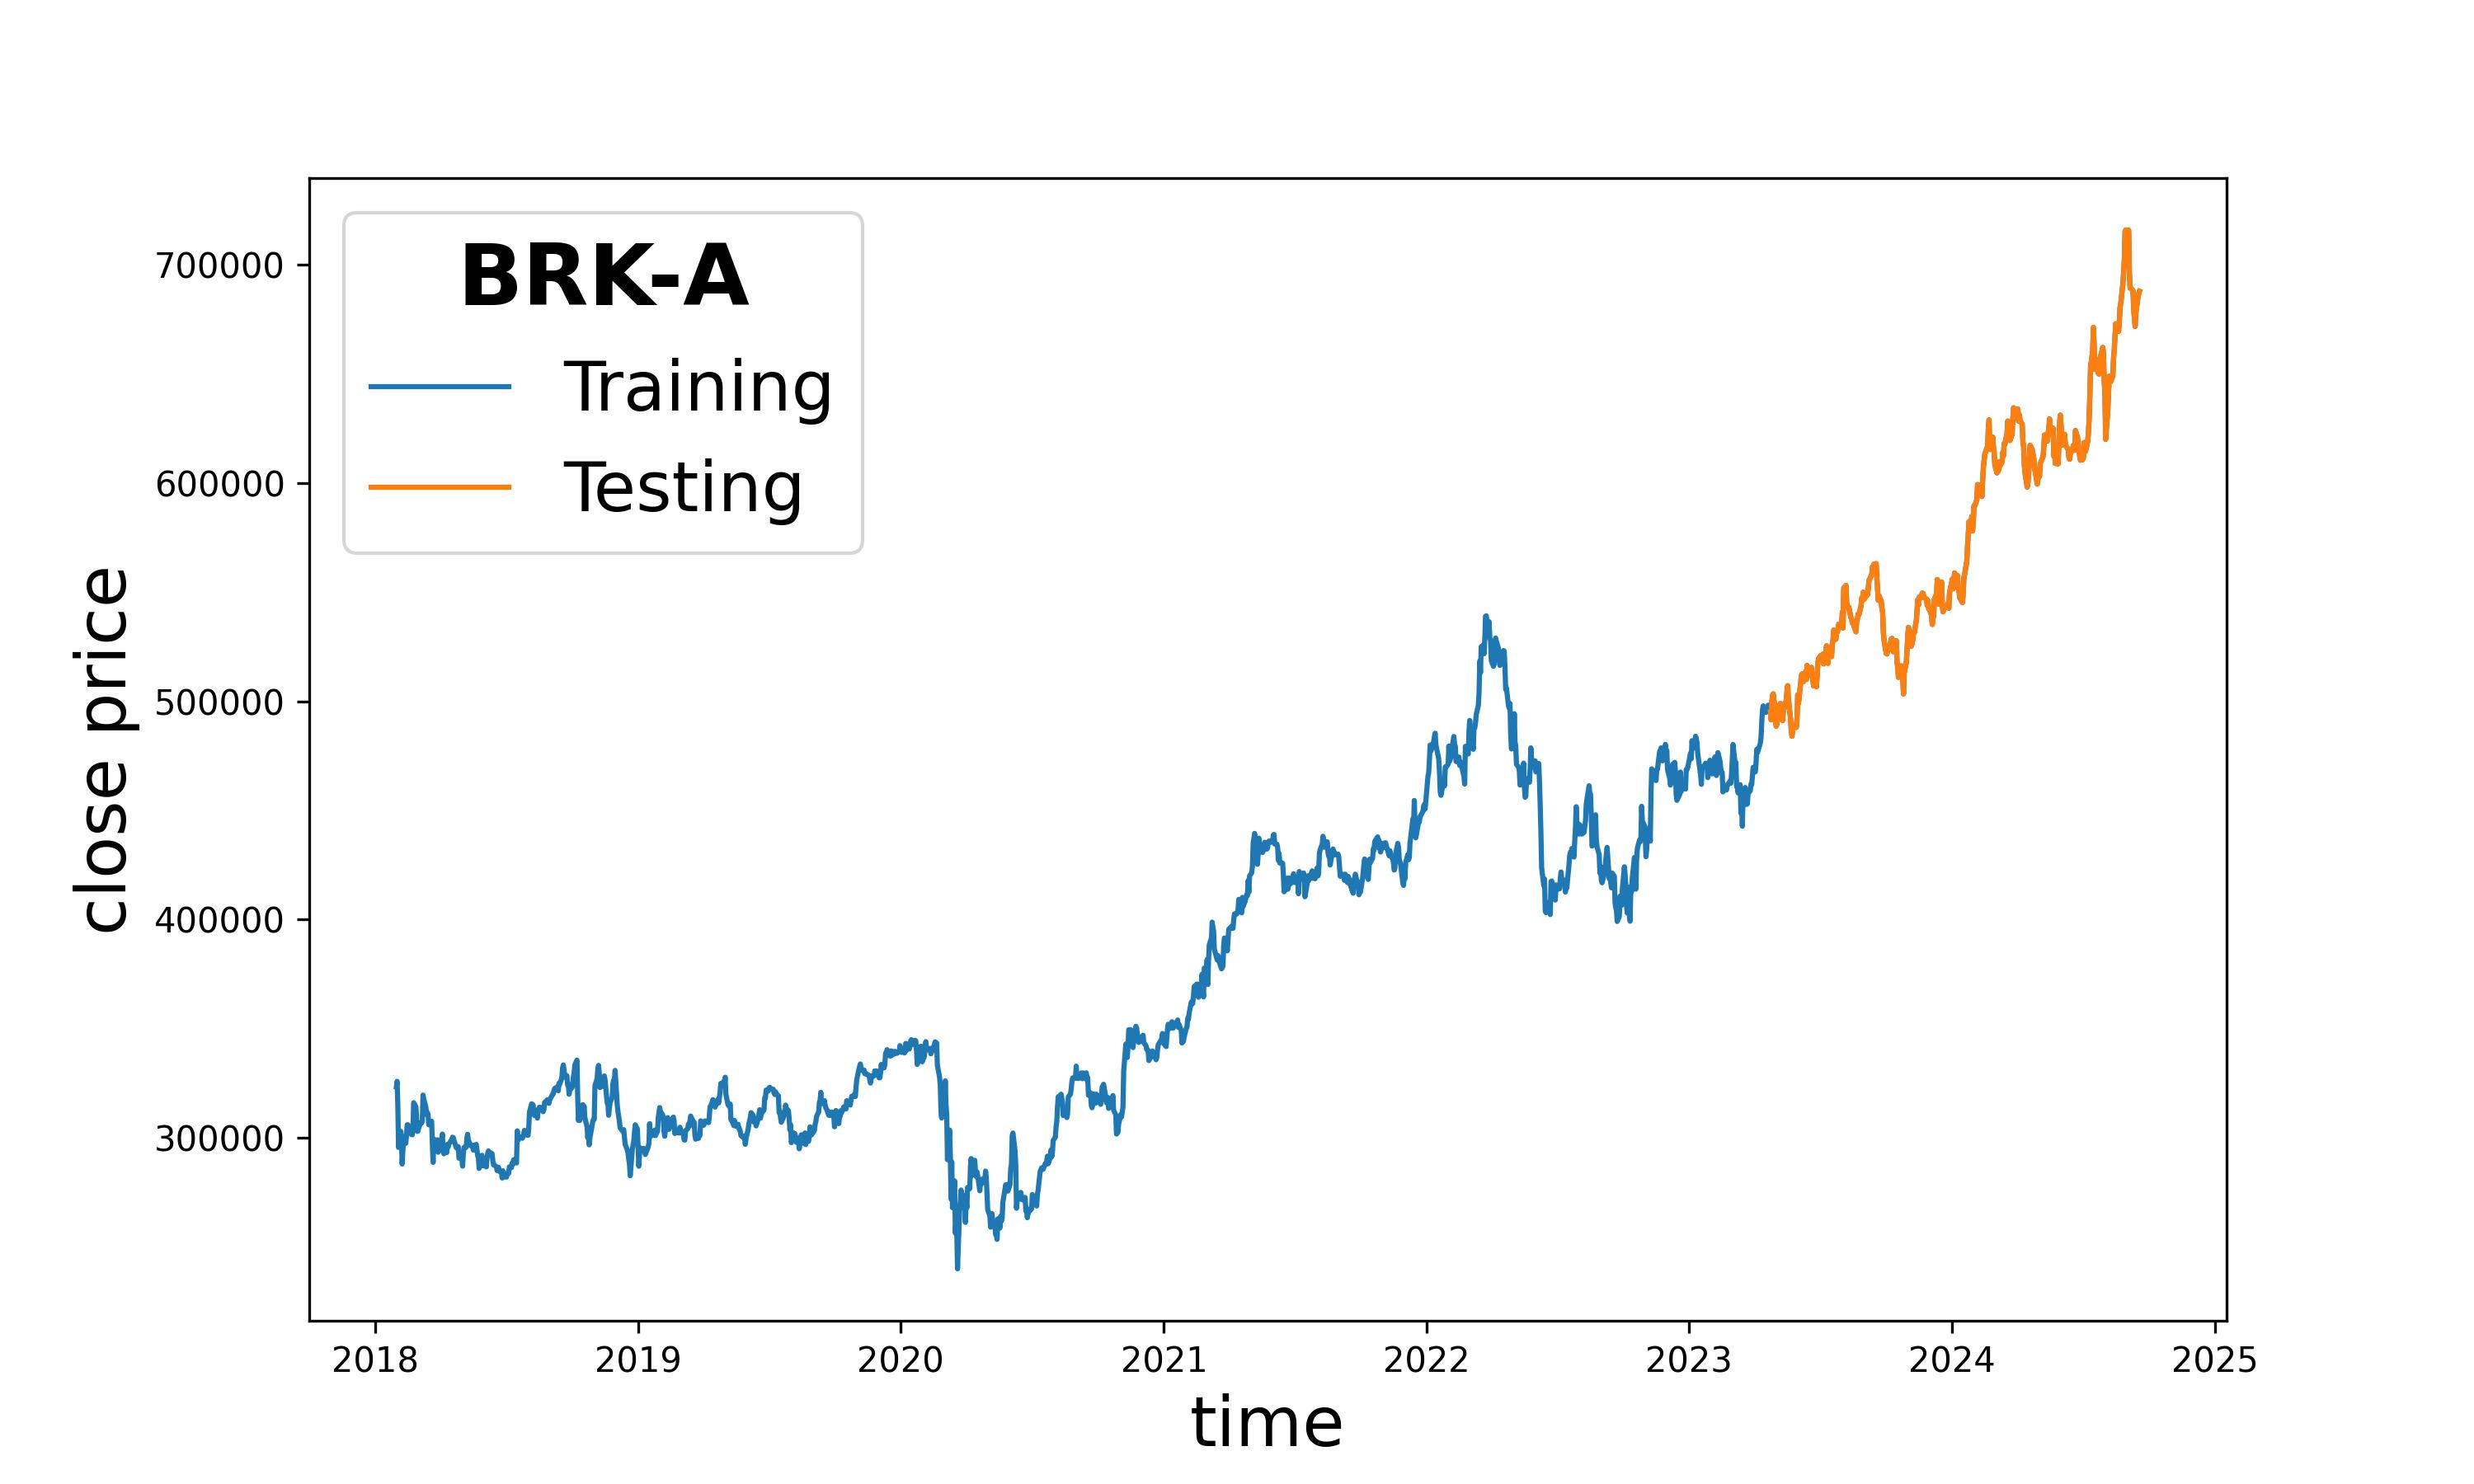
\includegraphics[width=\textwidth]{Result-Image/Result-Image3/01.BRK-A/BRK-A.jpg}
%        \caption{Training/Testing}
%        \label{fig:image1}
%    \end{subfigure}
%    
%    \begin{subfigure}[b]{0.49\textwidth}
%        \centering
%        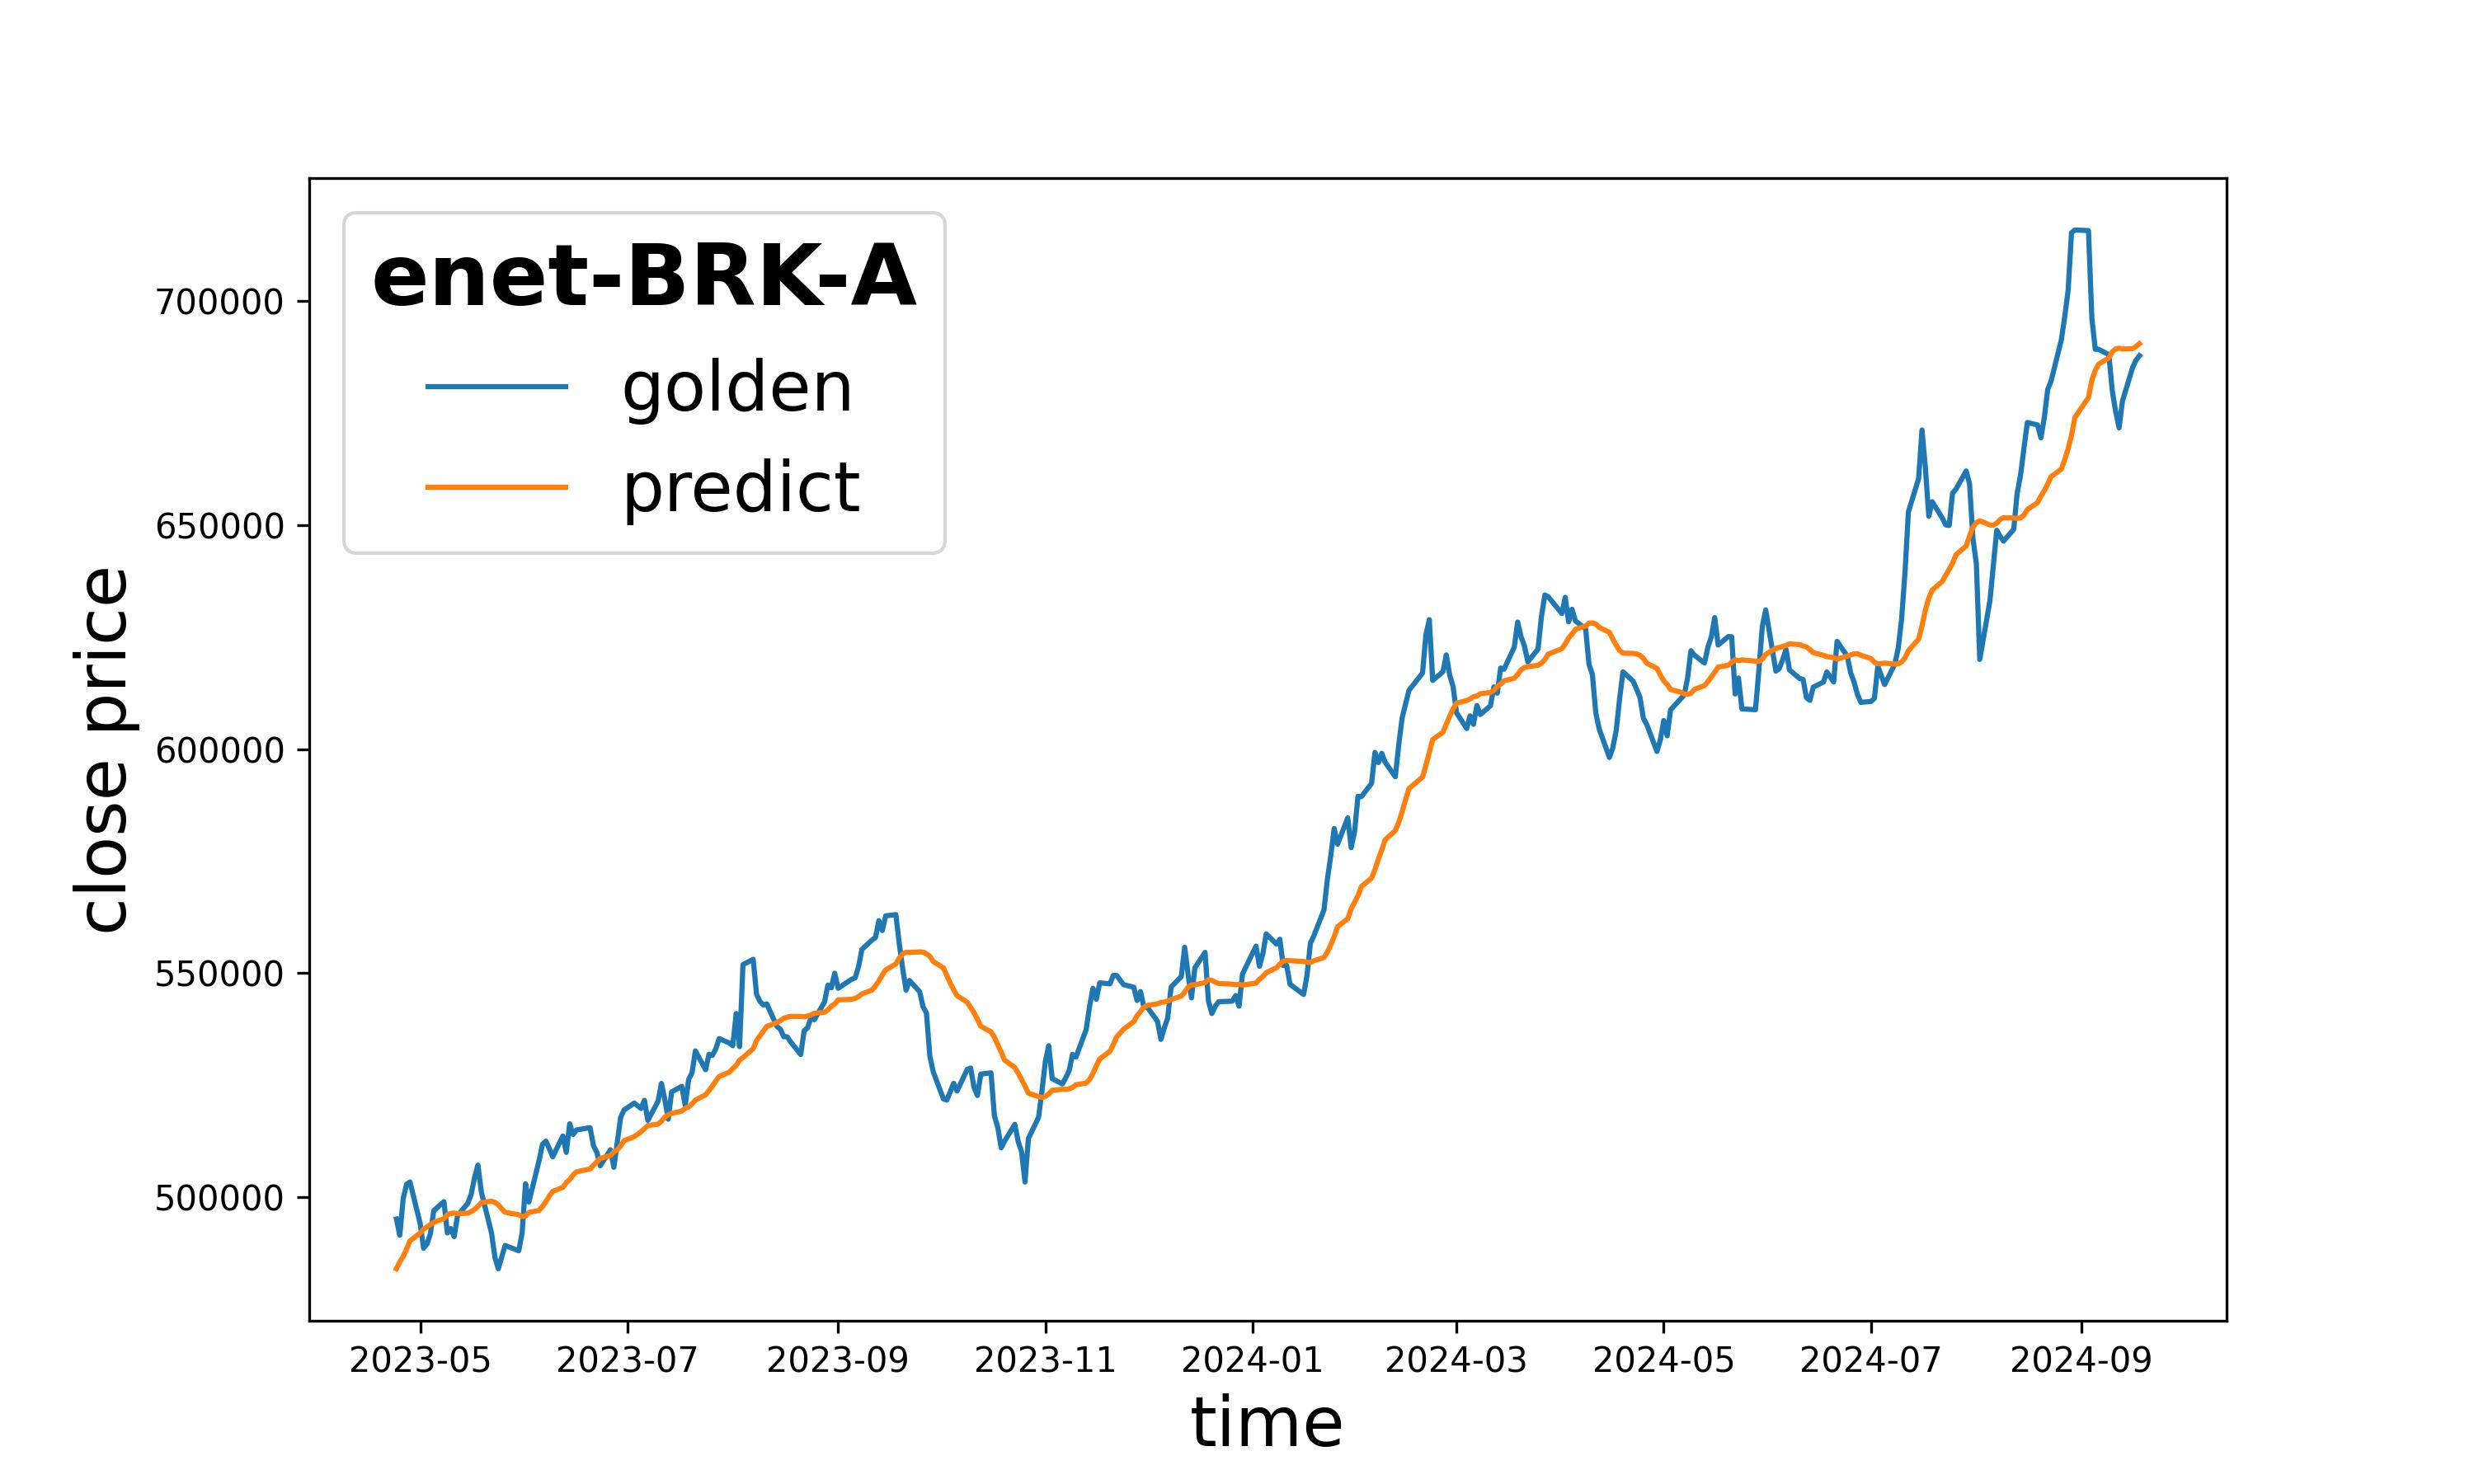
\includegraphics[width=\textwidth]{Result-Image/Result-Image3/01.BRK-A/enet-BRK-A.jpg}
%        \caption{Enet}
%        \label{fig:image1}
%    \end{subfigure}
%    \hfill
%    \begin{subfigure}[b]{0.49\textwidth}
%        \centering
%        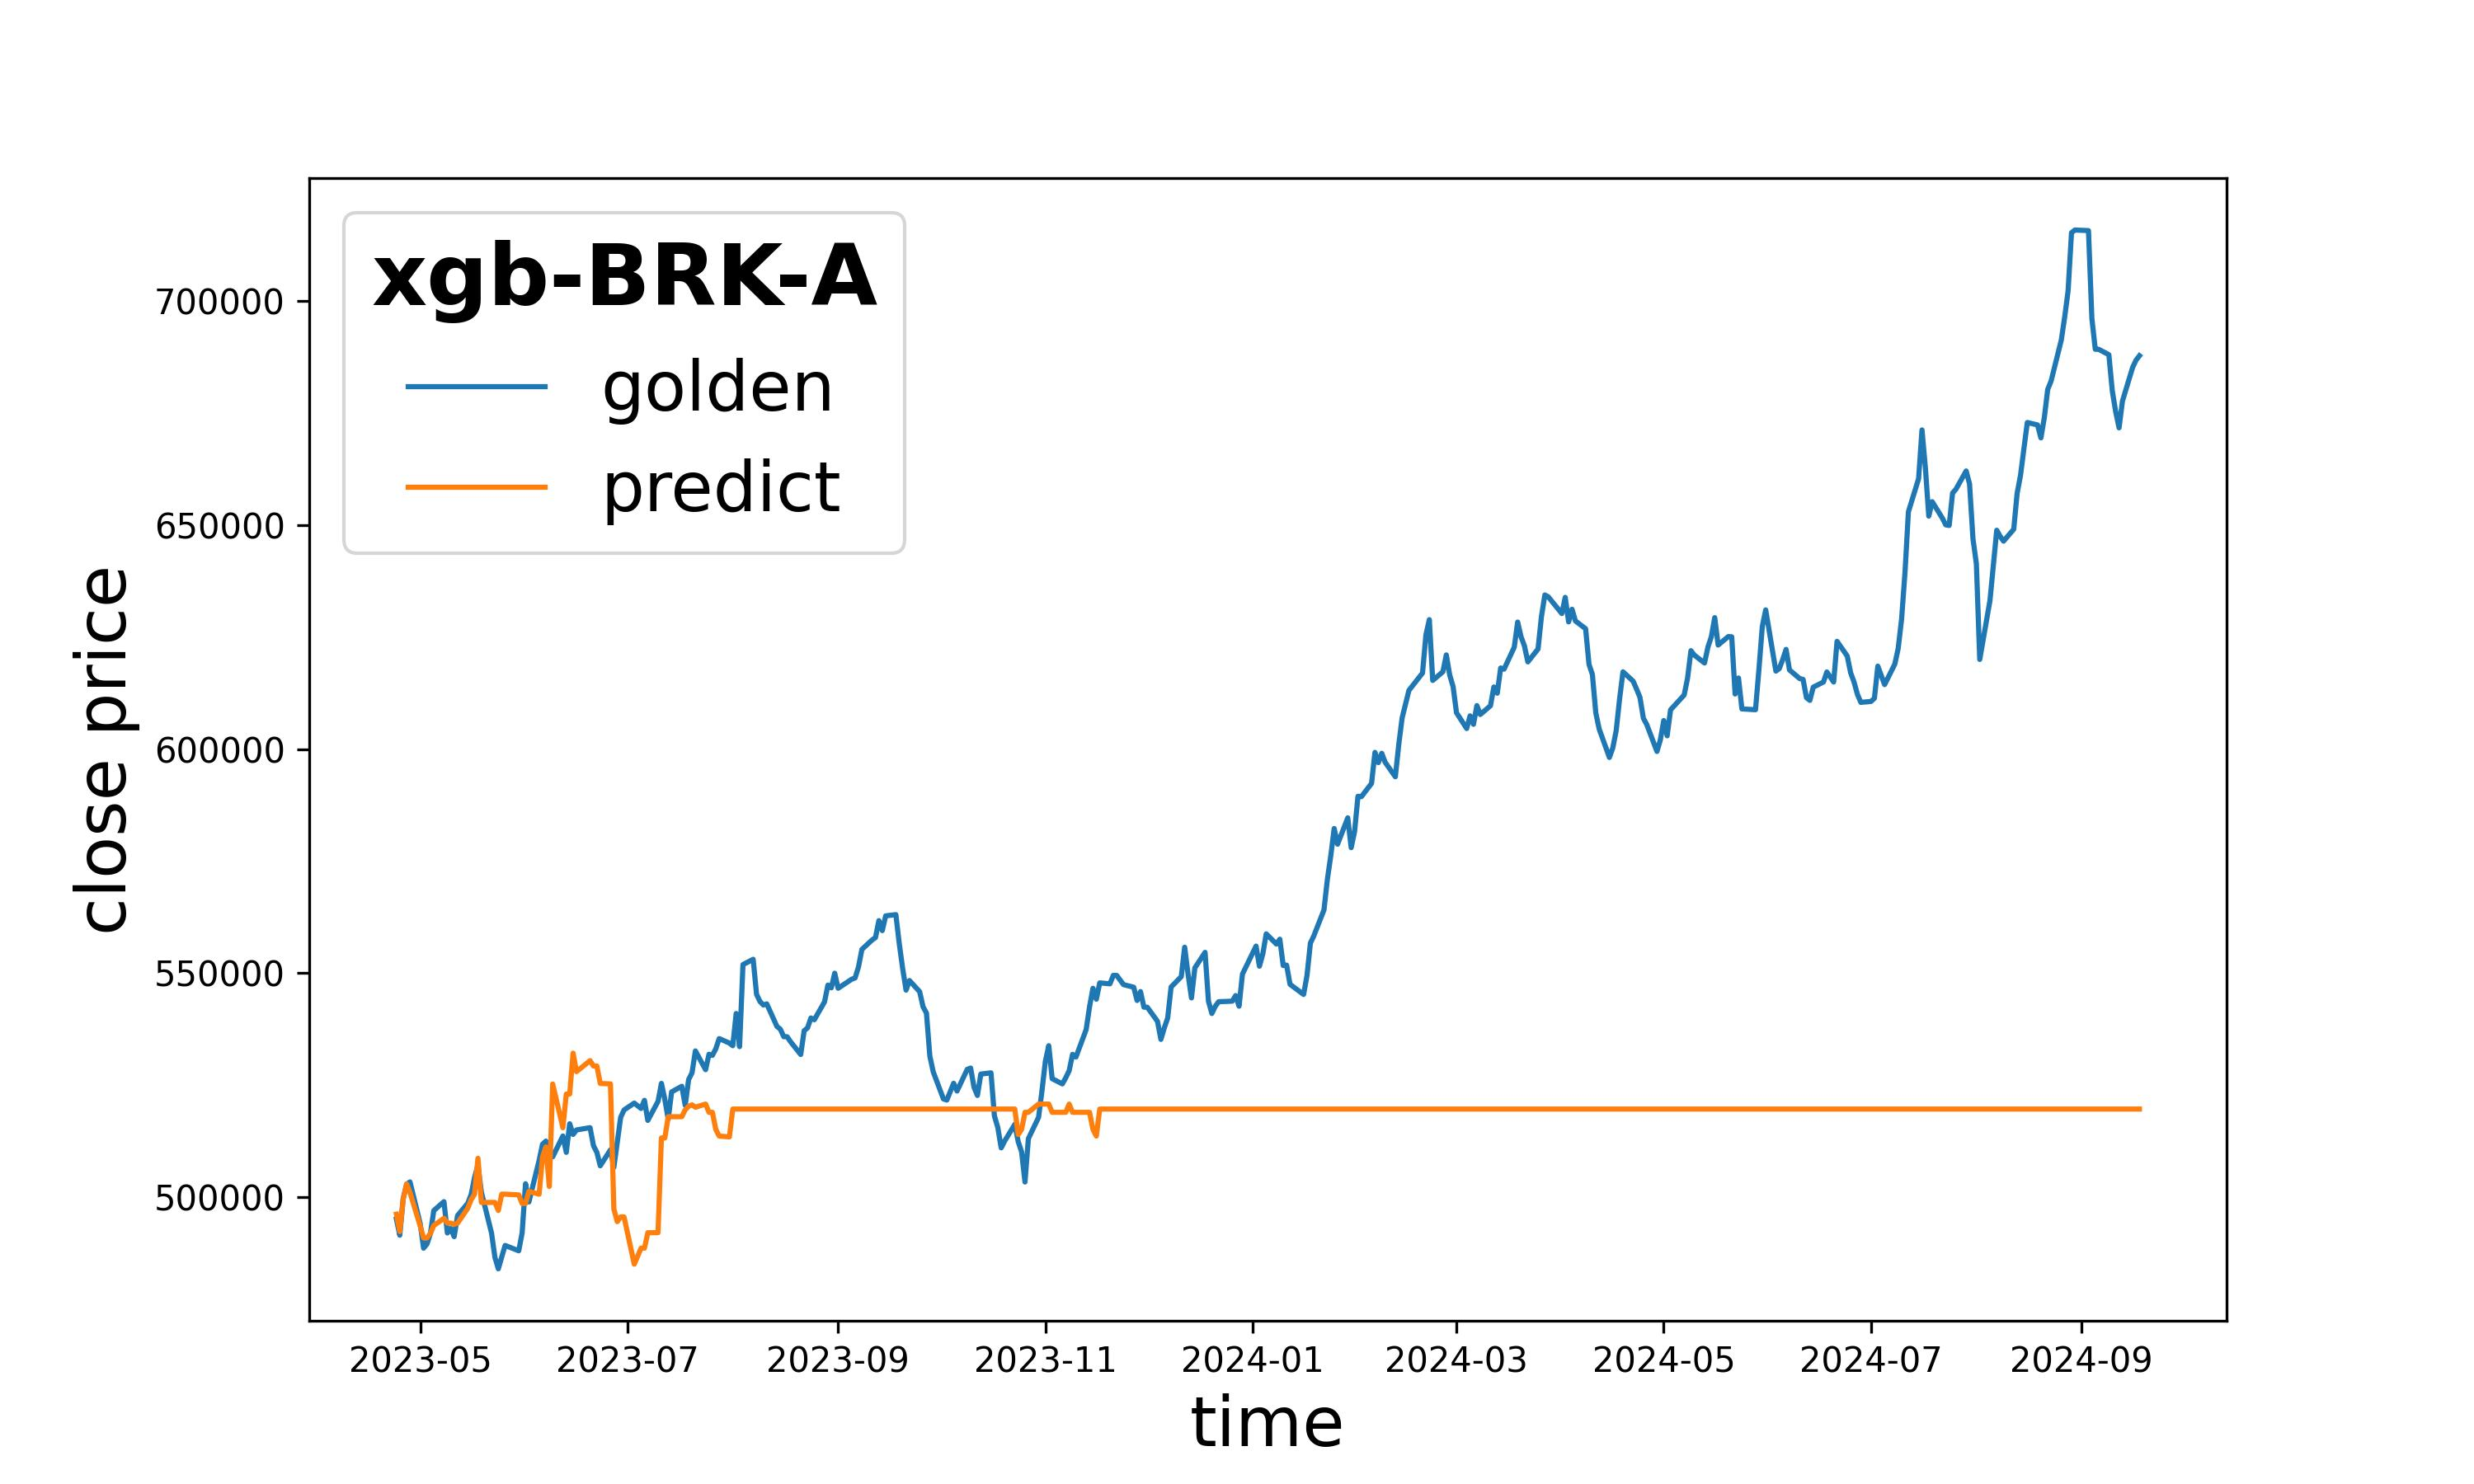
\includegraphics[width=\textwidth]{Result-Image/Result-Image3/01.BRK-A/xgb-BRK-A.jpg}
%        \caption{XGBoost}
%        \label{fig:image2}
%    \end{subfigure}
%    
%    % 두 번째 행
%    \vskip\baselineskip
%    \begin{subfigure}[b]{0.49\textwidth}
%        \centering
%        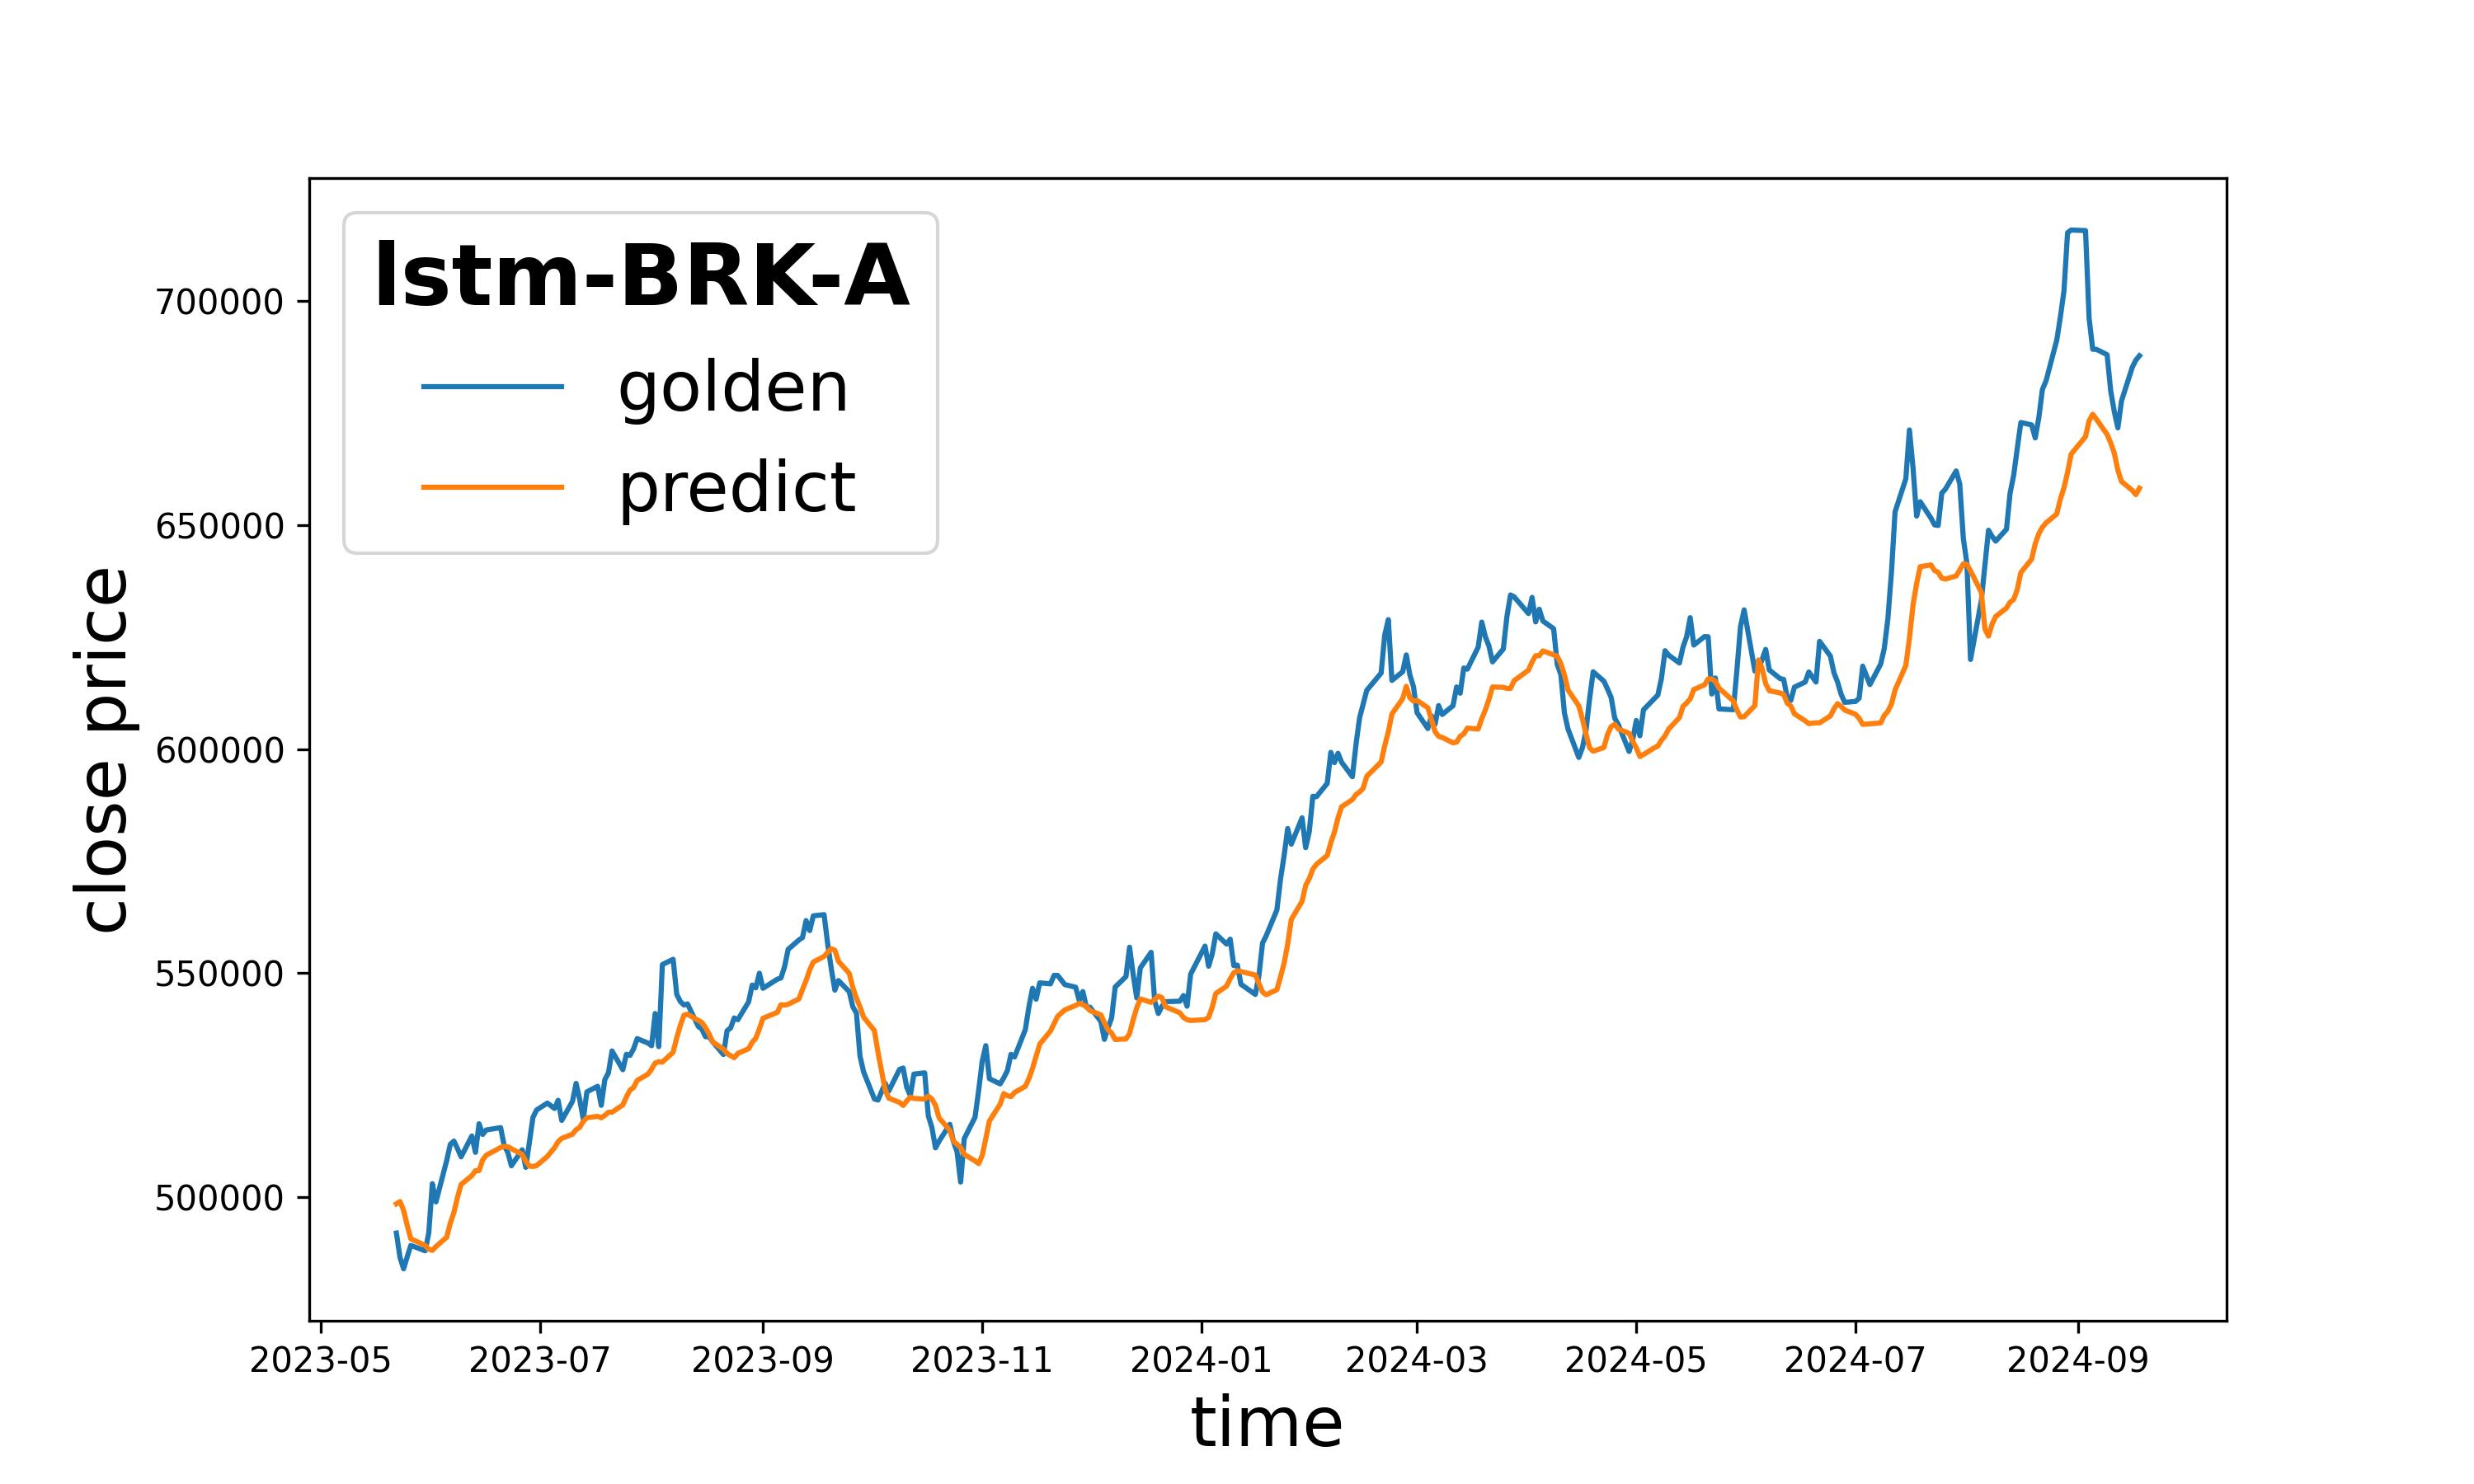
\includegraphics[width=\textwidth]{Result-Image/Result-Image3/01.BRK-A/lstm-BRK-A.jpg}
%        \caption{LSTM}
%        \label{fig:image3}
%    \end{subfigure}
%    \hfill
%    \begin{subfigure}[b]{0.49\textwidth}
%        \centering
%        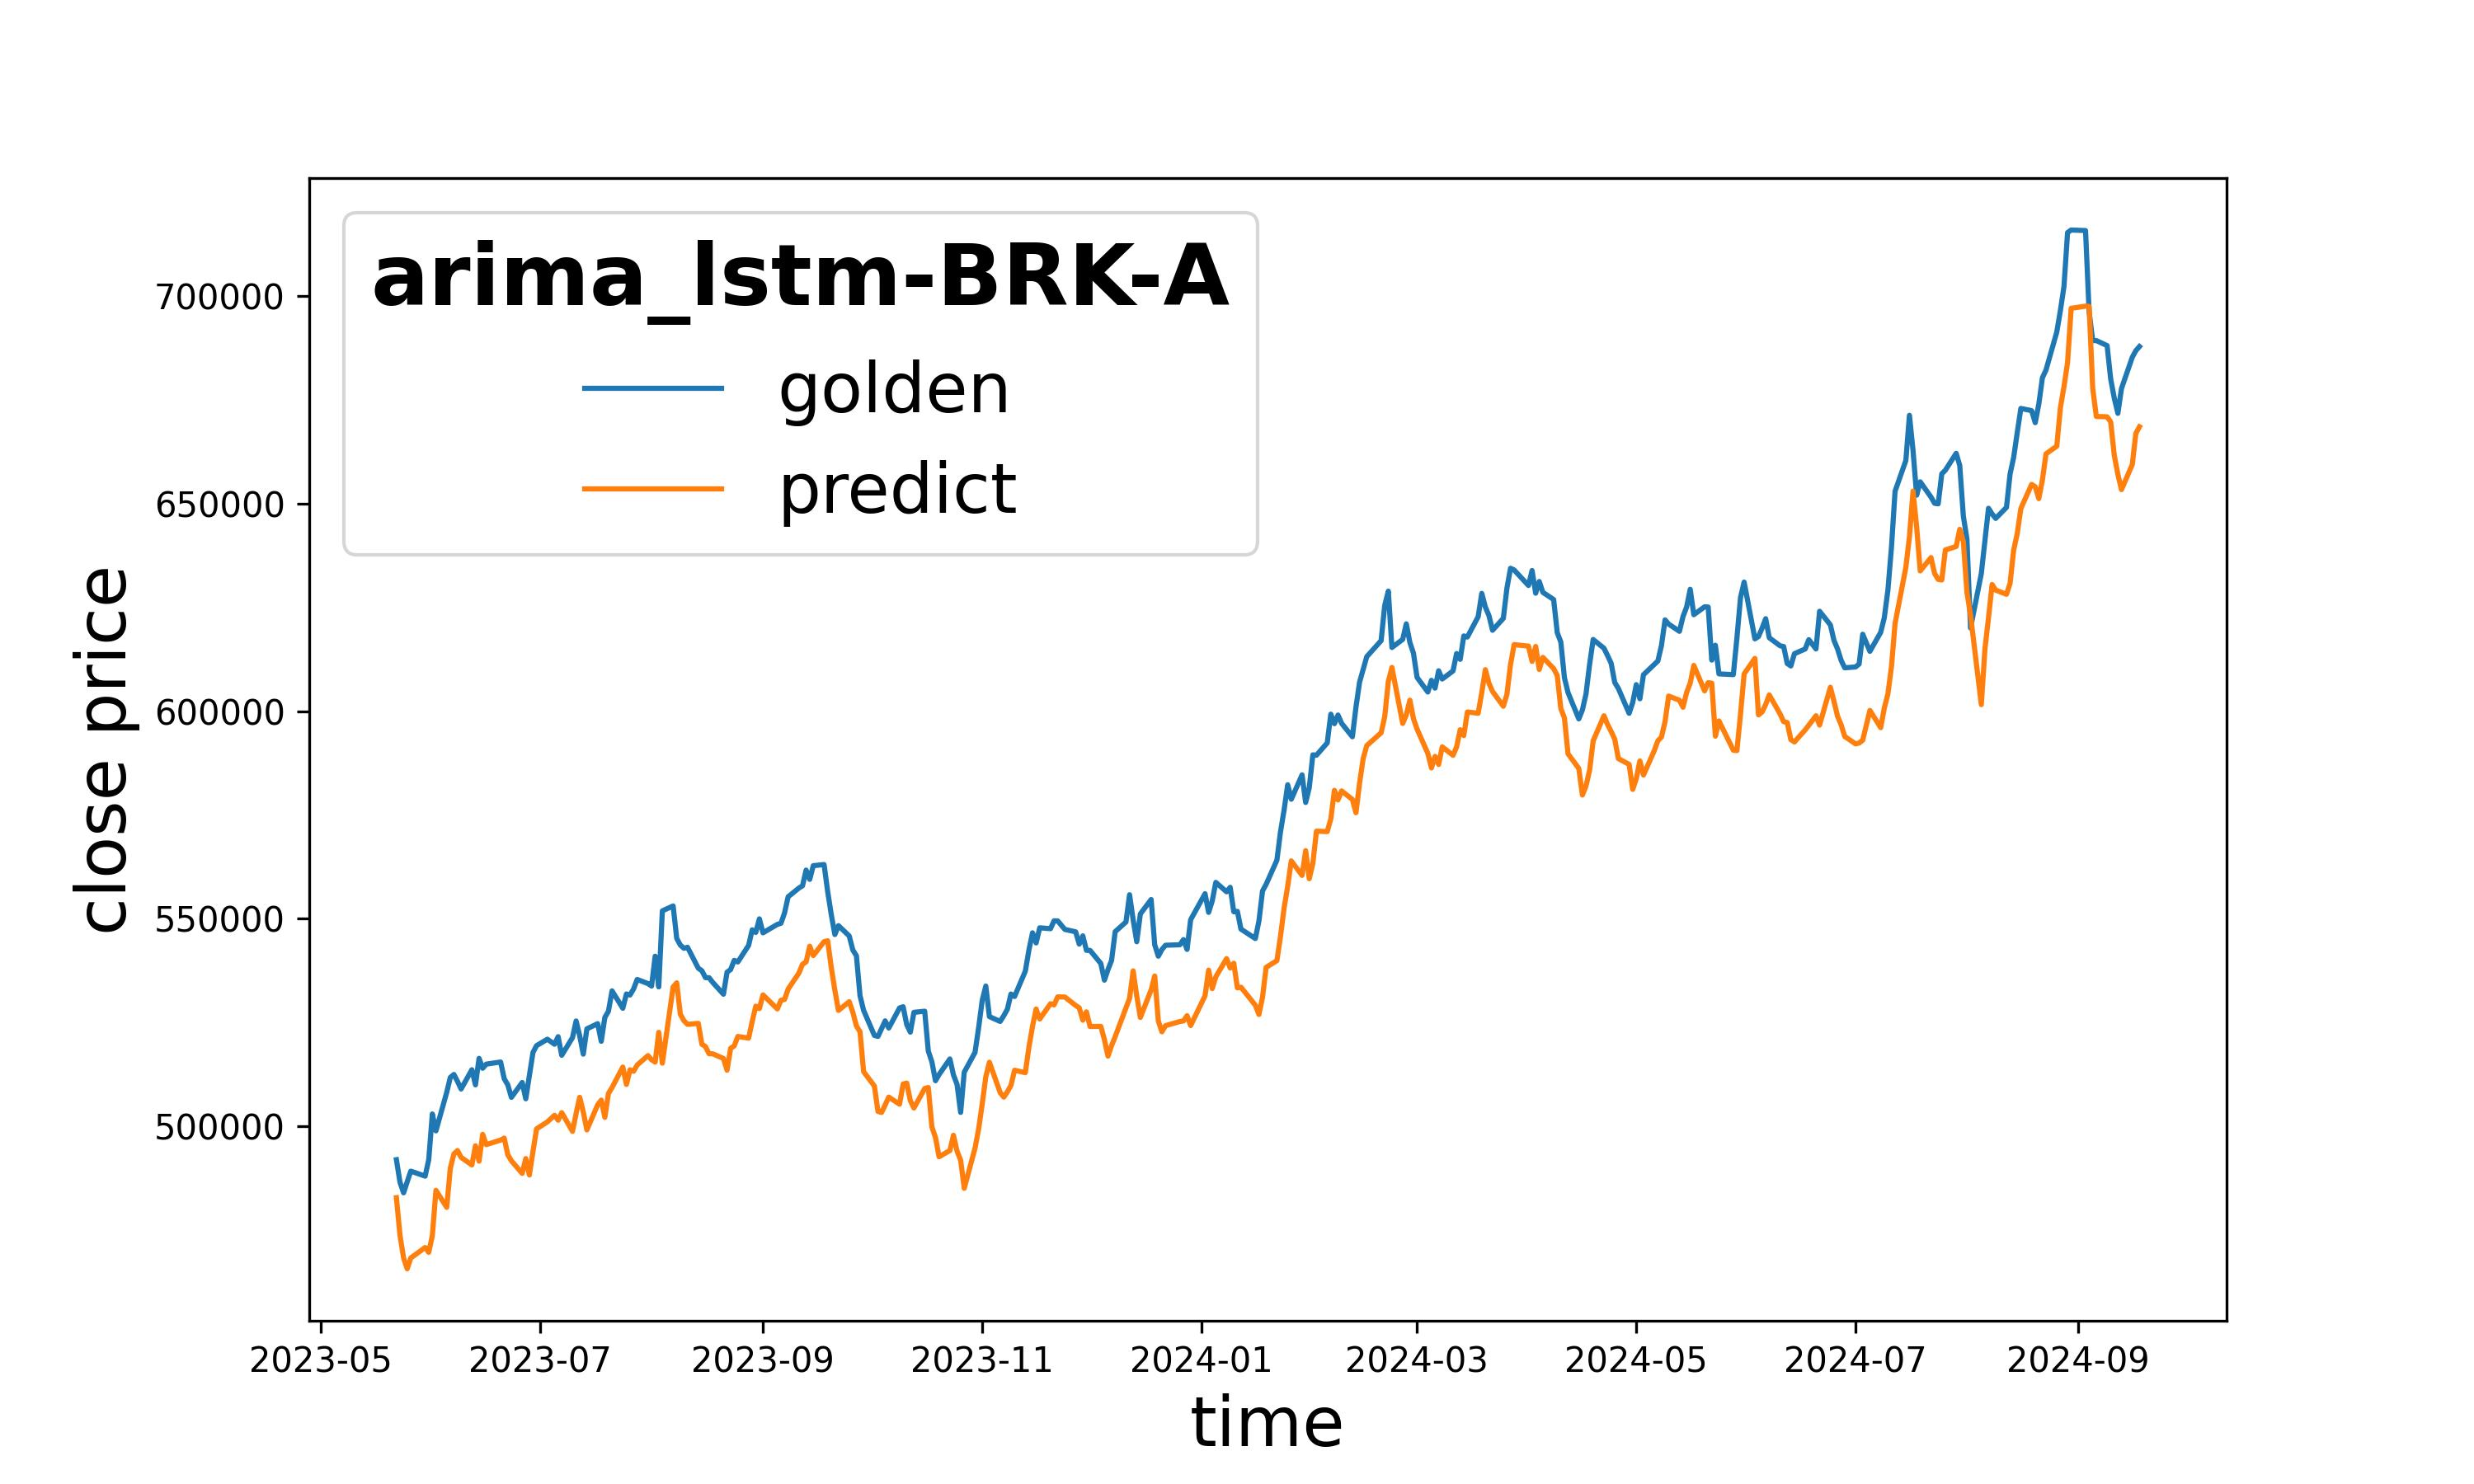
\includegraphics[width=\textwidth]{Result-Image/Result-Image3/01.BRK-A/arima_lstm-BRK-A.jpg}
%        \caption{ARIMA-LSTM}
%        \label{fig:image4}
%    \end{subfigure}
%    
%    \caption{BRK-A}
%    \label{fig:2x2grid}
%\end{figure}
%
%%\subsection{DPZ}
%\begin{figure}[ht]
%    \centering
%
%    \begin{subfigure}[b]{0.49\textwidth}
%        \centering
%        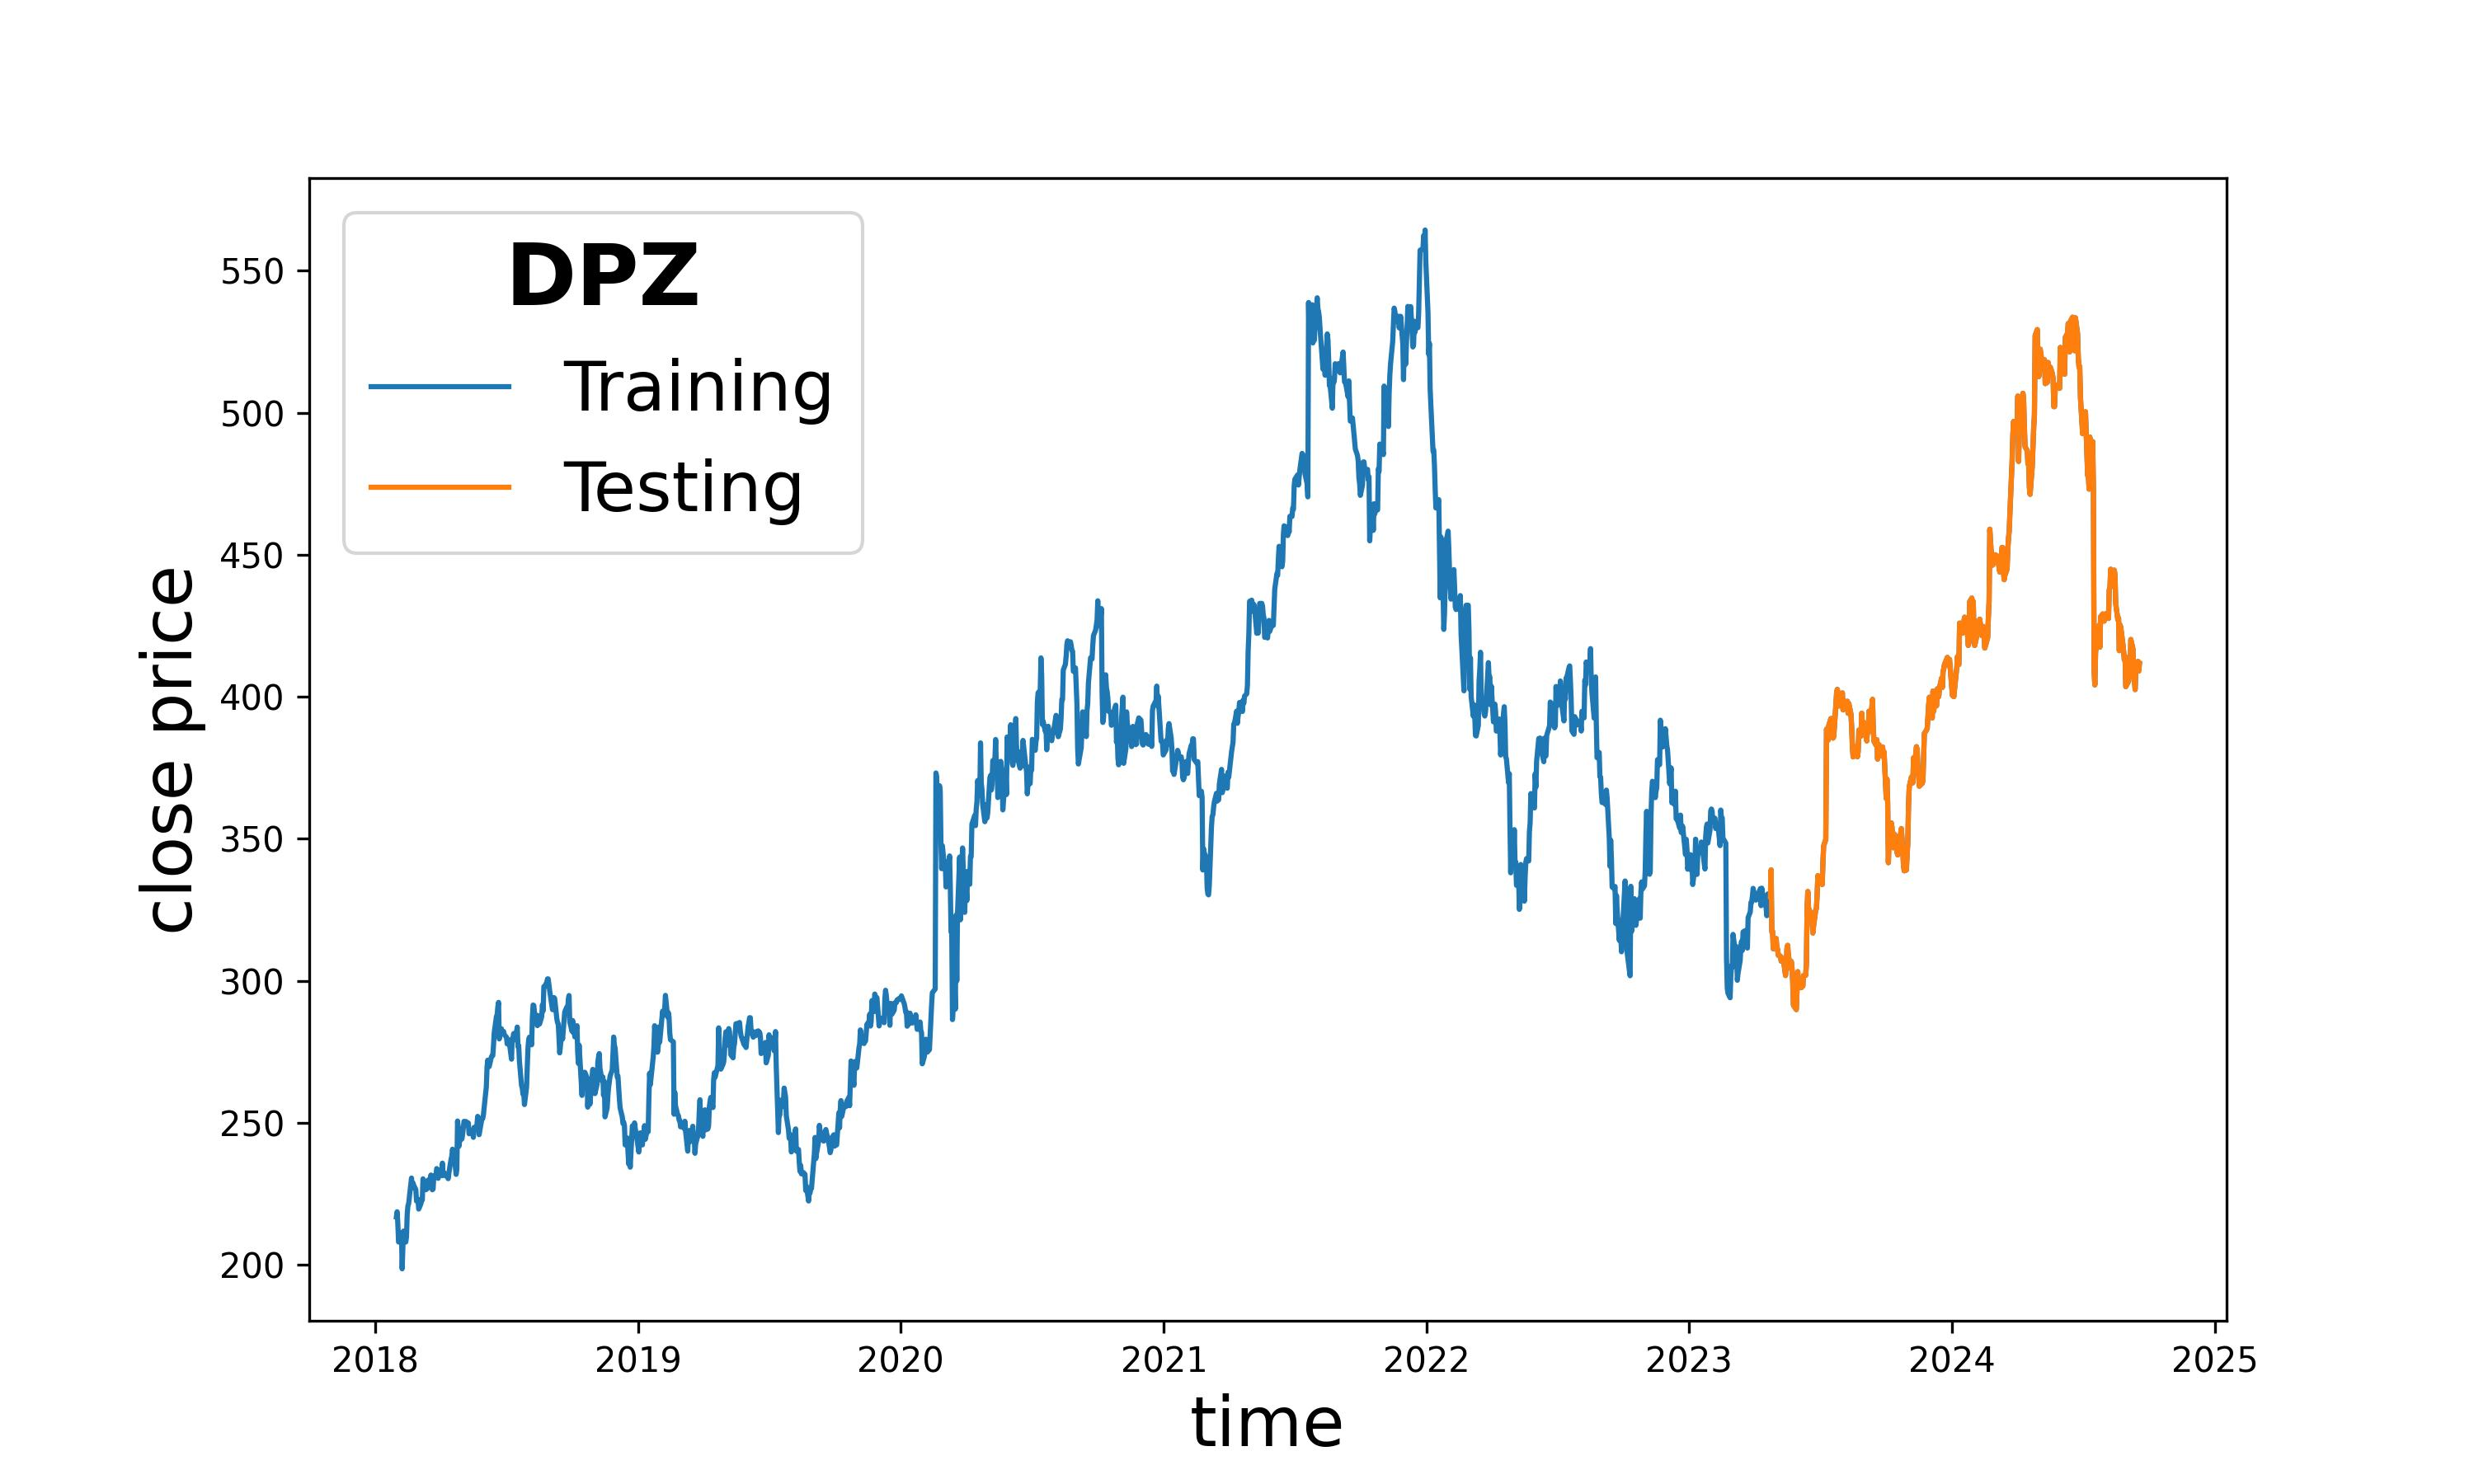
\includegraphics[width=\textwidth]{Result-Image/Result-Image3/02.DPZ/DPZ.jpg}
%        \caption{Training/Testing}
%        \label{fig:image1}
%    \end{subfigure}
%
%    % first row 첫 번째 행
%    \begin{subfigure}[b]{0.49\textwidth}
%        \centering
%        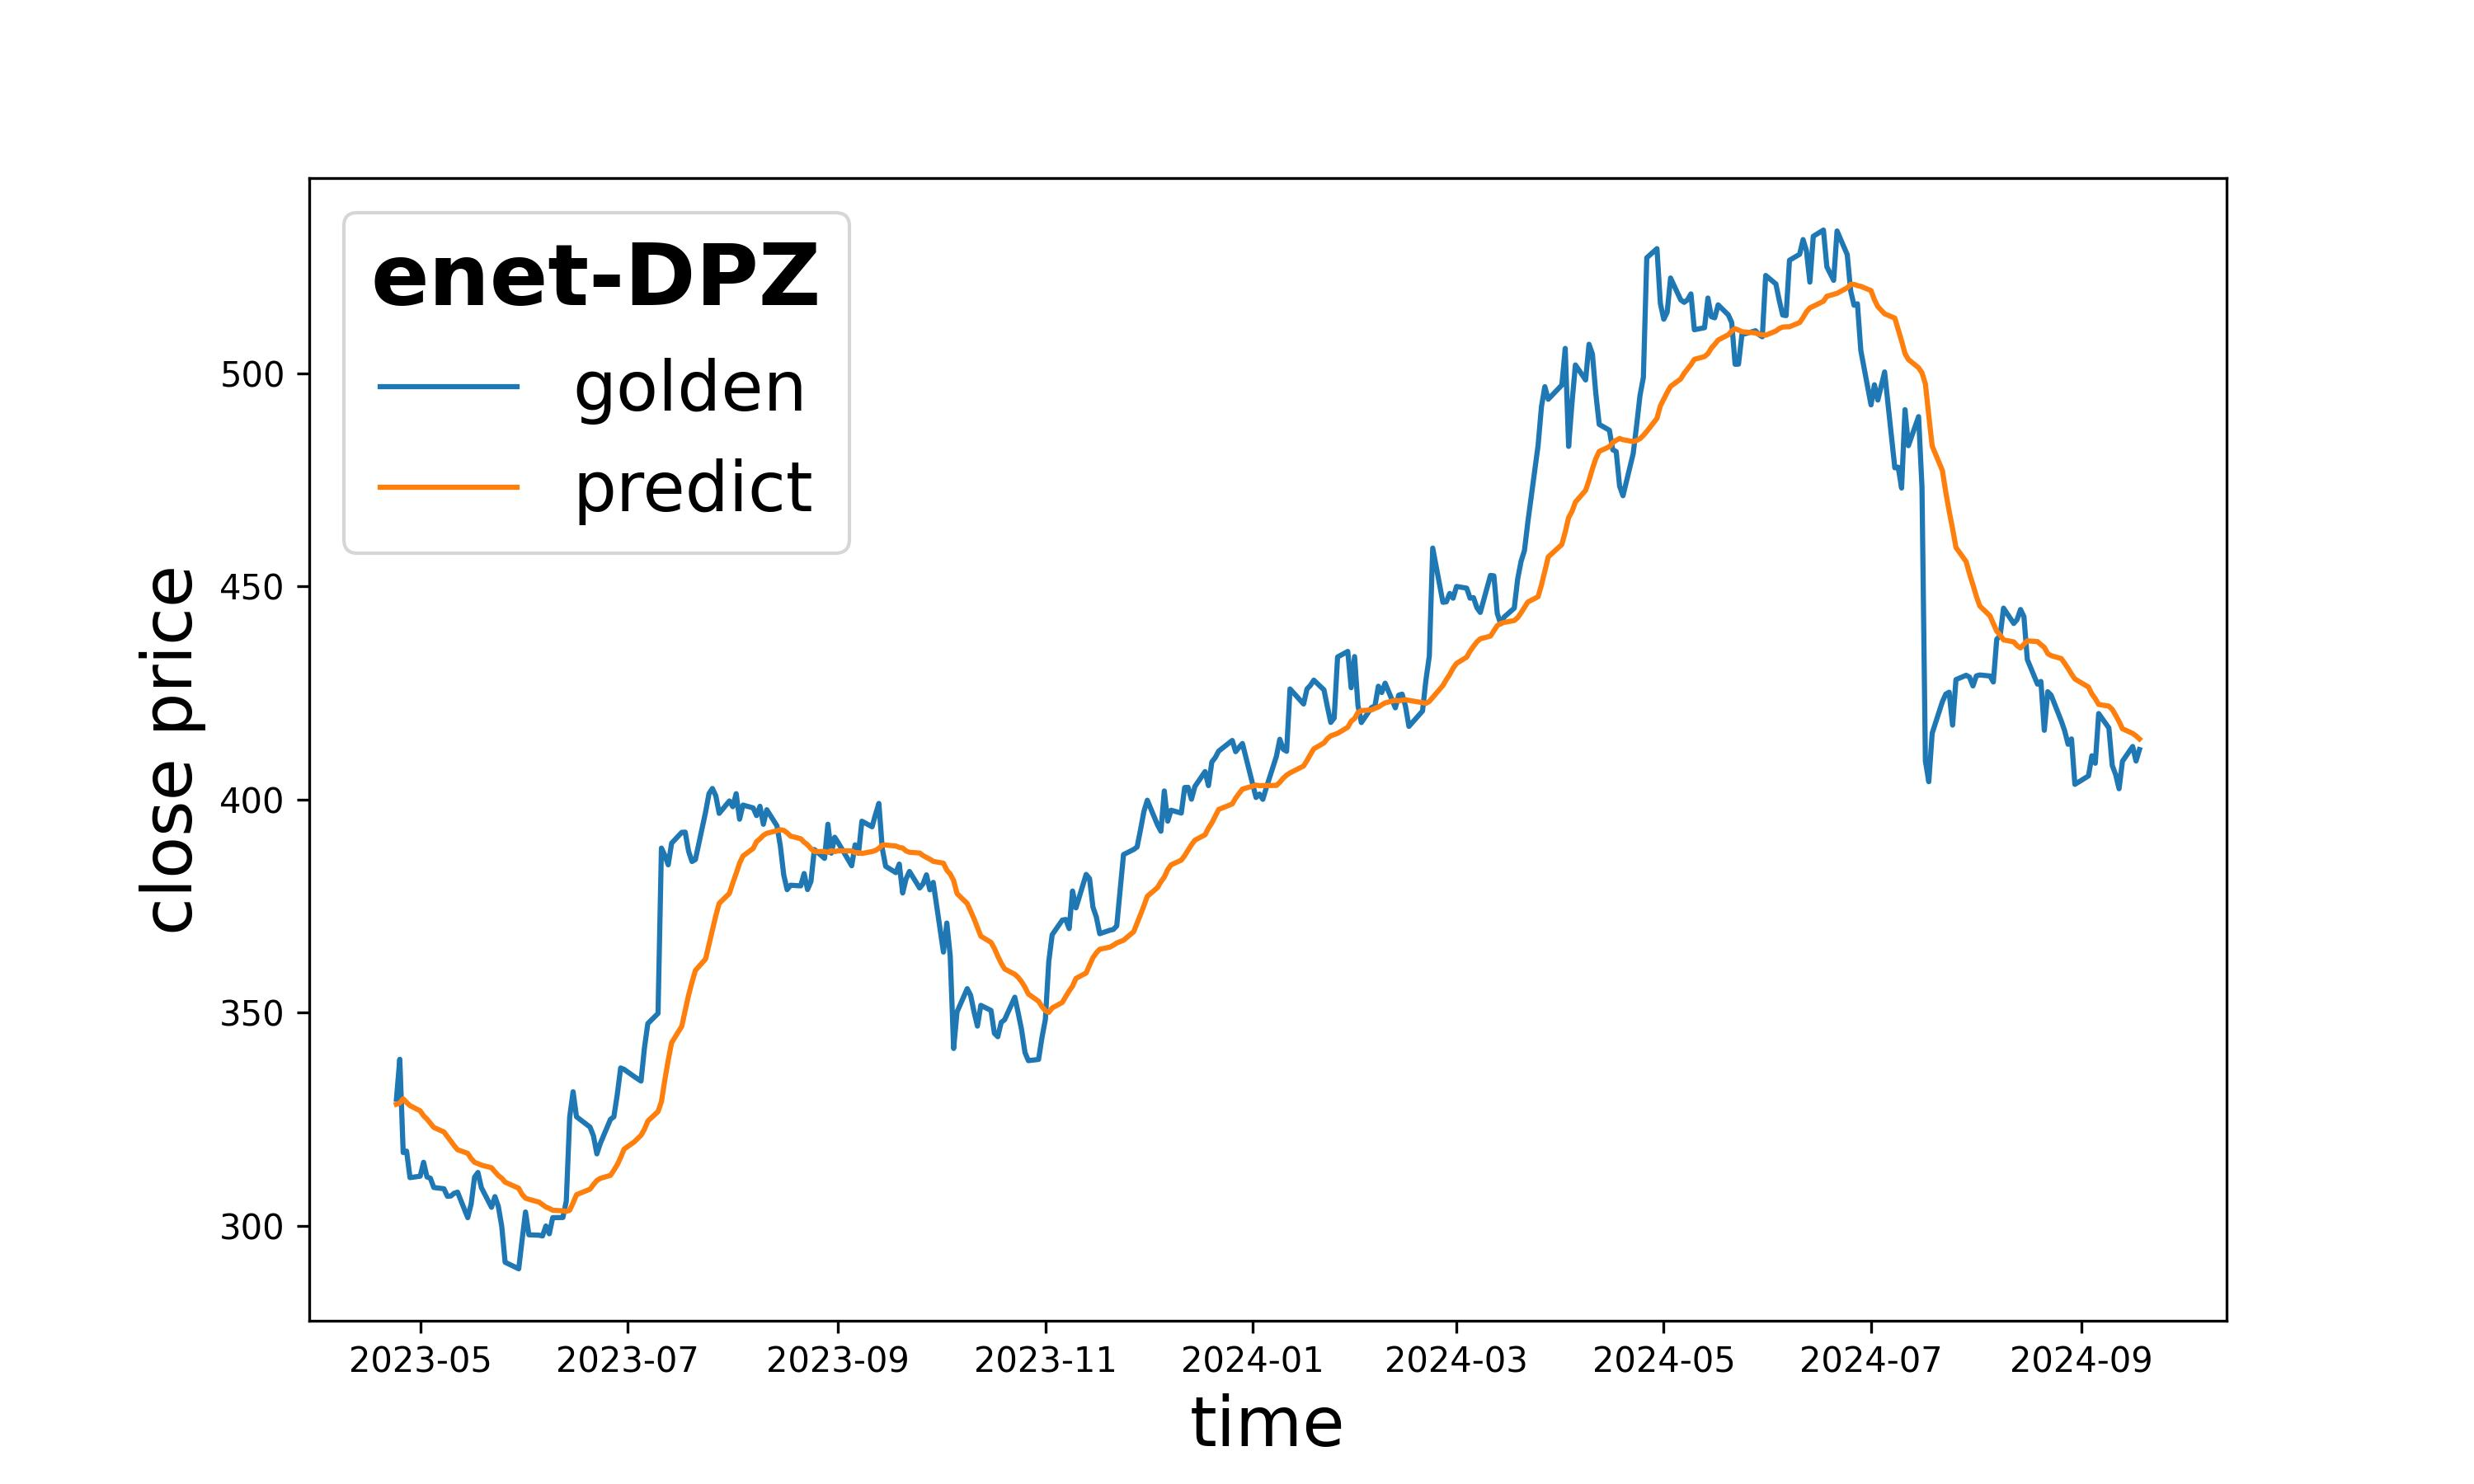
\includegraphics[width=\textwidth]{Result-Image/Result-Image3/02.DPZ/enet-DPZ.jpg}
%        \caption{Enet}
%        \label{fig:image1}
%    \end{subfigure}
%    \hfill
%    \begin{subfigure}[b]{0.49\textwidth}
%        \centering
%        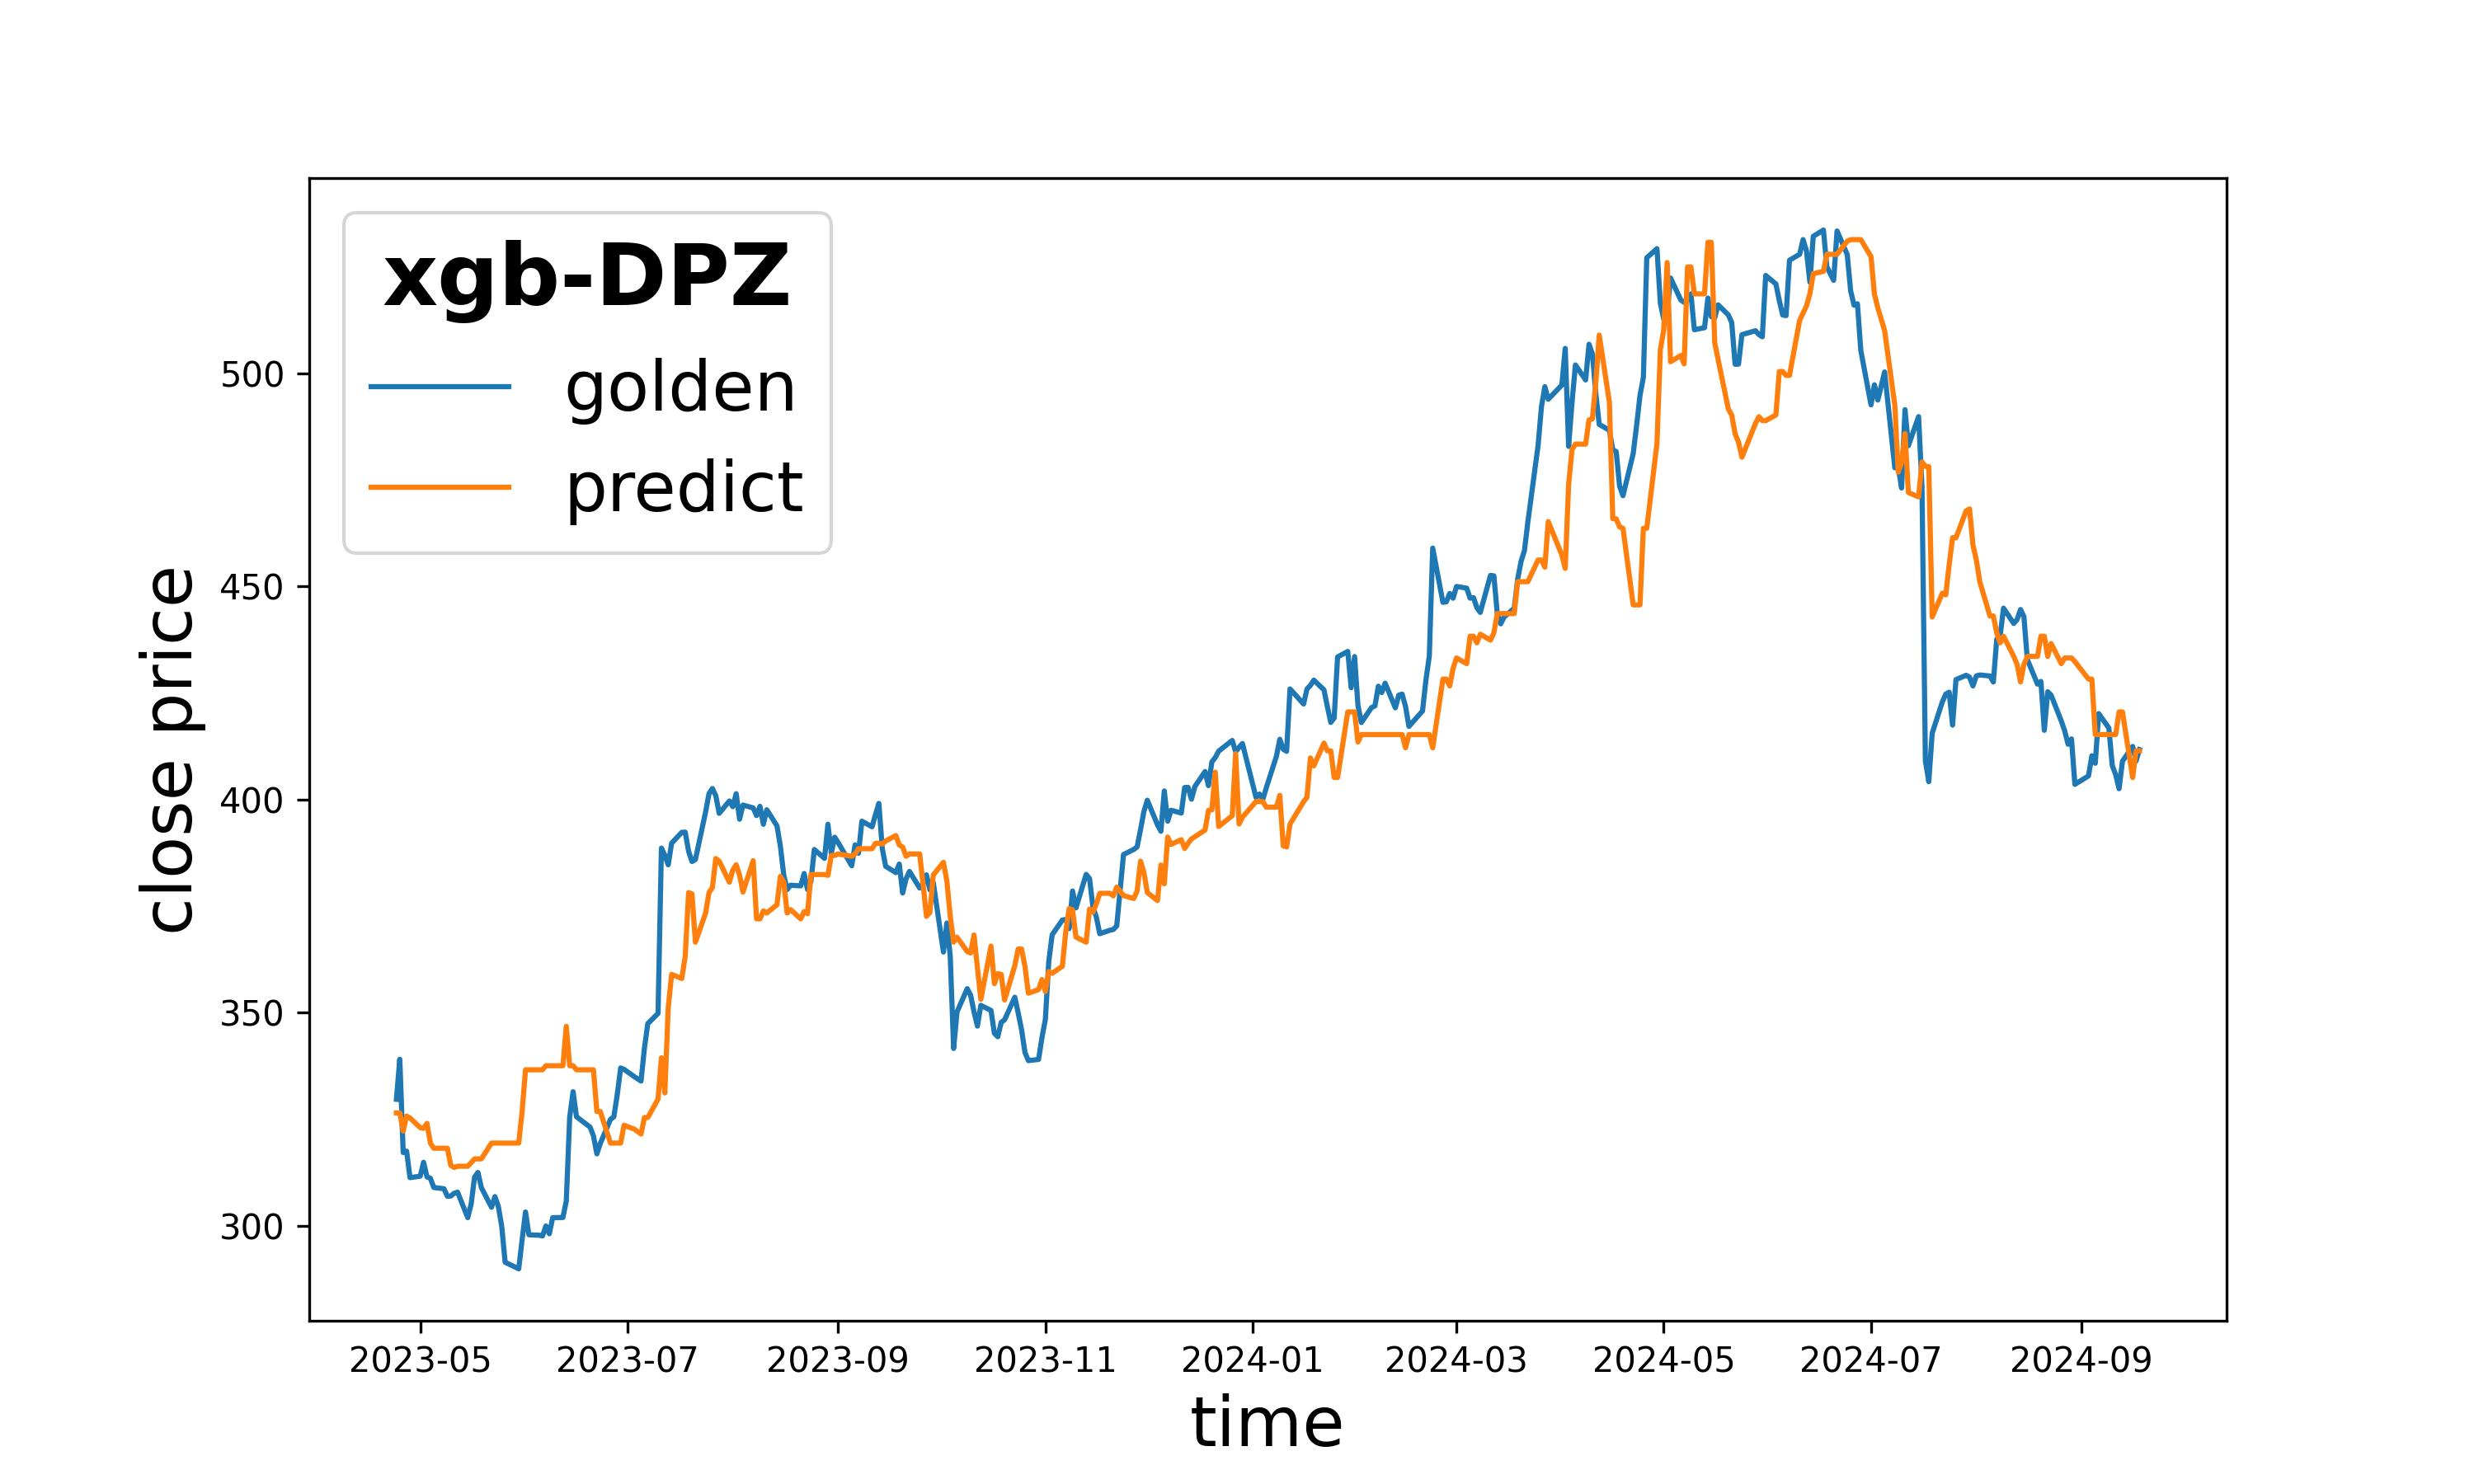
\includegraphics[width=\textwidth]{Result-Image/Result-Image3/02.DPZ/xgb-DPZ.jpg}
%        \caption{XGBoost}
%        \label{fig:image2}
%    \end{subfigure}
%    
%    % 두 번째 행
%    \vskip\baselineskip
%    \begin{subfigure}[b]{0.49\textwidth}
%        \centering
%        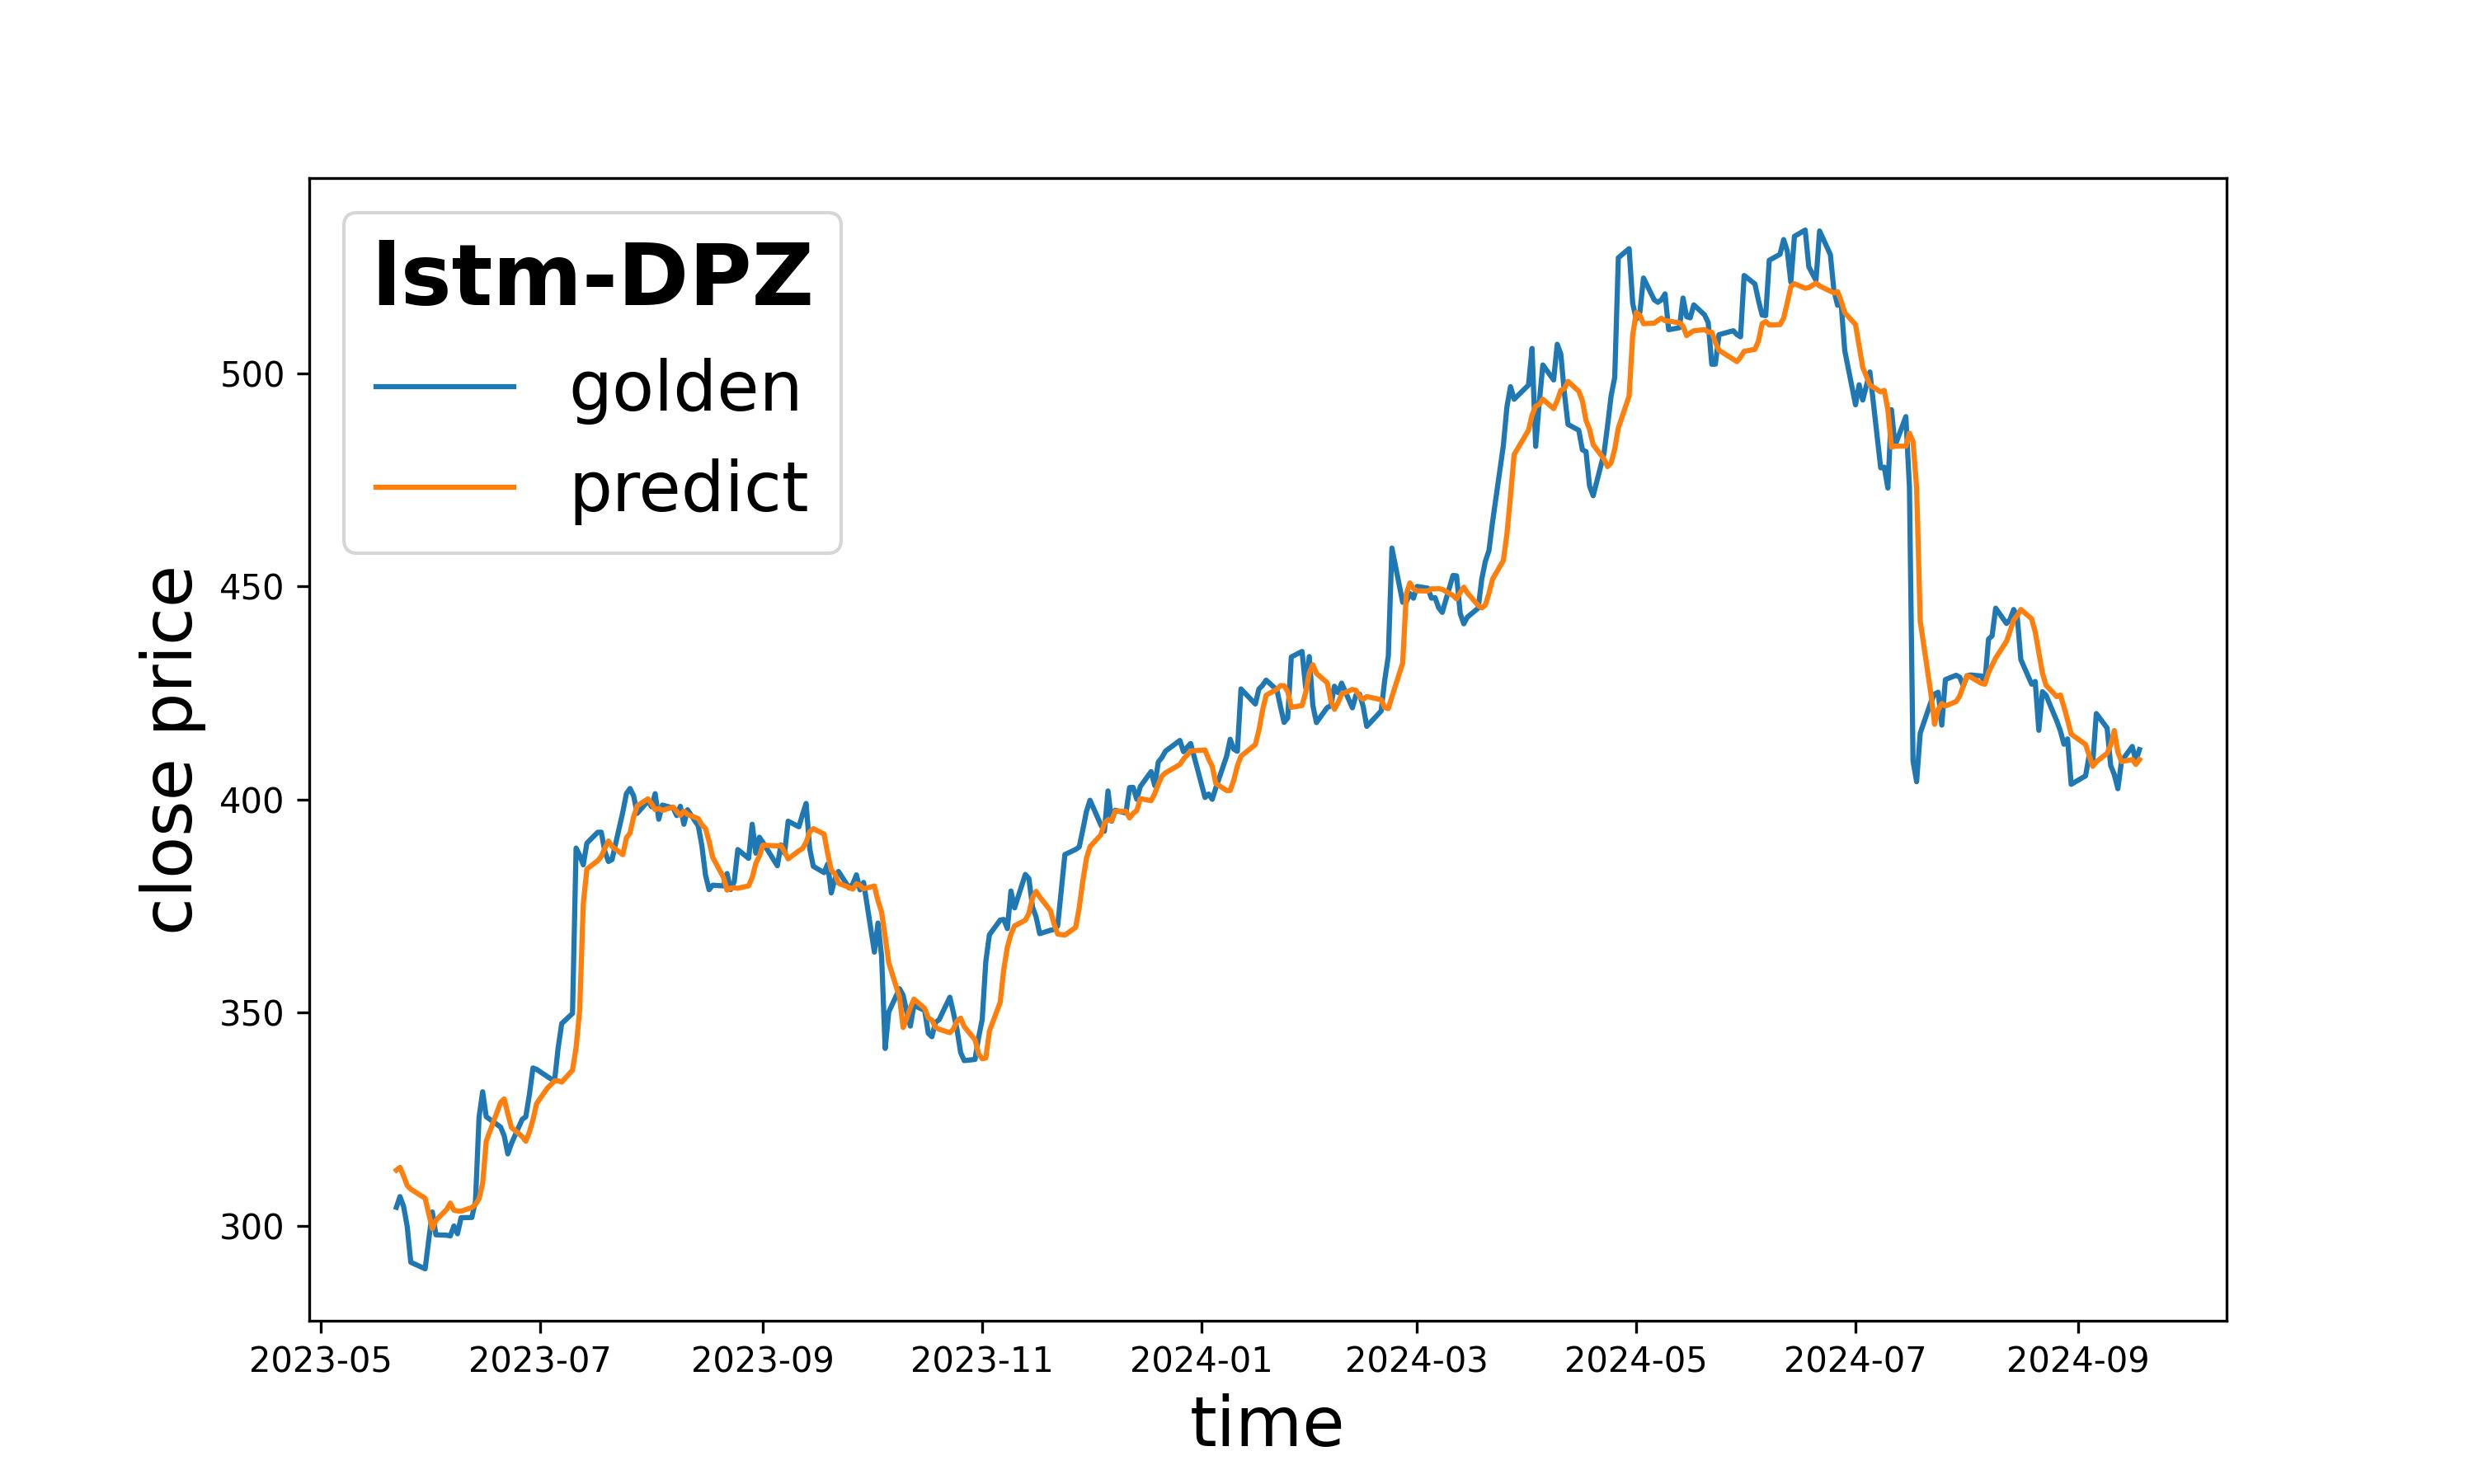
\includegraphics[width=\textwidth]{Result-Image/Result-Image3/02.DPZ/lstm-DPZ.jpg}
%        \caption{LSTM}
%        \label{fig:image3}
%    \end{subfigure}
%    \hfill
%    \begin{subfigure}[b]{0.49\textwidth}
%        \centering
%        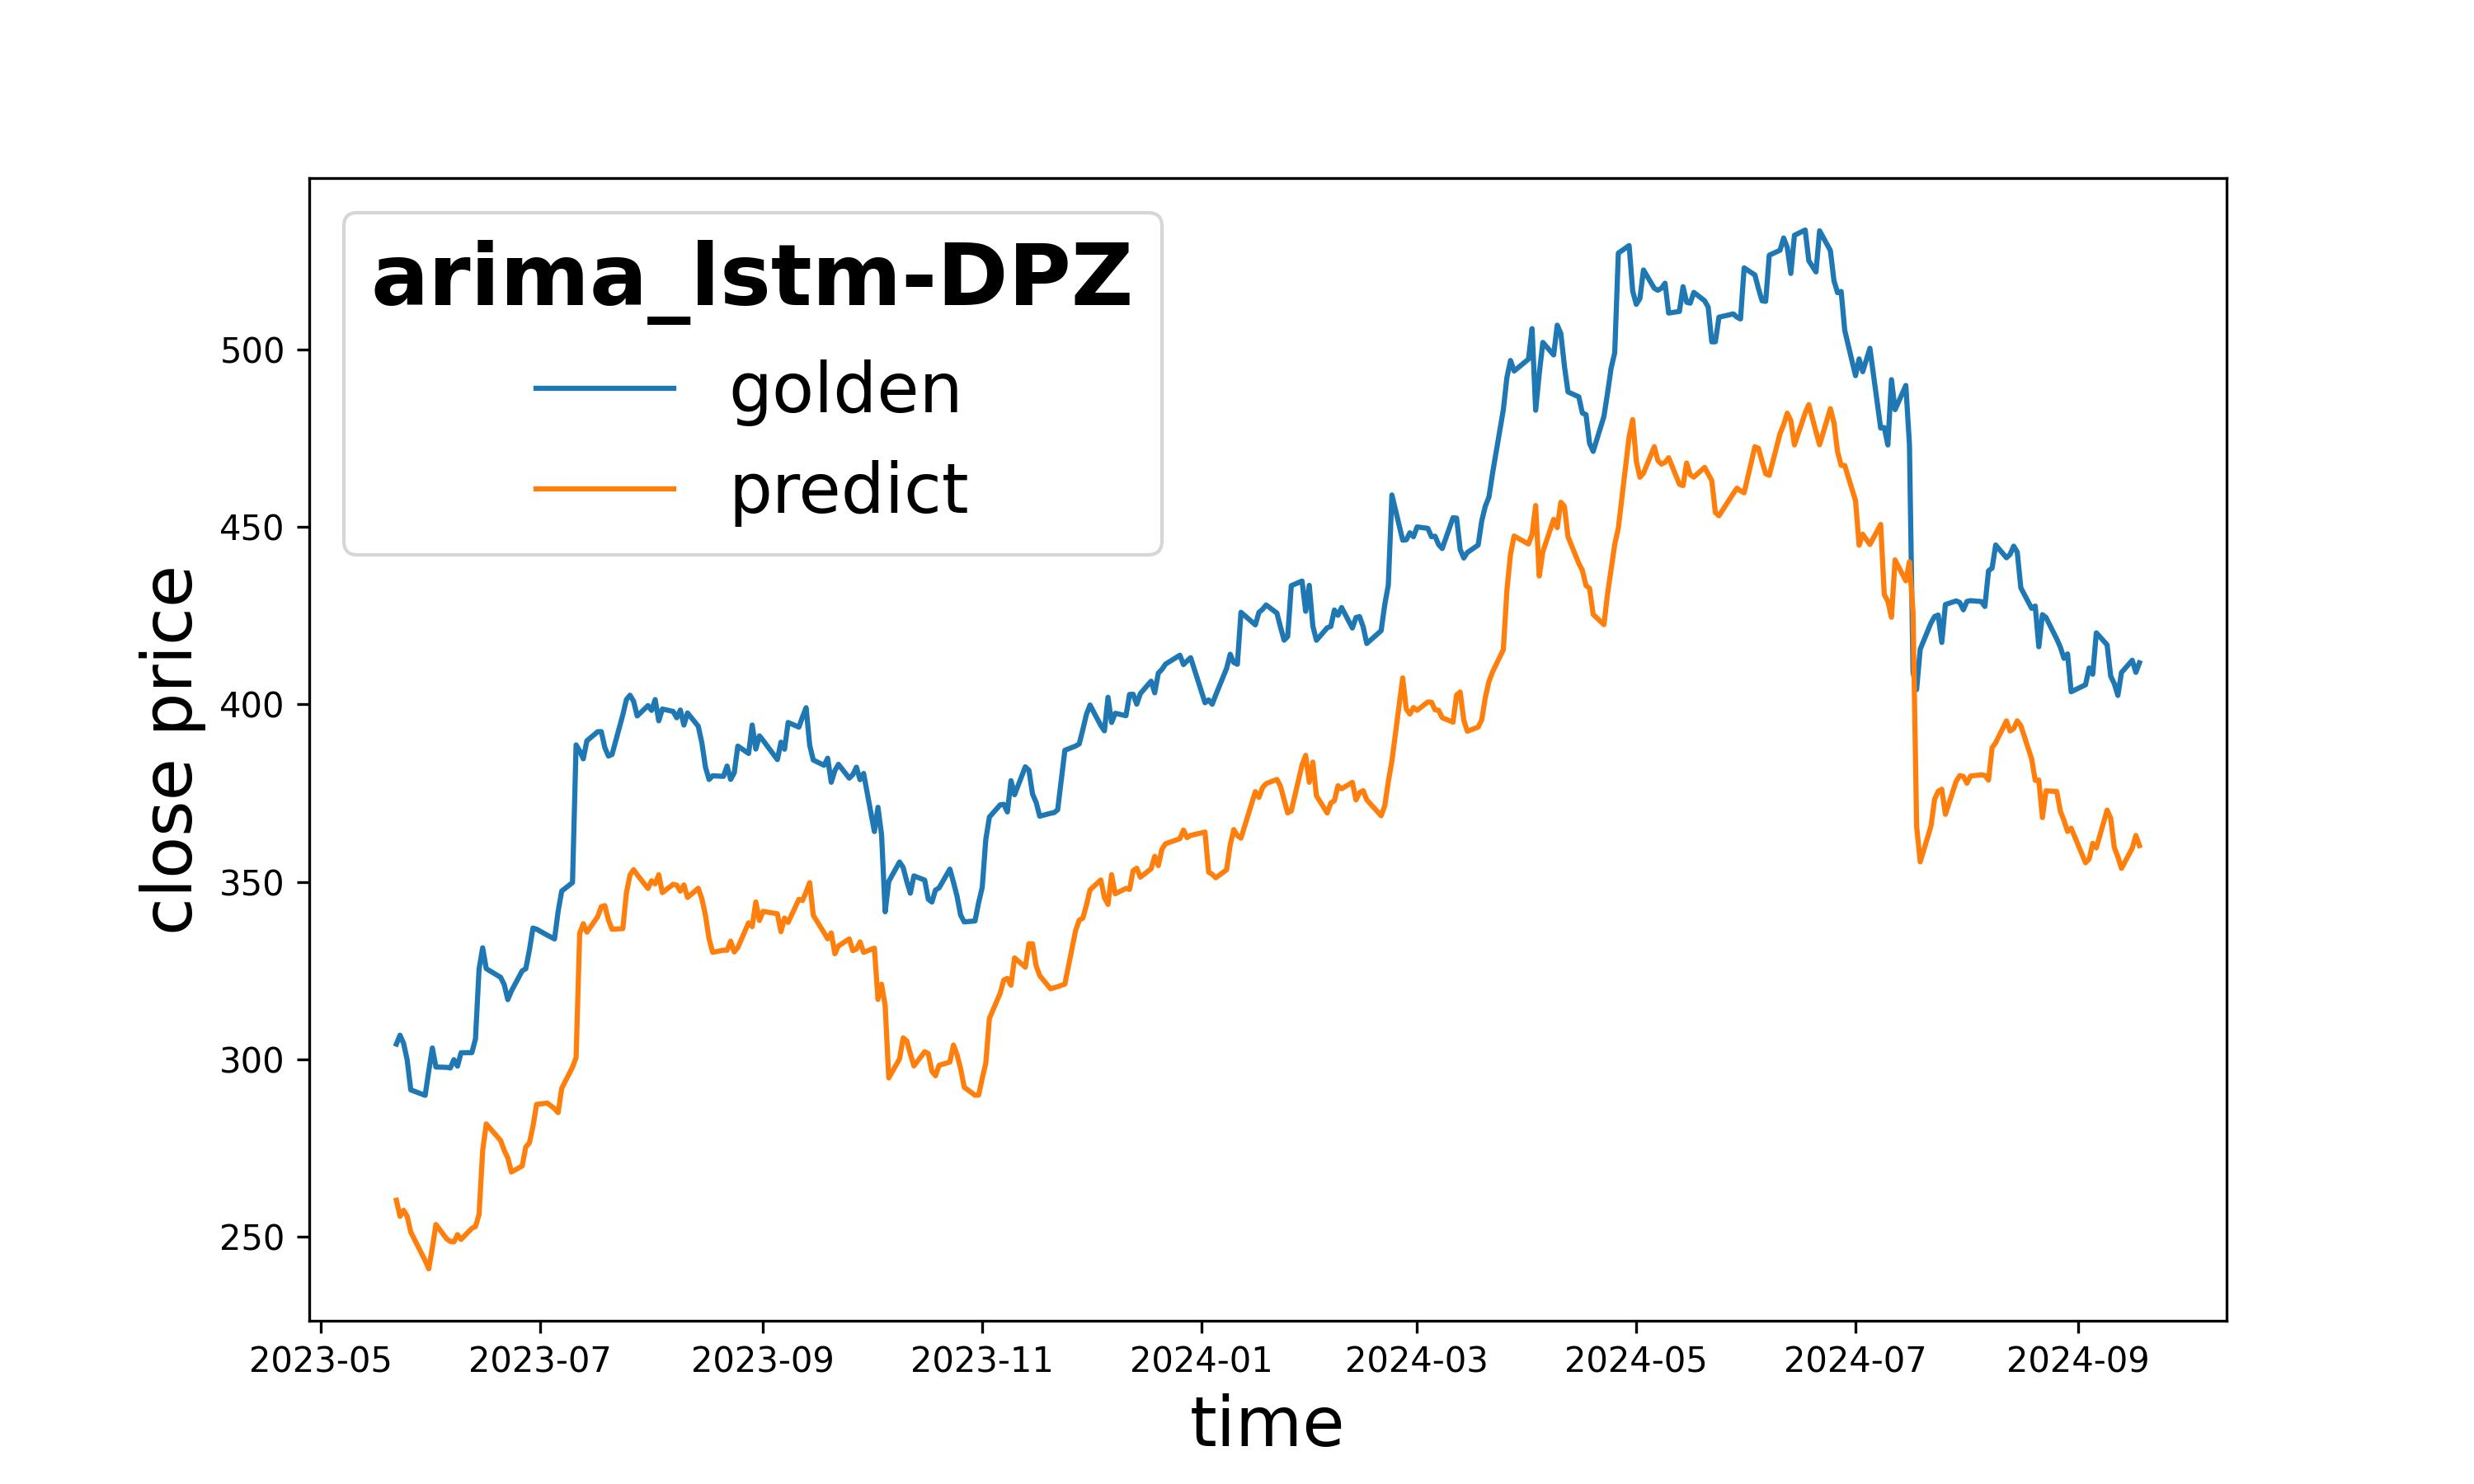
\includegraphics[width=\textwidth]{Result-Image/Result-Image3/02.DPZ/arima_lstm-DPZ.jpg}
%        \caption{ARIMA-LSTM}
%        \label{fig:image4}
%    \end{subfigure}
%    
%    \caption{DPZ}
%    \label{fig:2x2grid}
%\end{figure}
%
%%\subsection{MCD}
%\begin{figure}[ht]
%    \centering
%    \begin{subfigure}[b]{0.49\textwidth}
%        \centering
%        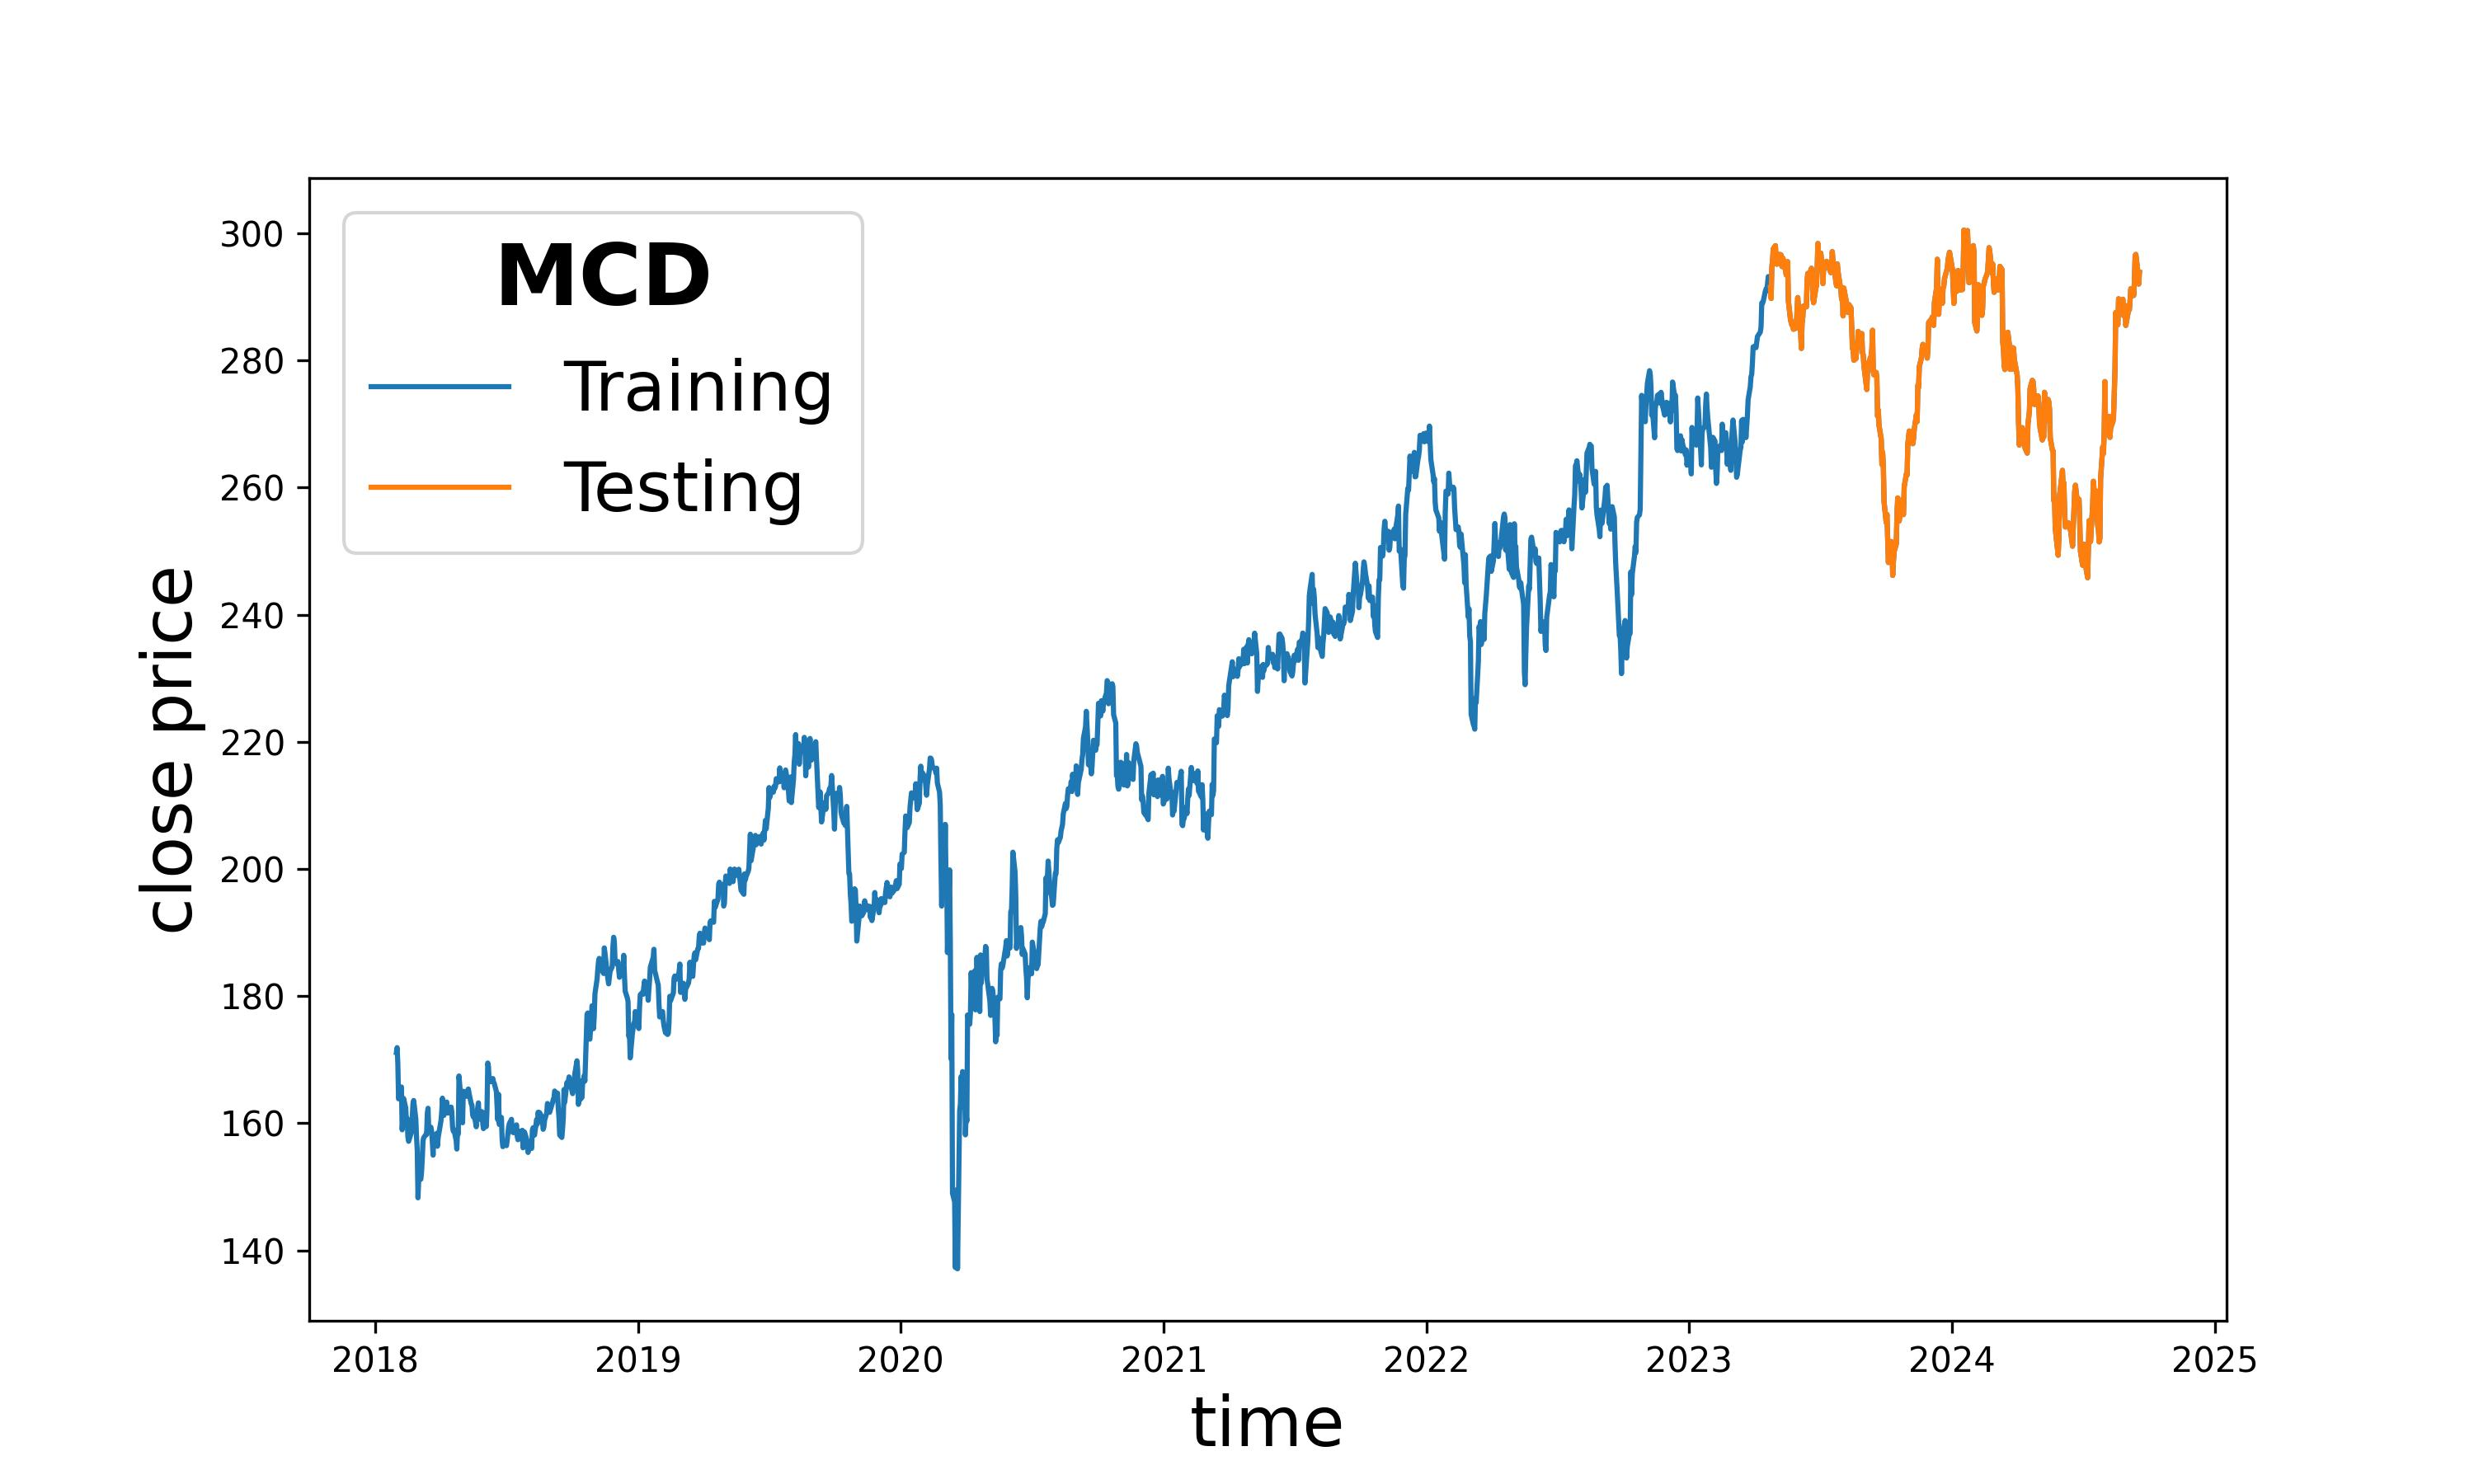
\includegraphics[width=\textwidth]{Result-Image/Result-Image3/03.MCD/MCD.jpg}
%        \caption{Training/Testing}
%        \label{fig:image1}
%    \end{subfigure}
%    
%    % 첫 번째 행
%    \begin{subfigure}[b]{0.49\textwidth}
%        \centering
%        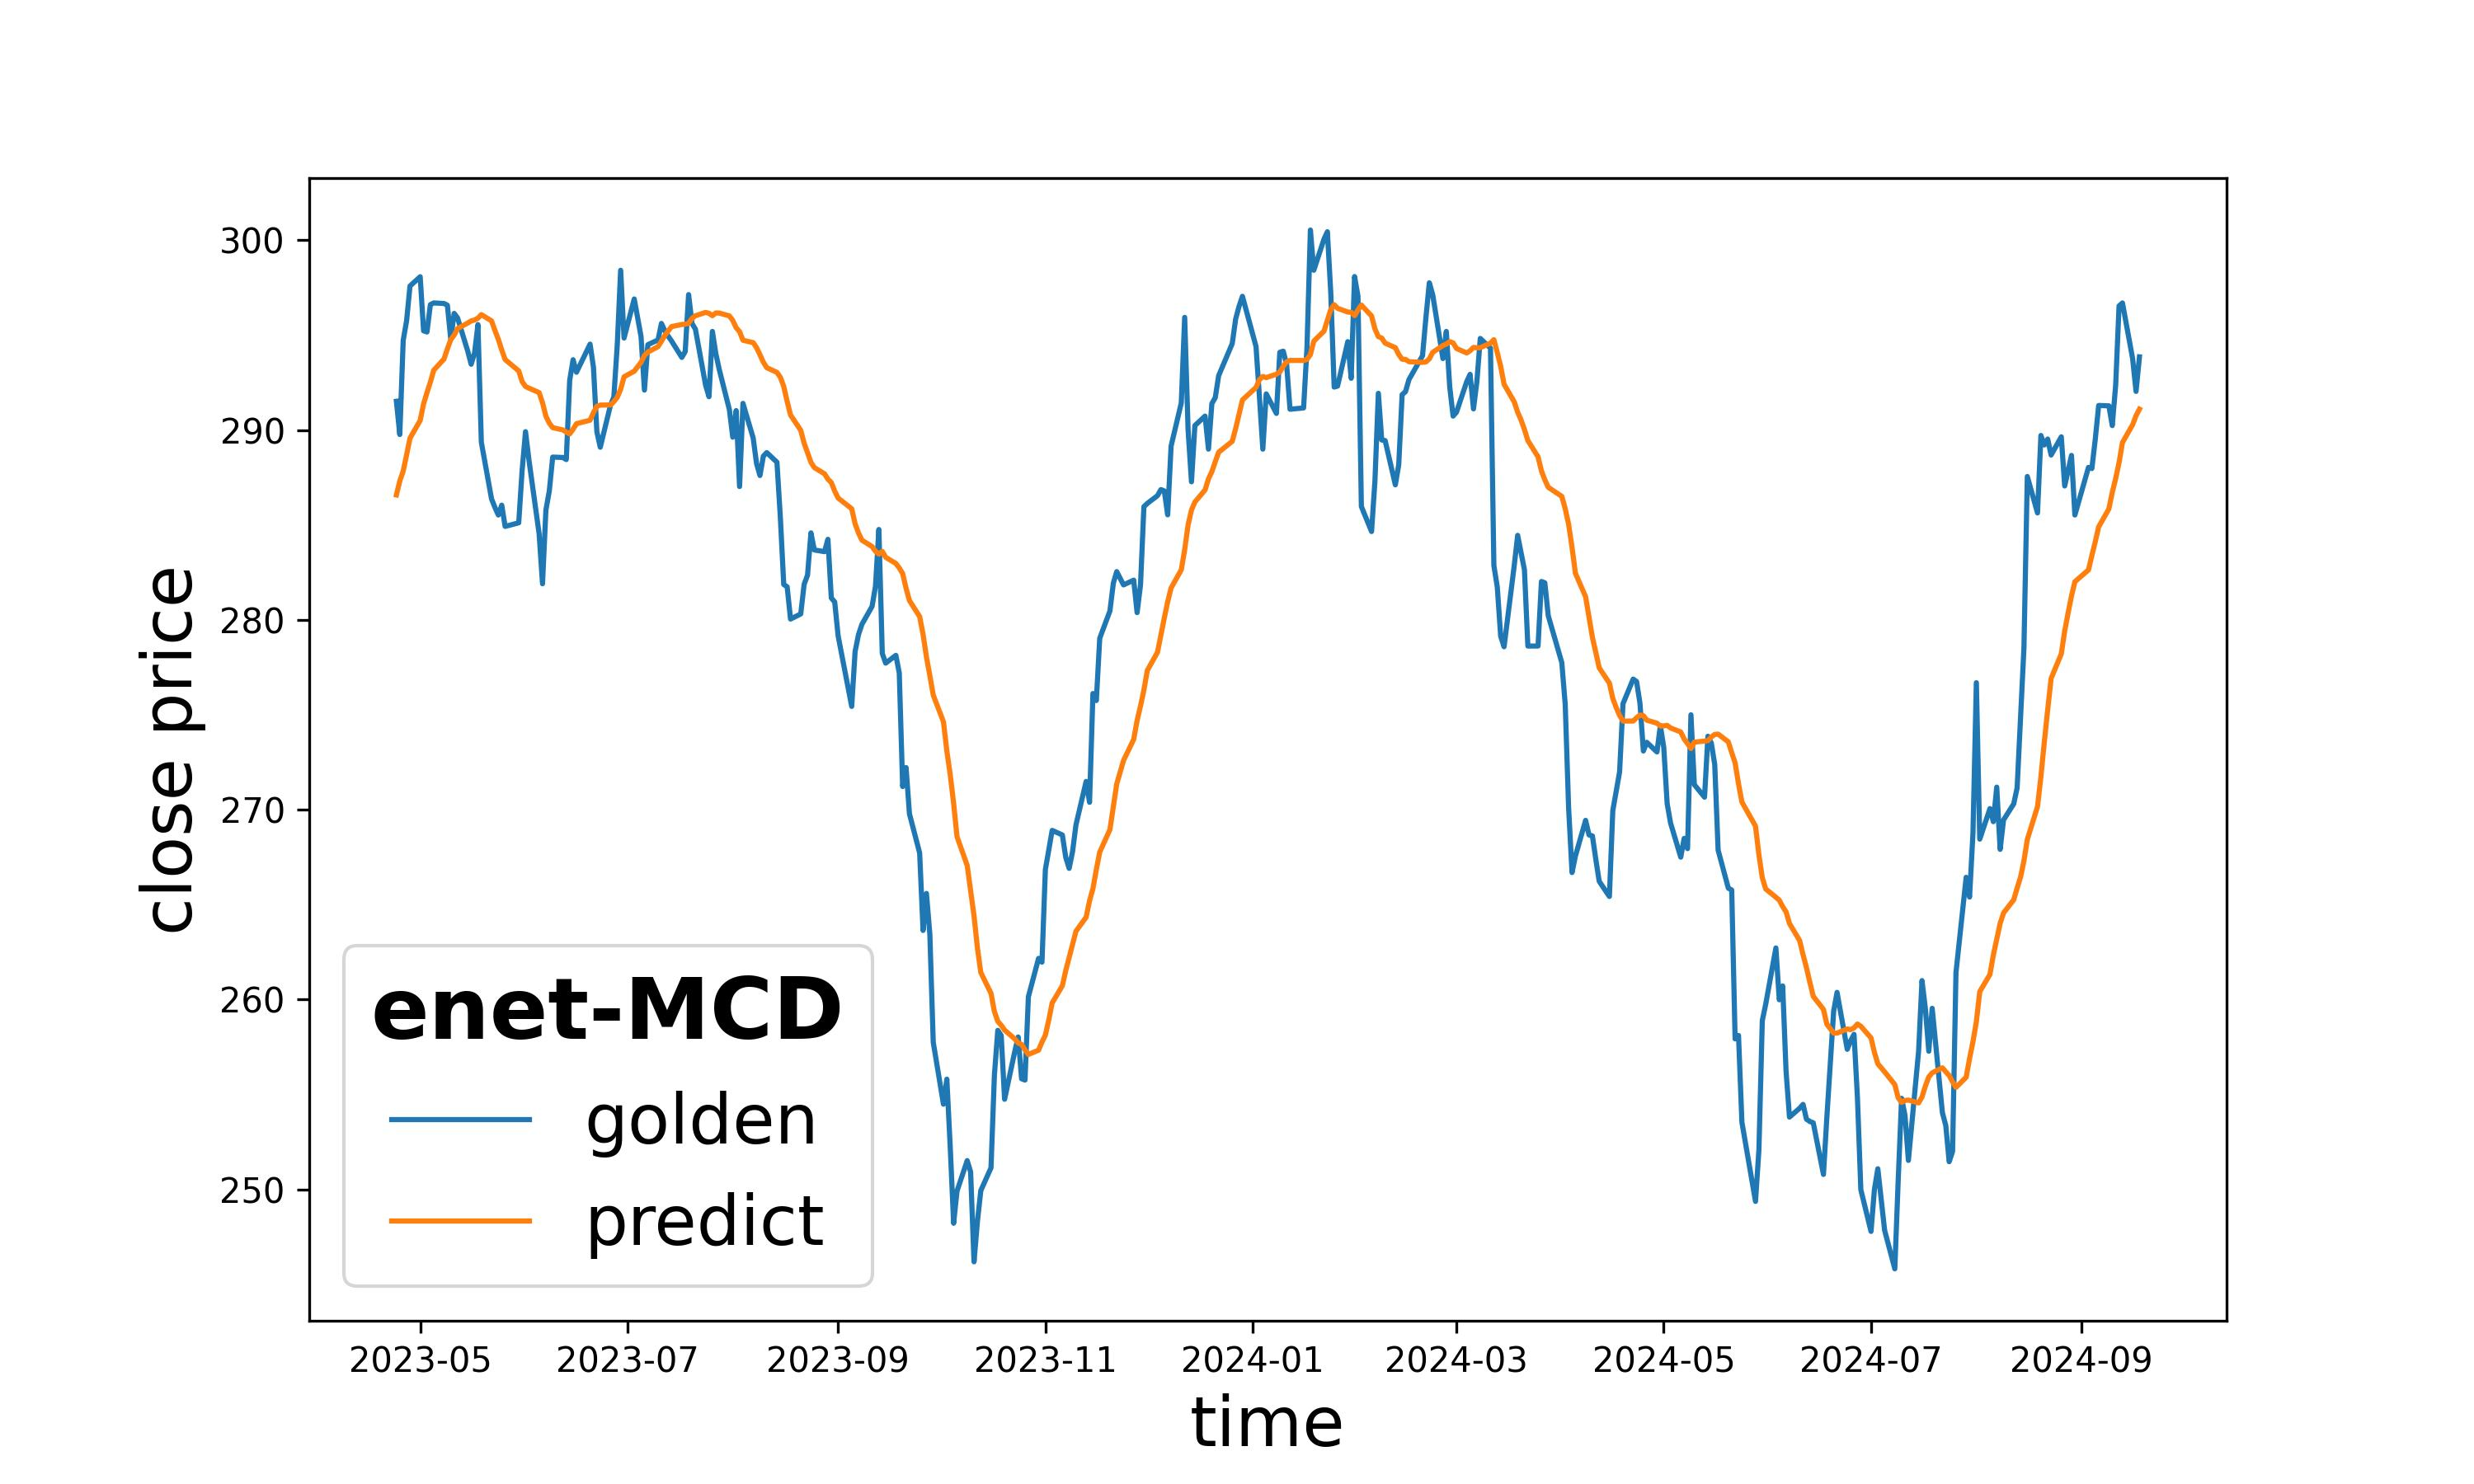
\includegraphics[width=\textwidth]{Result-Image/Result-Image3/03.MCD/enet-MCD.jpg}
%        \caption{Enet}
%        \label{fig:image1}
%    \end{subfigure}
%    \hfill
%    \begin{subfigure}[b]{0.49\textwidth}
%        \centering
%        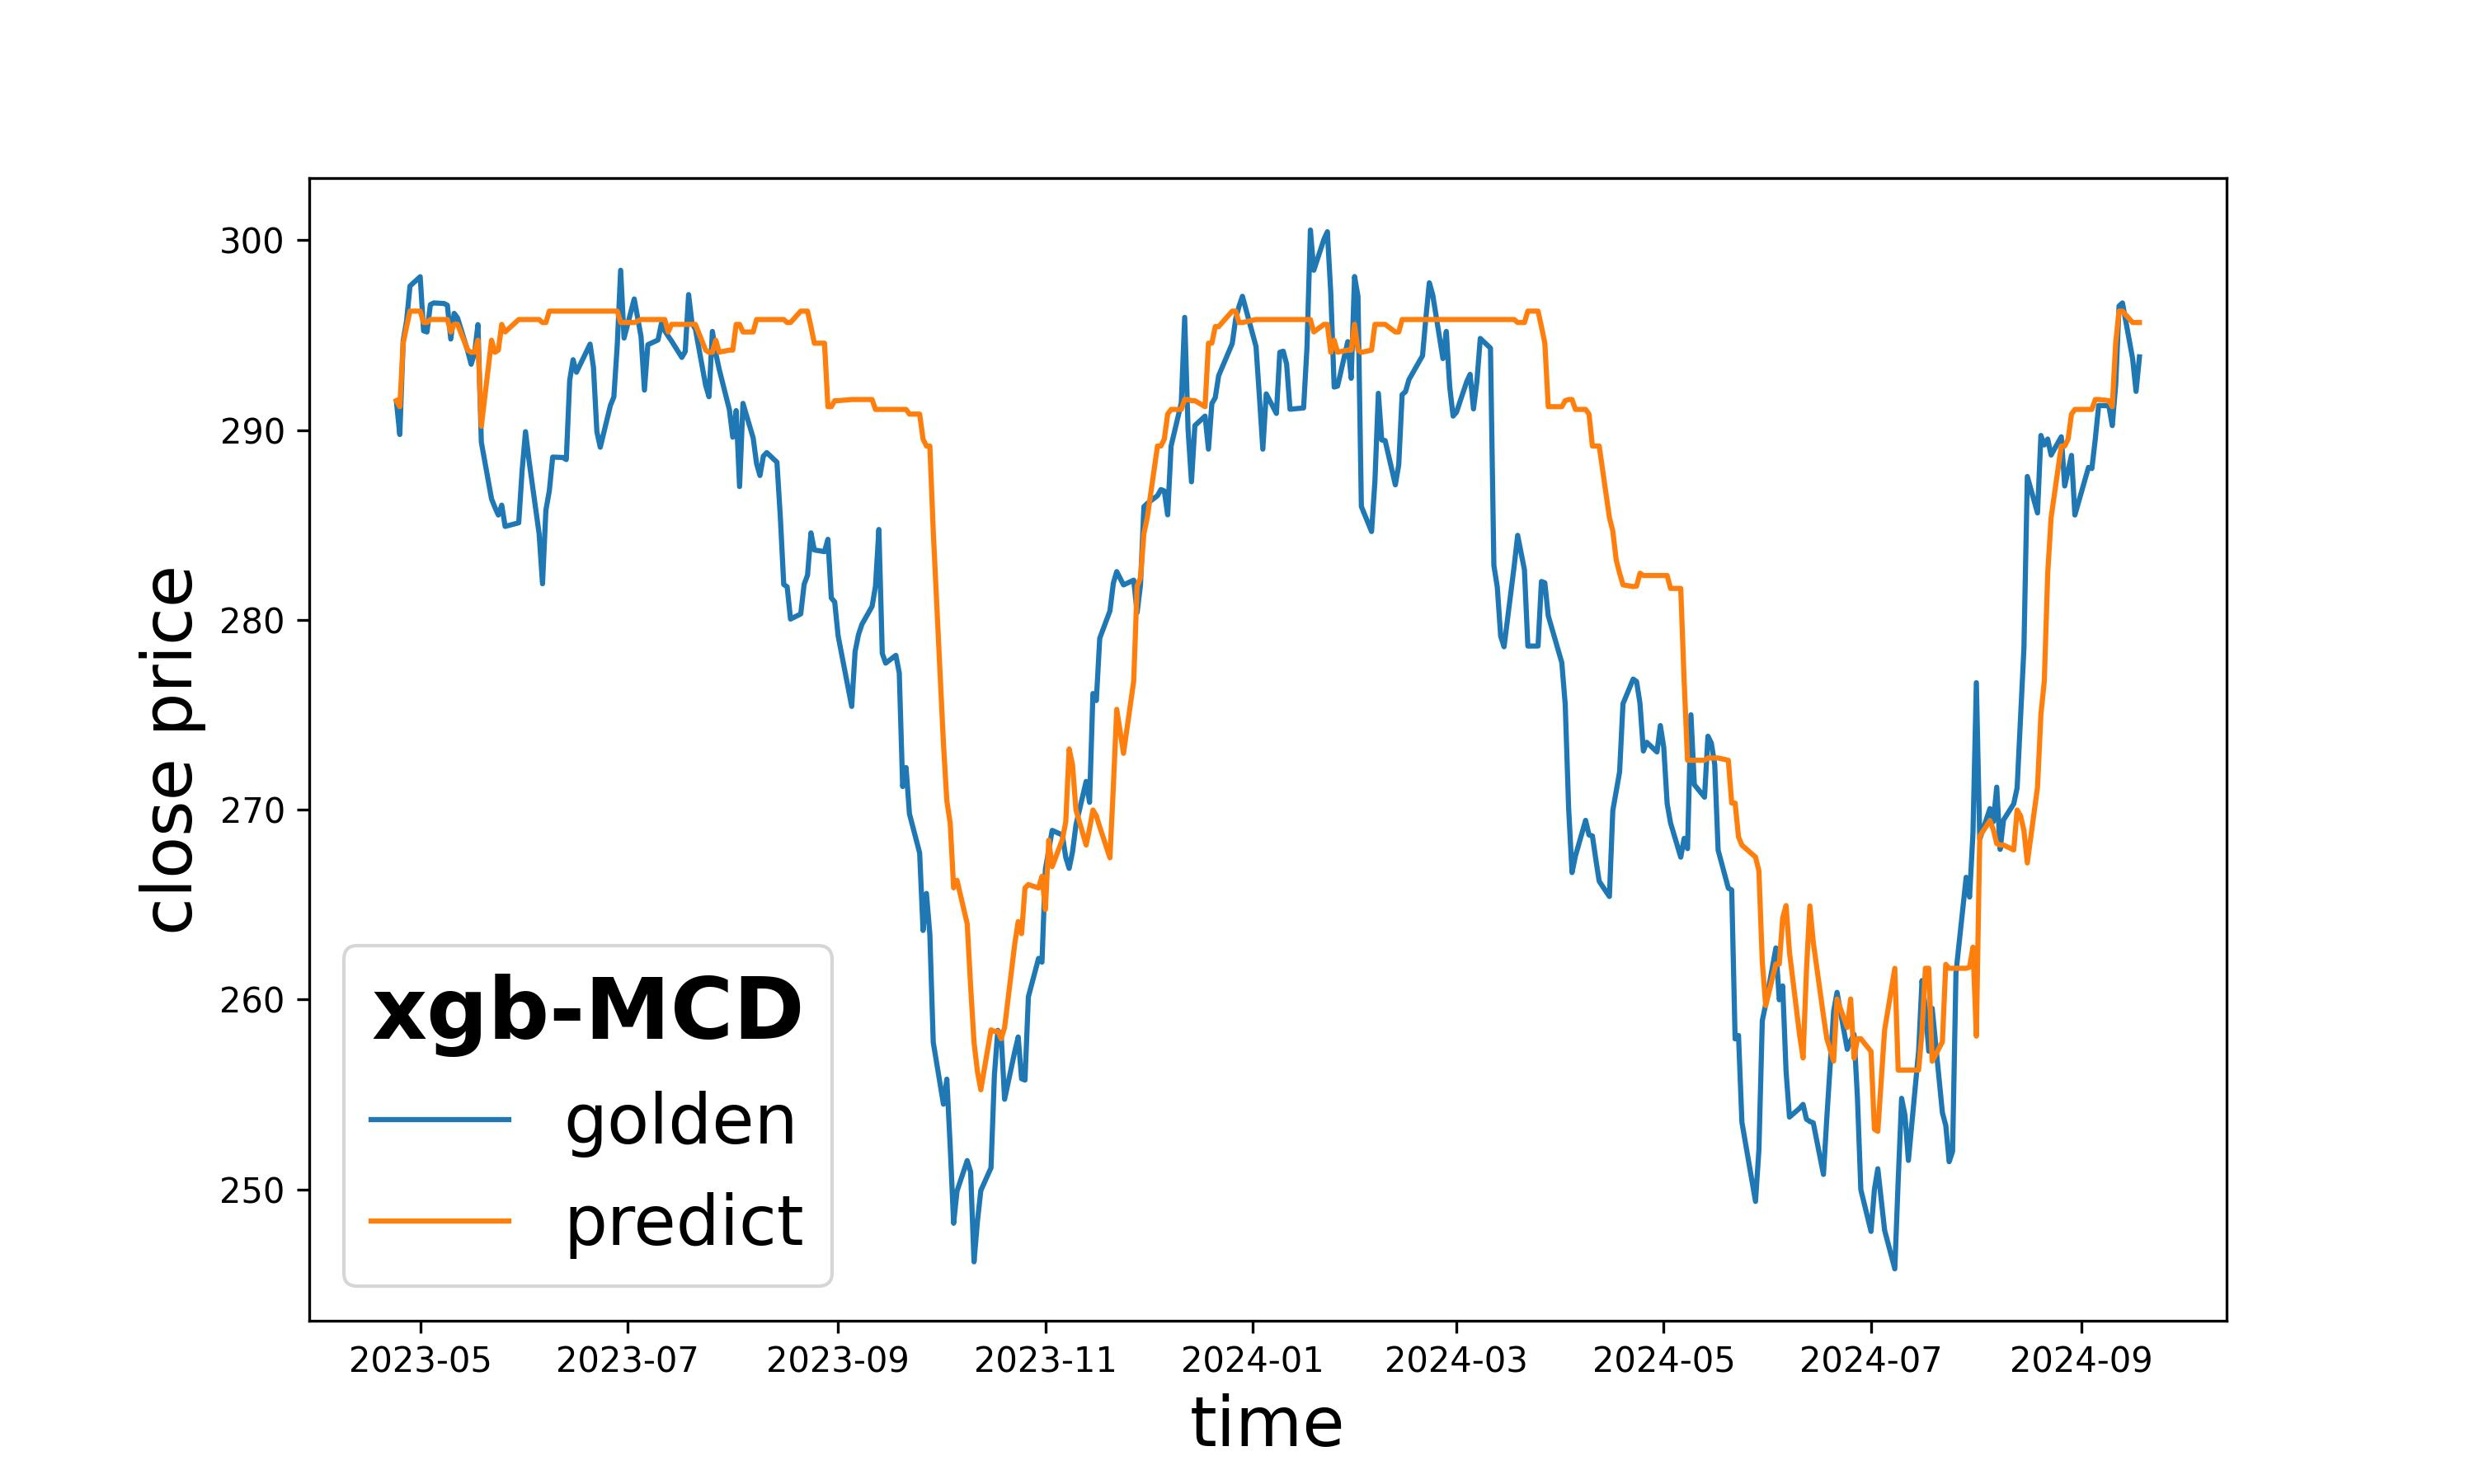
\includegraphics[width=\textwidth]{Result-Image/Result-Image3/03.MCD/xgb-MCD.jpg}
%        \caption{XGBoost}
%        \label{fig:image2}
%    \end{subfigure}
%    
%    % 두 번째 행
%    \vskip\baselineskip
%    \begin{subfigure}[b]{0.49\textwidth}
%        \centering
%        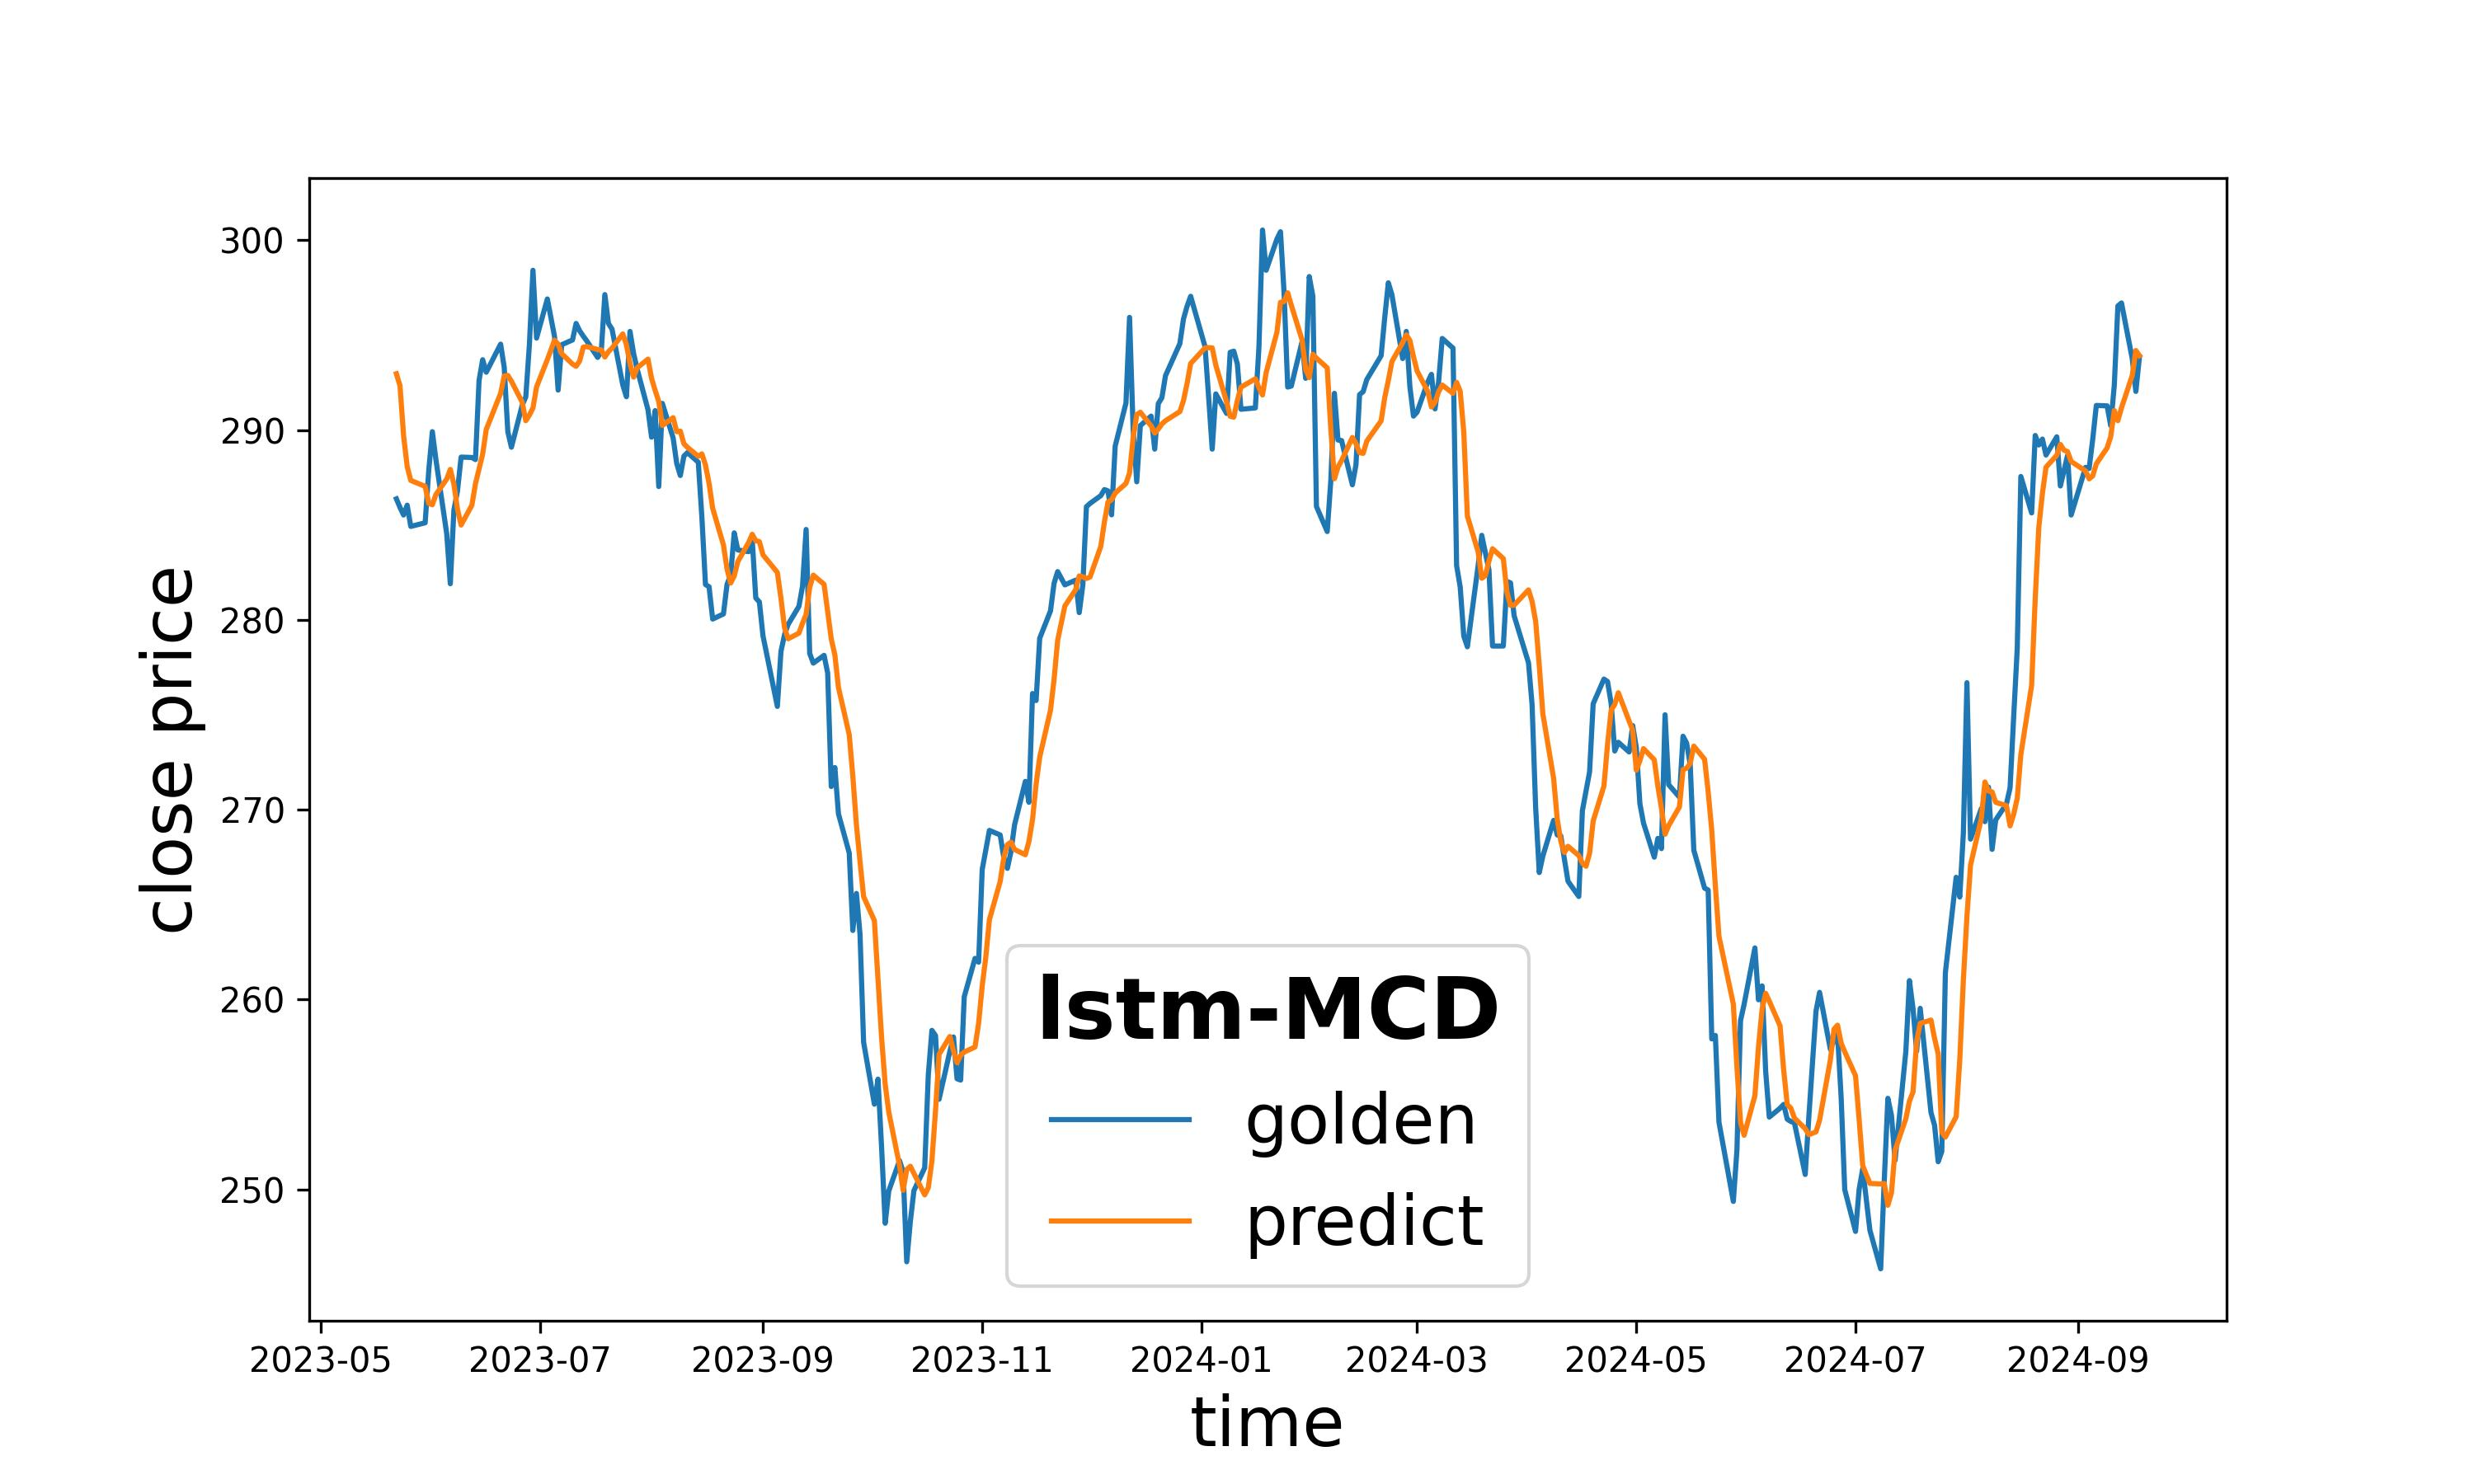
\includegraphics[width=\textwidth]{Result-Image/Result-Image3/03.MCD/lstm-MCD.jpg}
%        \caption{LSTM}
%        \label{fig:image3}
%    \end{subfigure}
%    \hfill
%    \begin{subfigure}[b]{0.49\textwidth}
%        \centering
%        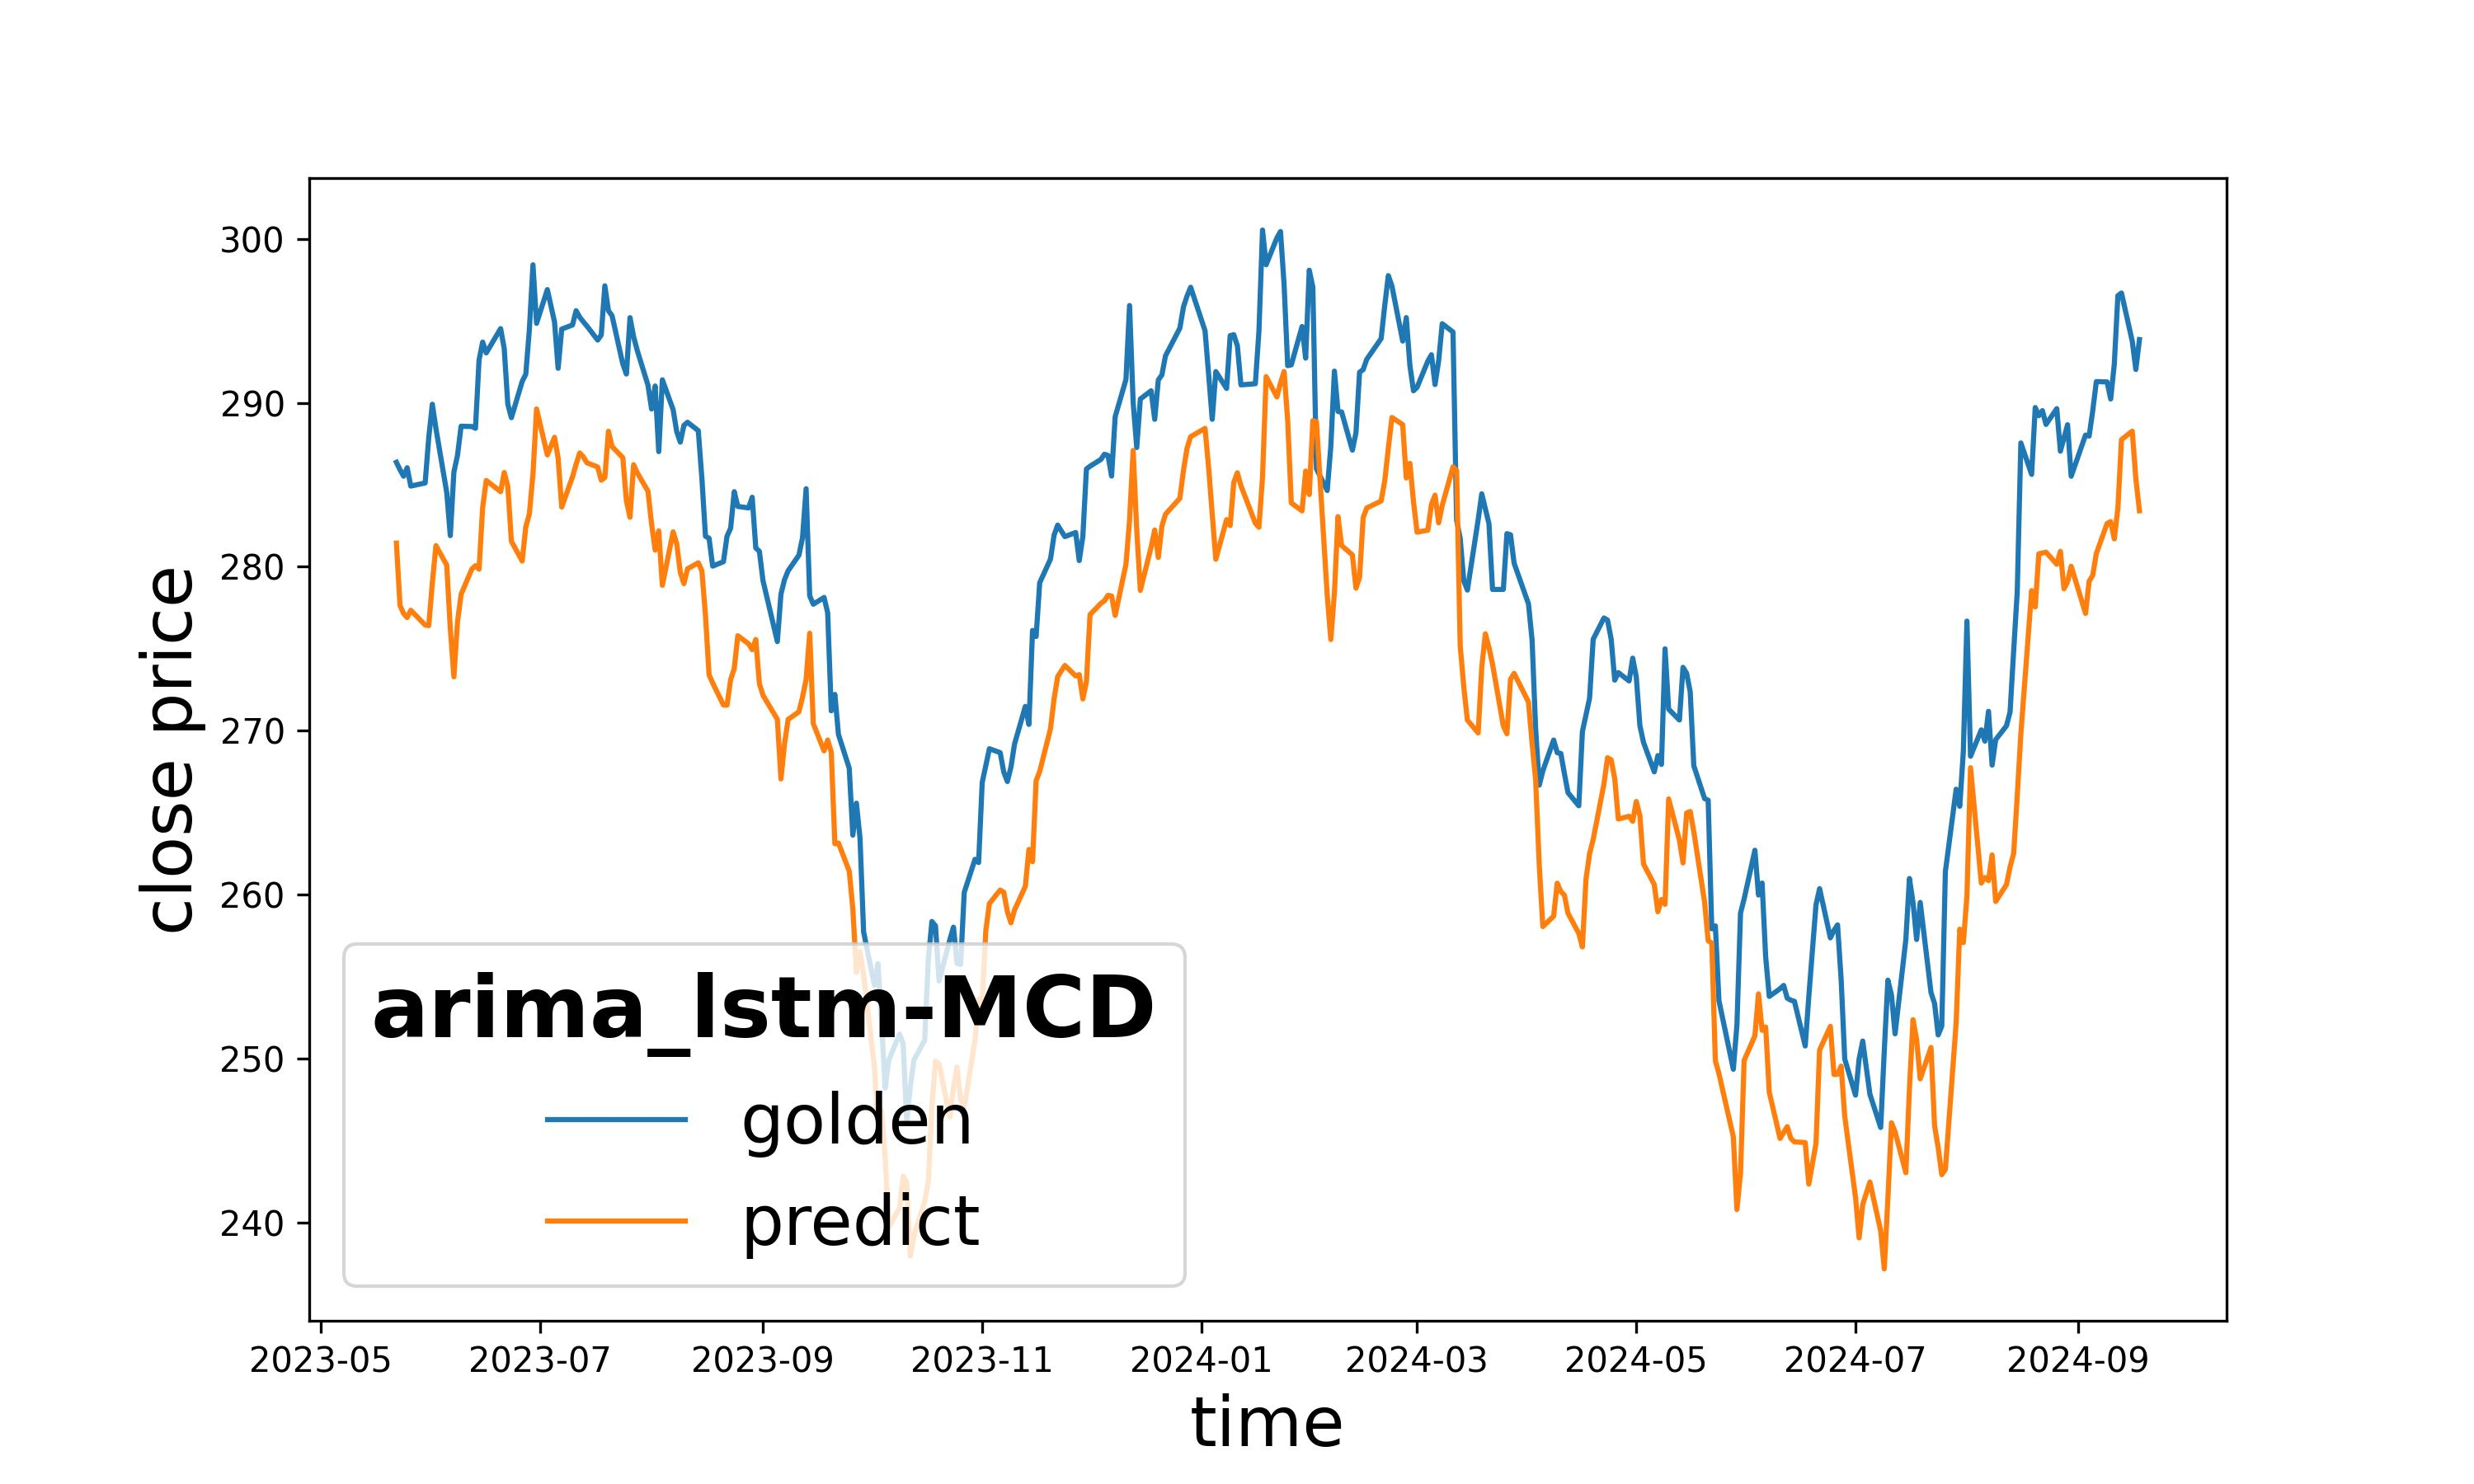
\includegraphics[width=\textwidth]{Result-Image/Result-Image3/03.MCD/arima_lstm-MCD.jpg}
%        \caption{ARIMA-LSTM}
%        \label{fig:image4}
%    \end{subfigure}
%    
%    \caption{MCD}
%    \label{fig:2x2grid}
%\end{figure}
%
%\subsection{QSR}
\begin{figure}[ht]
    \centering
    \begin{subfigure}[b]{0.49\textwidth}
        \centering
        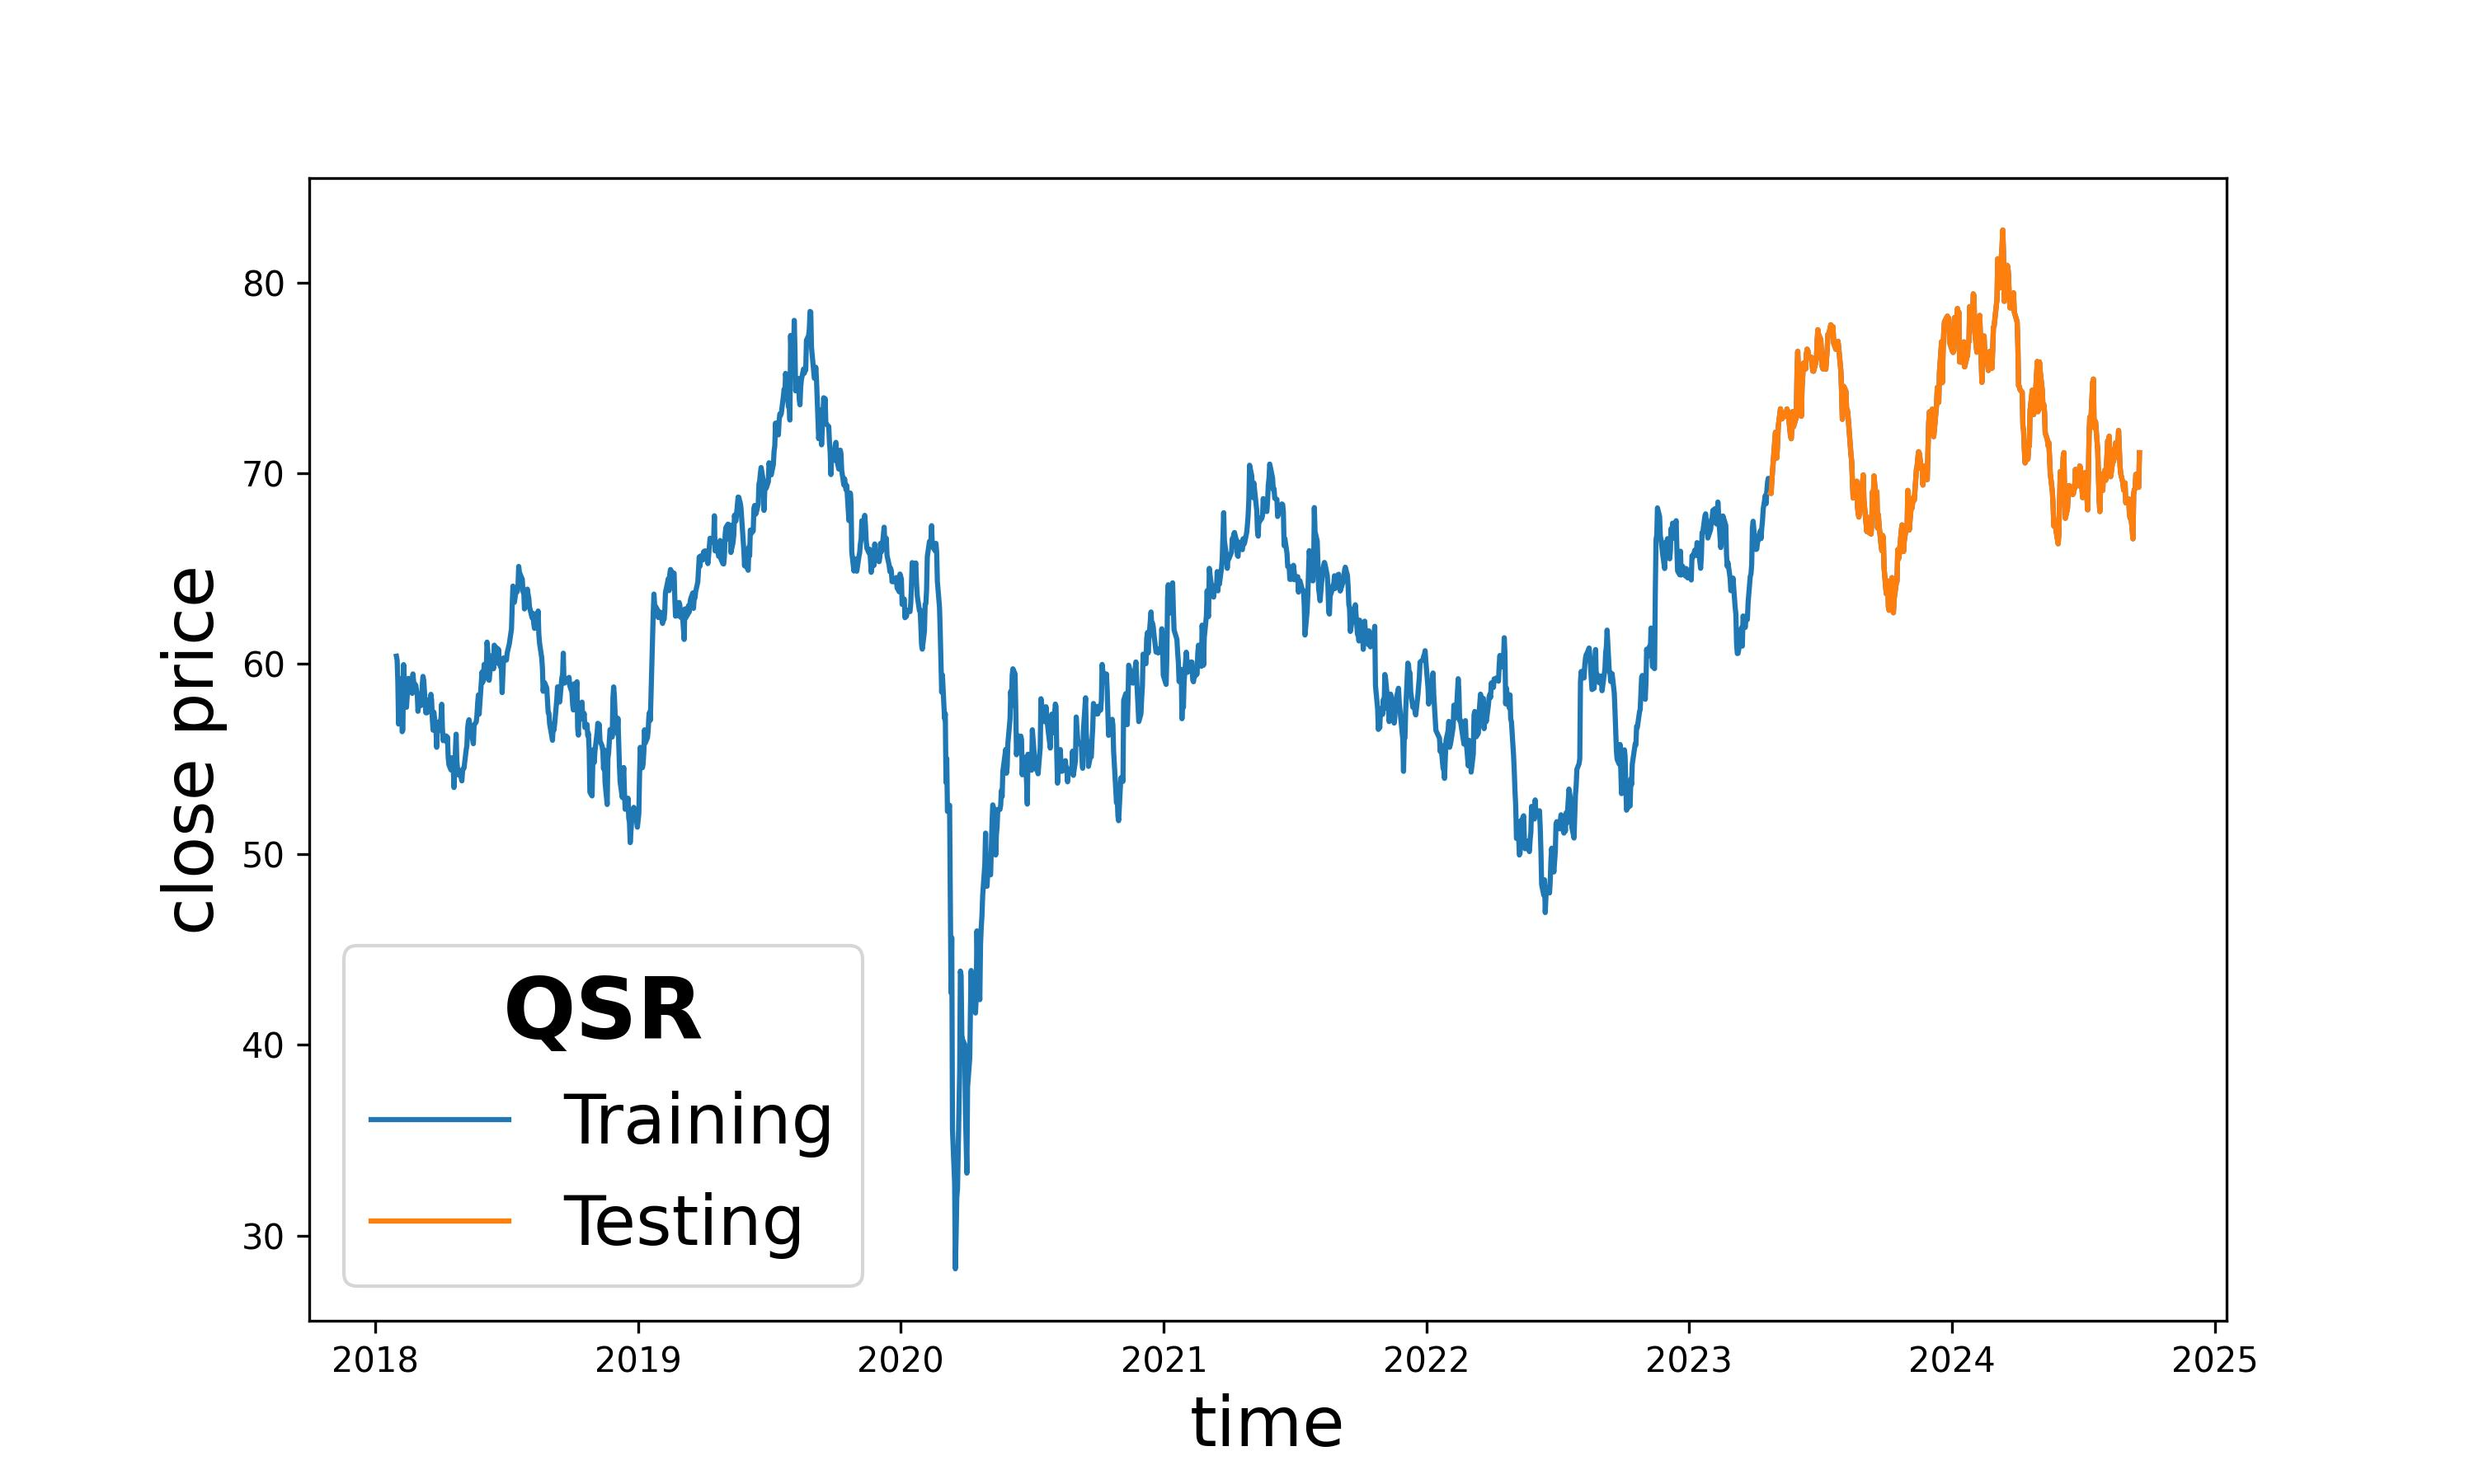
\includegraphics[width=\textwidth]{Result-Image/Result-Image3/04.QSR/QSR.jpg}
        \caption{Training/Testing}
        \label{fig:image1}
    \end{subfigure}

    
    % 첫 번째 행
    \begin{subfigure}[b]{0.49\textwidth}
        \centering
        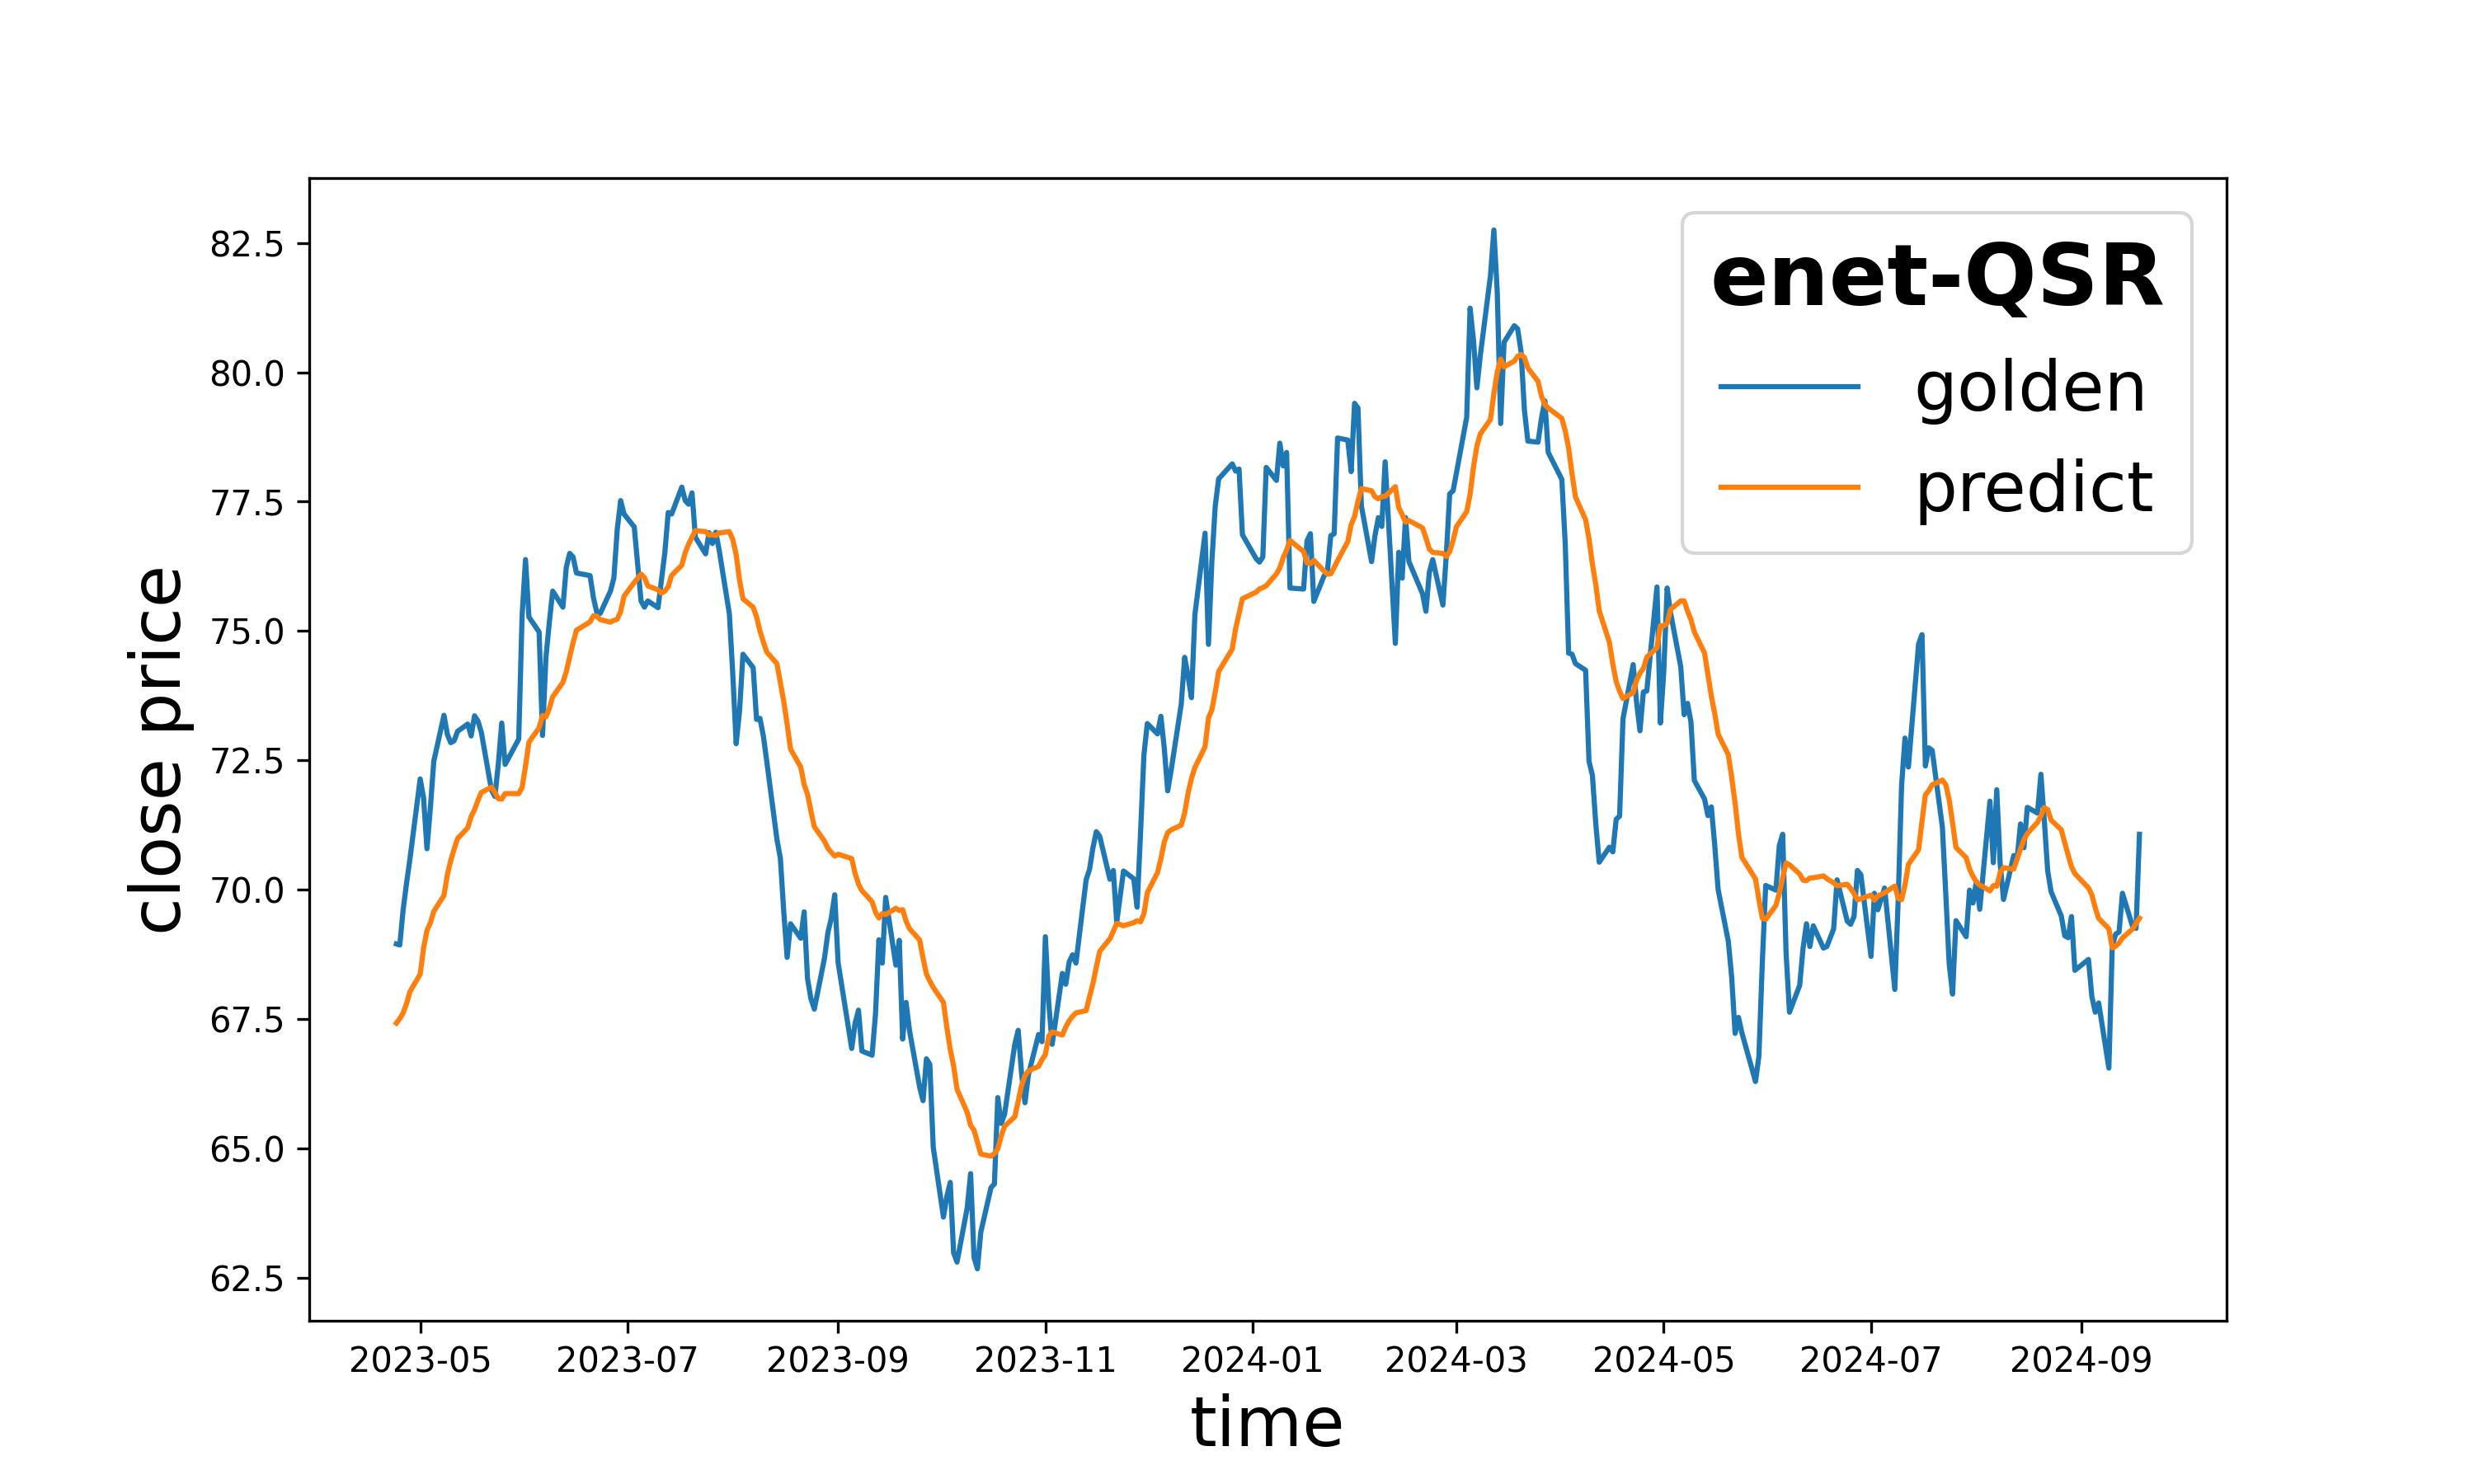
\includegraphics[width=\textwidth]{Result-Image/Result-Image3/04.QSR/enet-QSR.jpg}
        \caption{Enet}
        \label{fig:image1}
    \end{subfigure}
    \hfill
    \begin{subfigure}[b]{0.49\textwidth}
        \centering
        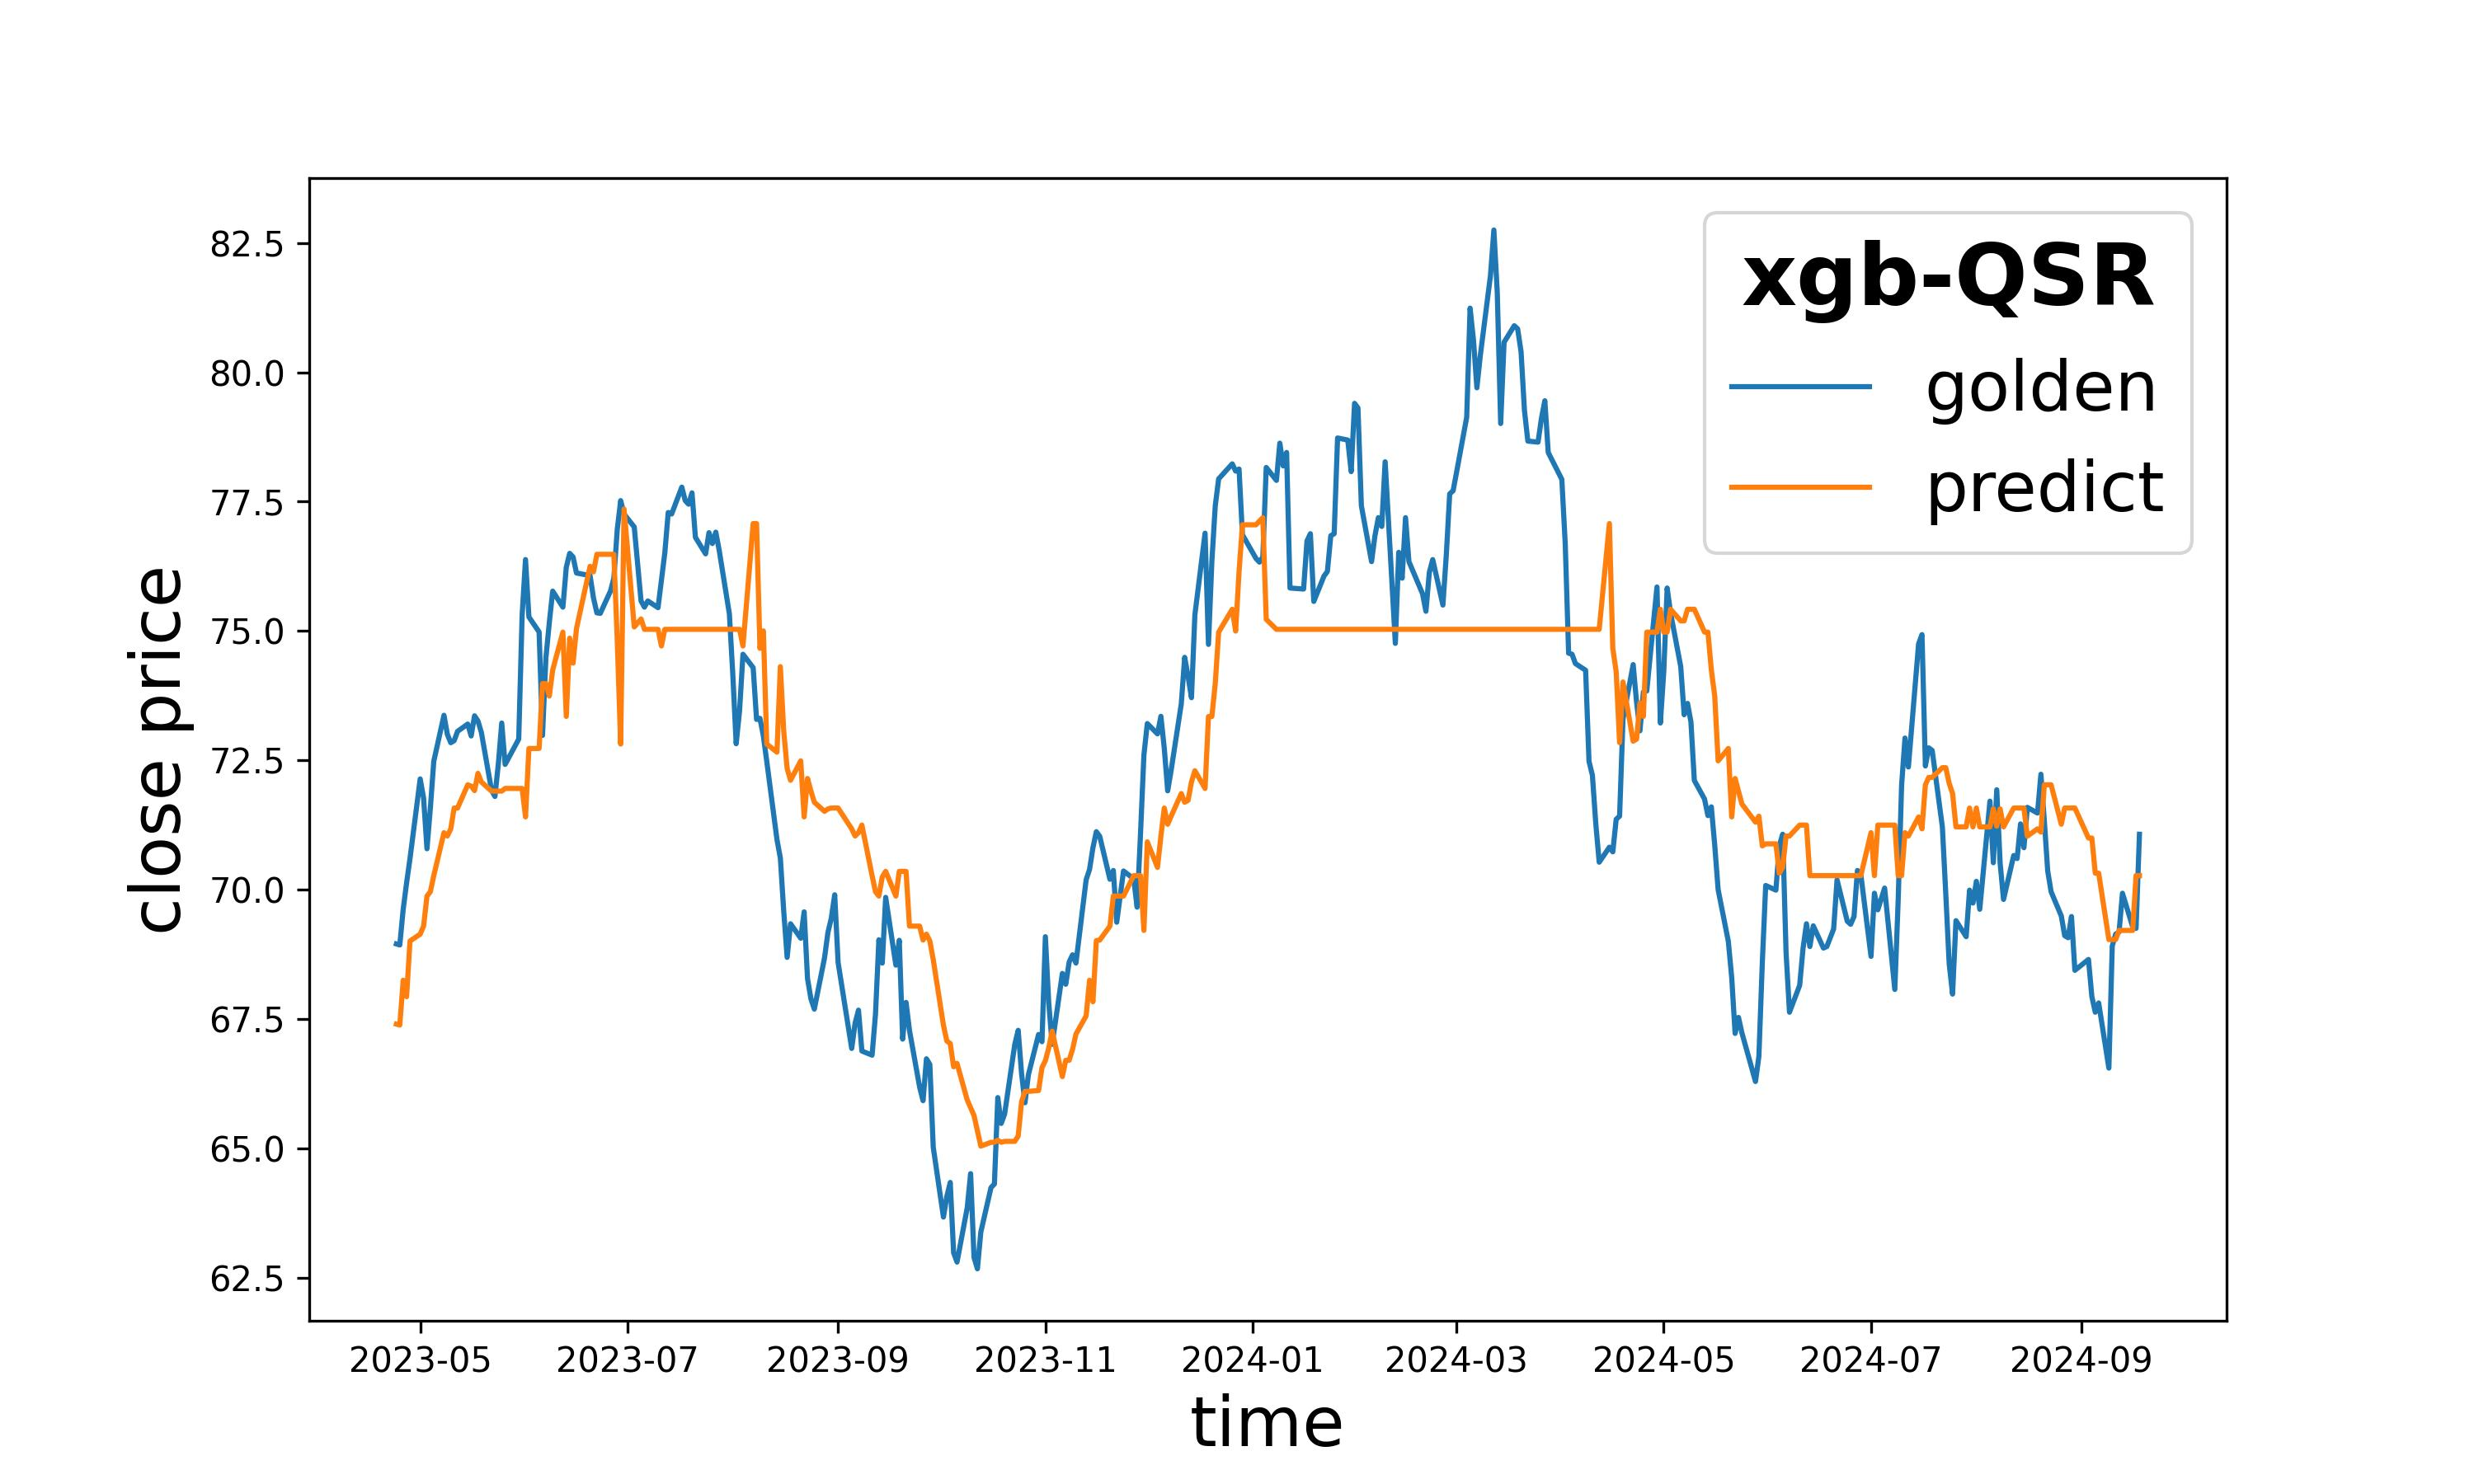
\includegraphics[width=\textwidth]{Result-Image/Result-Image3/04.QSR/xgb-QSR.jpg}
        \caption{XGBoost}
        \label{fig:image2}
    \end{subfigure}
    
    % 두 번째 행
    \vskip\baselineskip
    \begin{subfigure}[b]{0.49\textwidth}
        \centering
        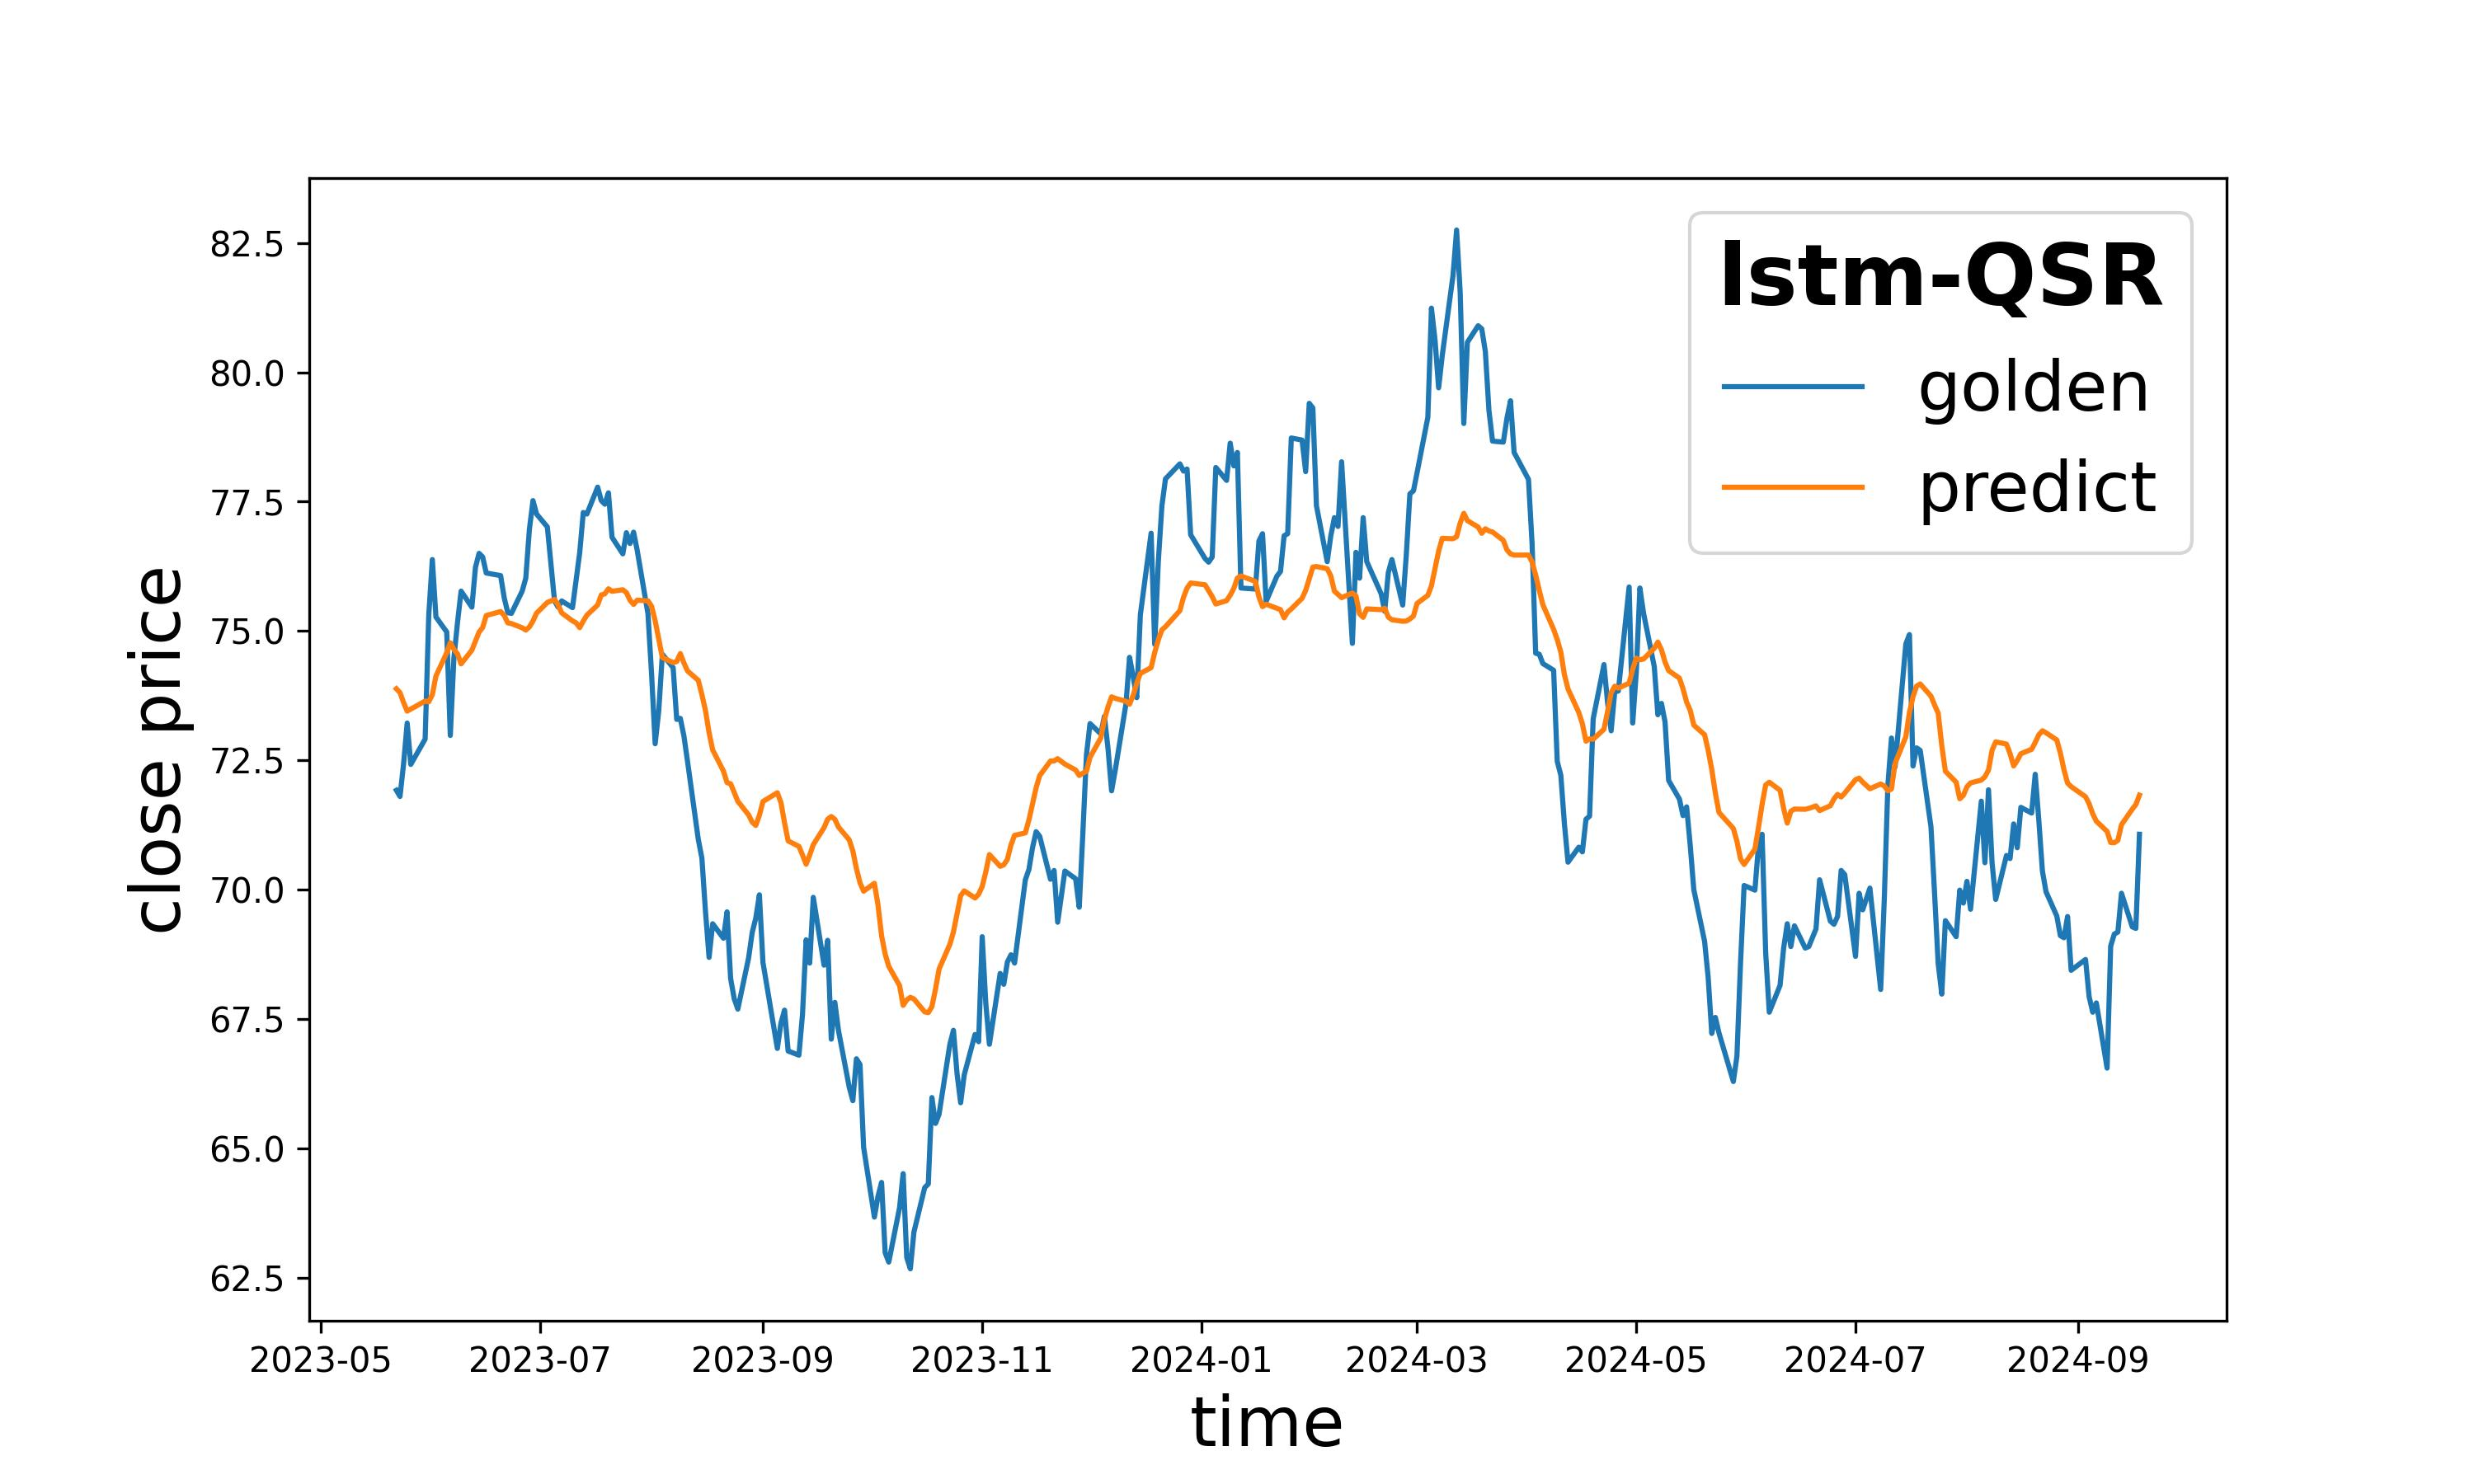
\includegraphics[width=\textwidth]{Result-Image/Result-Image3/04.QSR/lstm-QSR.jpg}
        \caption{LSTM}
        \label{fig:image3}
    \end{subfigure}
    \hfill
    \begin{subfigure}[b]{0.49\textwidth}
        \centering
        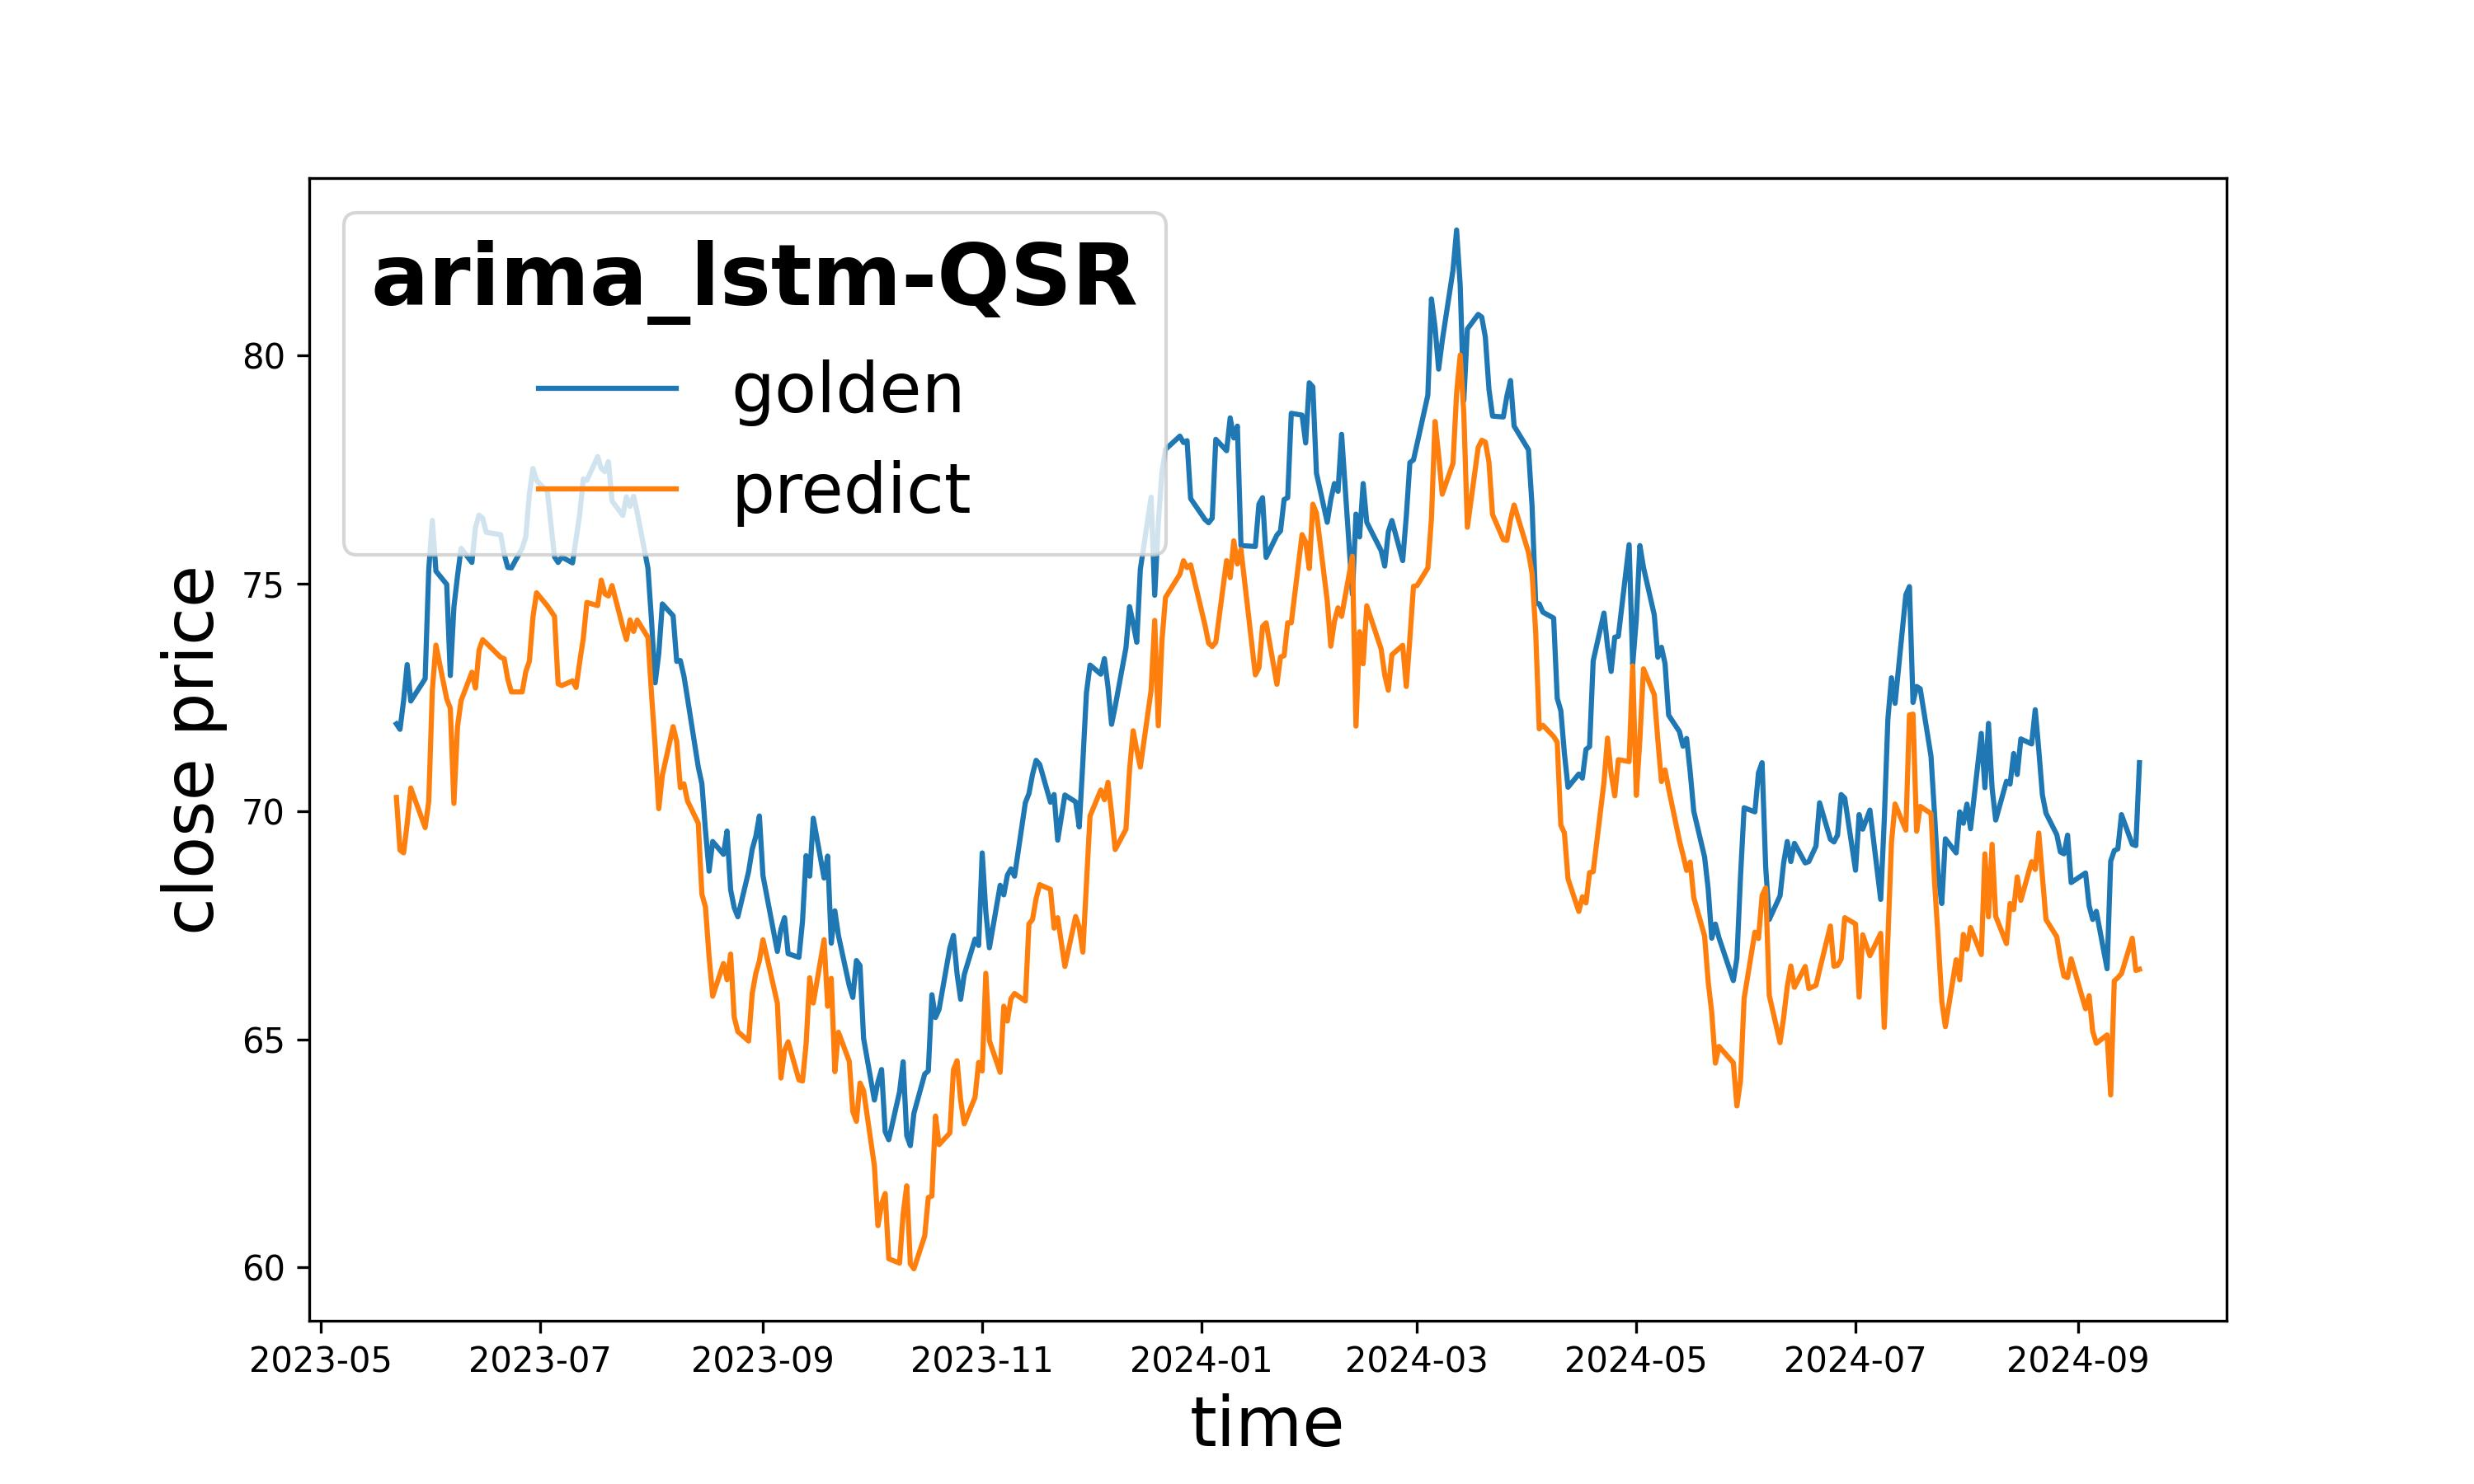
\includegraphics[width=\textwidth]{Result-Image/Result-Image3/04.QSR/arima_lstm-QSR.jpg}
        \caption{ARIMA-LSTM}
        \label{fig:image4}
    \end{subfigure}
    
    \caption{QSR}
    \label{fig:2x2grid}
\end{figure}

%\subsection{WEN}
\begin{figure}[ht]
    \centering
    \begin{subfigure}[b]{0.49\textwidth}
        \centering
        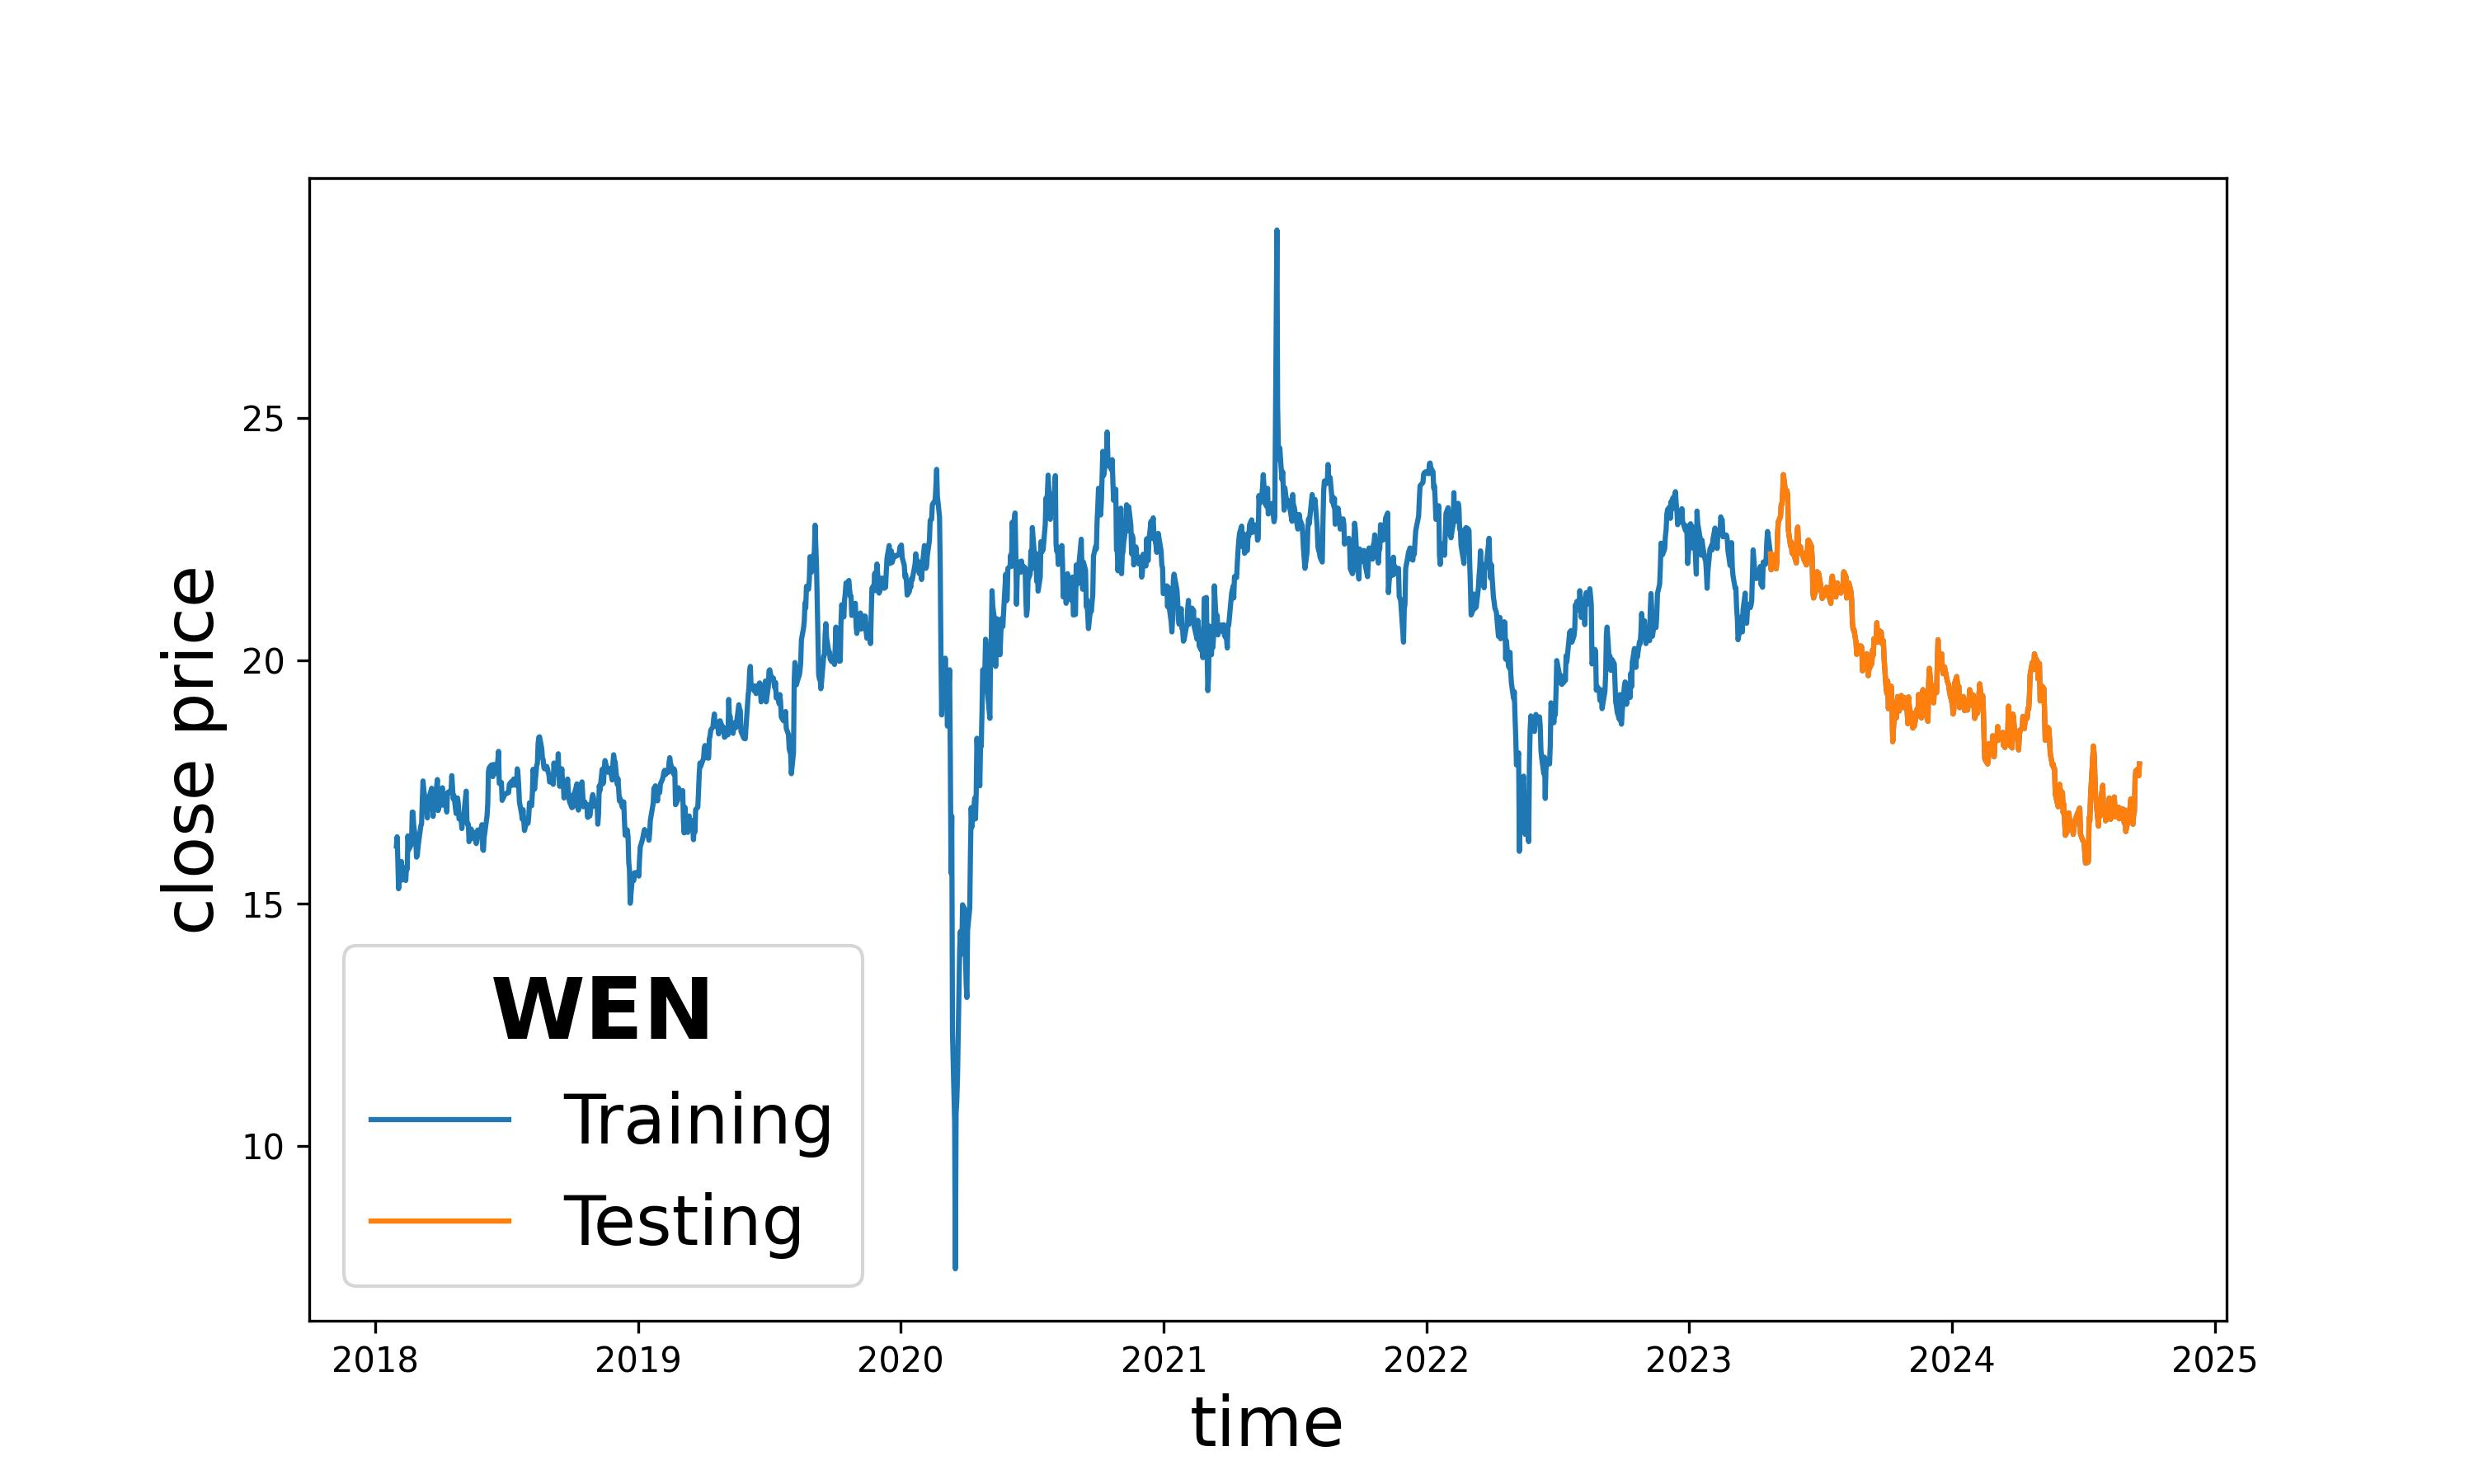
\includegraphics[width=\textwidth]{Result-Image/Result-Image3/05.WEN/WEN.jpg}
        \caption{Training/Testing}
        \label{fig:image1}
    \end{subfigure}
    
    % 첫 번째 행
    \begin{subfigure}[b]{0.49\textwidth}
        \centering
        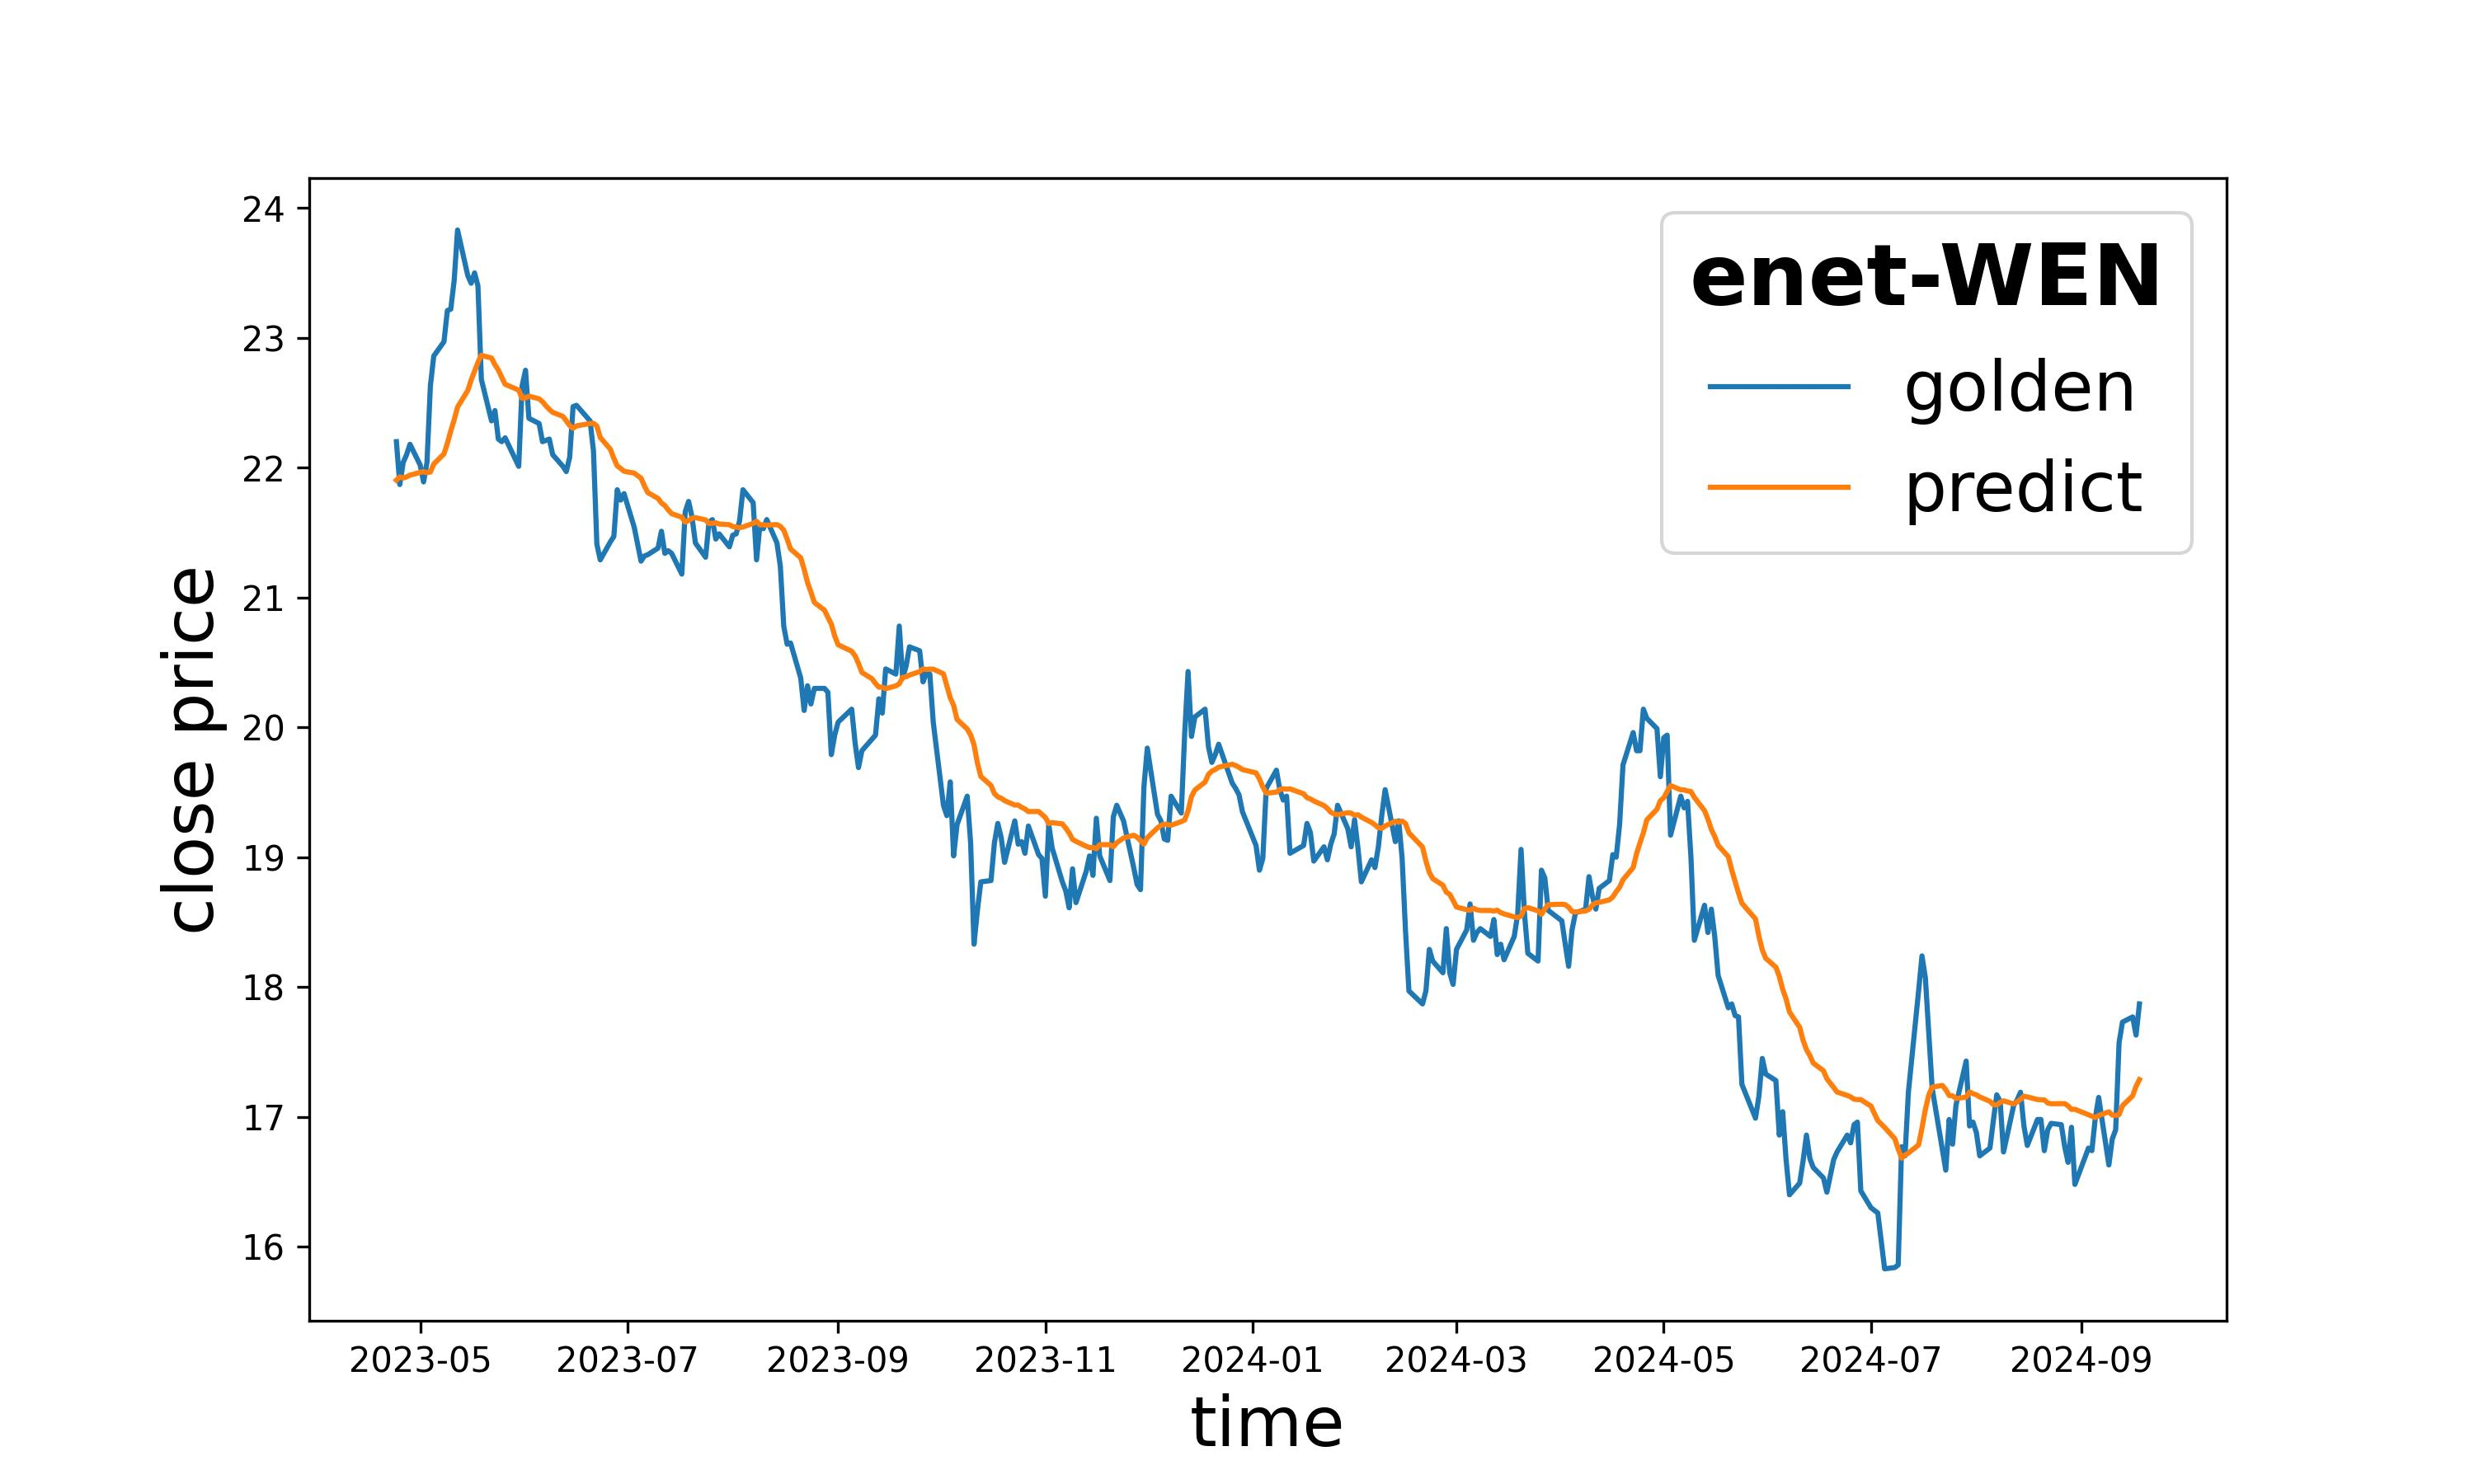
\includegraphics[width=\textwidth]{Result-Image/Result-Image3/05.WEN/enet-WEN.jpg}
        \caption{Enet}
        \label{fig:image1}
    \end{subfigure}
    \hfill
    \begin{subfigure}[b]{0.49\textwidth}
        \centering
        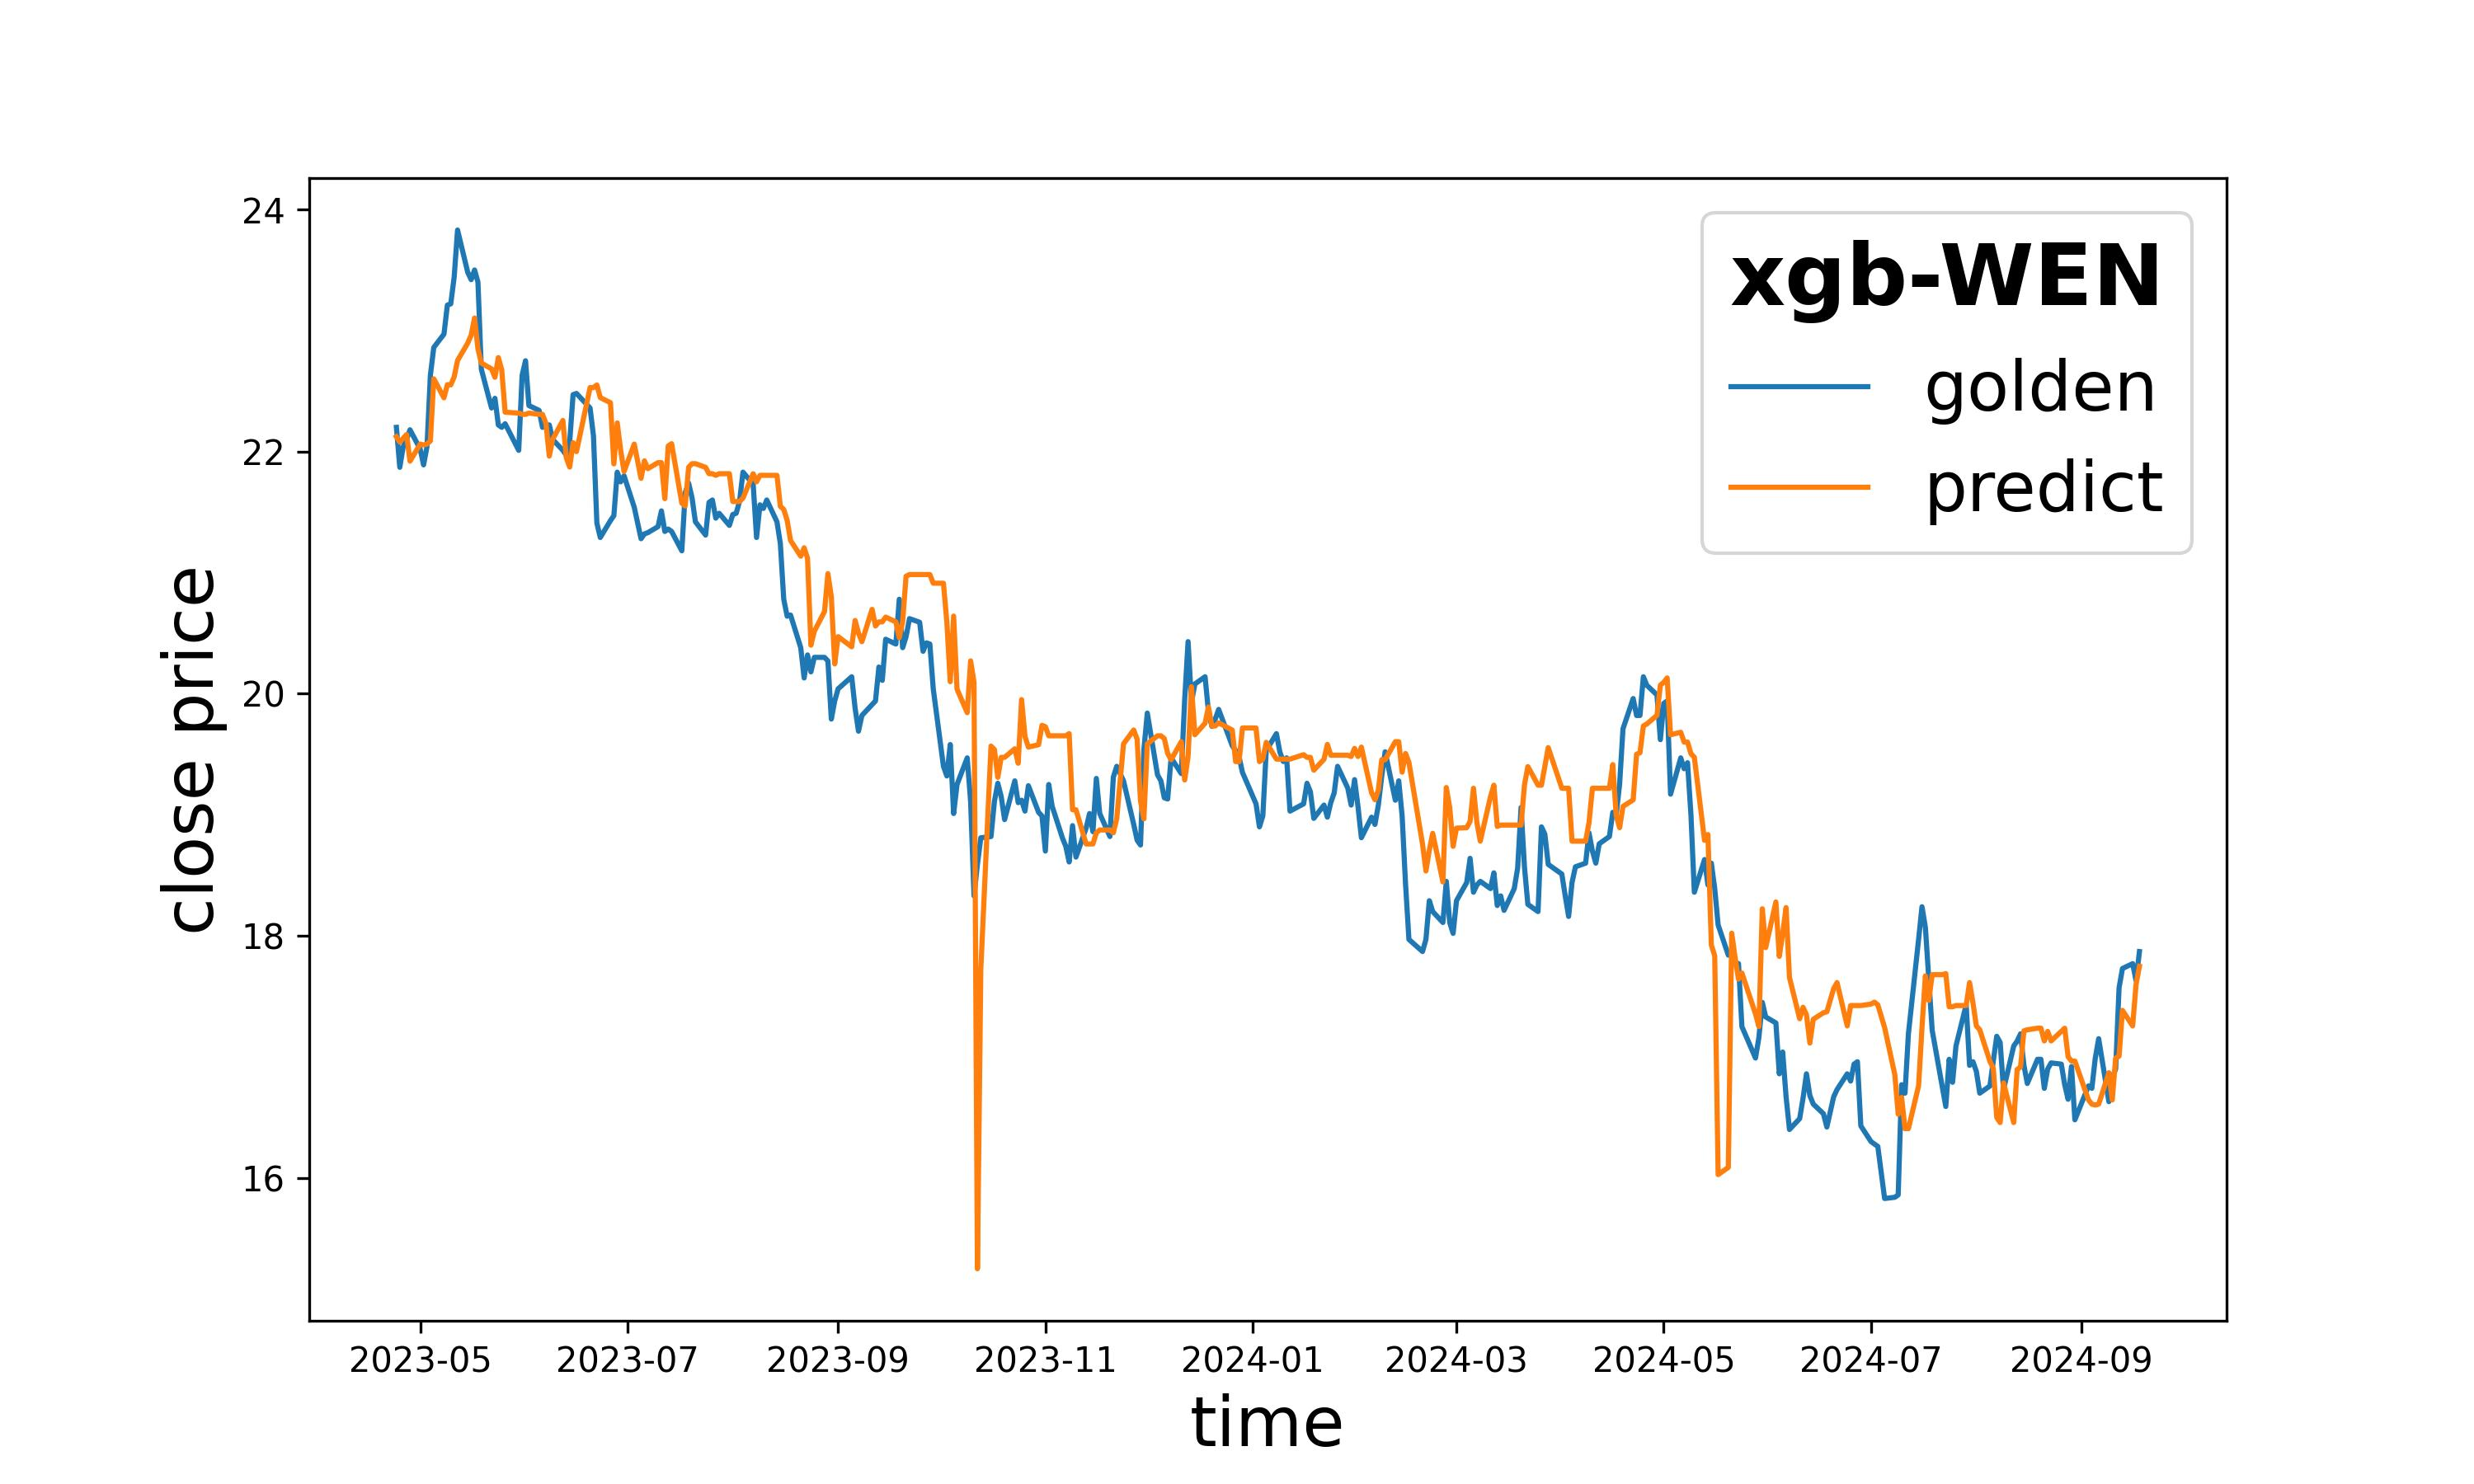
\includegraphics[width=\textwidth]{Result-Image/Result-Image3/05.WEN/xgb-WEN.jpg}
        \caption{XGBoost}
        \label{fig:image2}
    \end{subfigure}
    
    % 두 번째 행
    \vskip\baselineskip
    \begin{subfigure}[b]{0.49\textwidth}
        \centering
        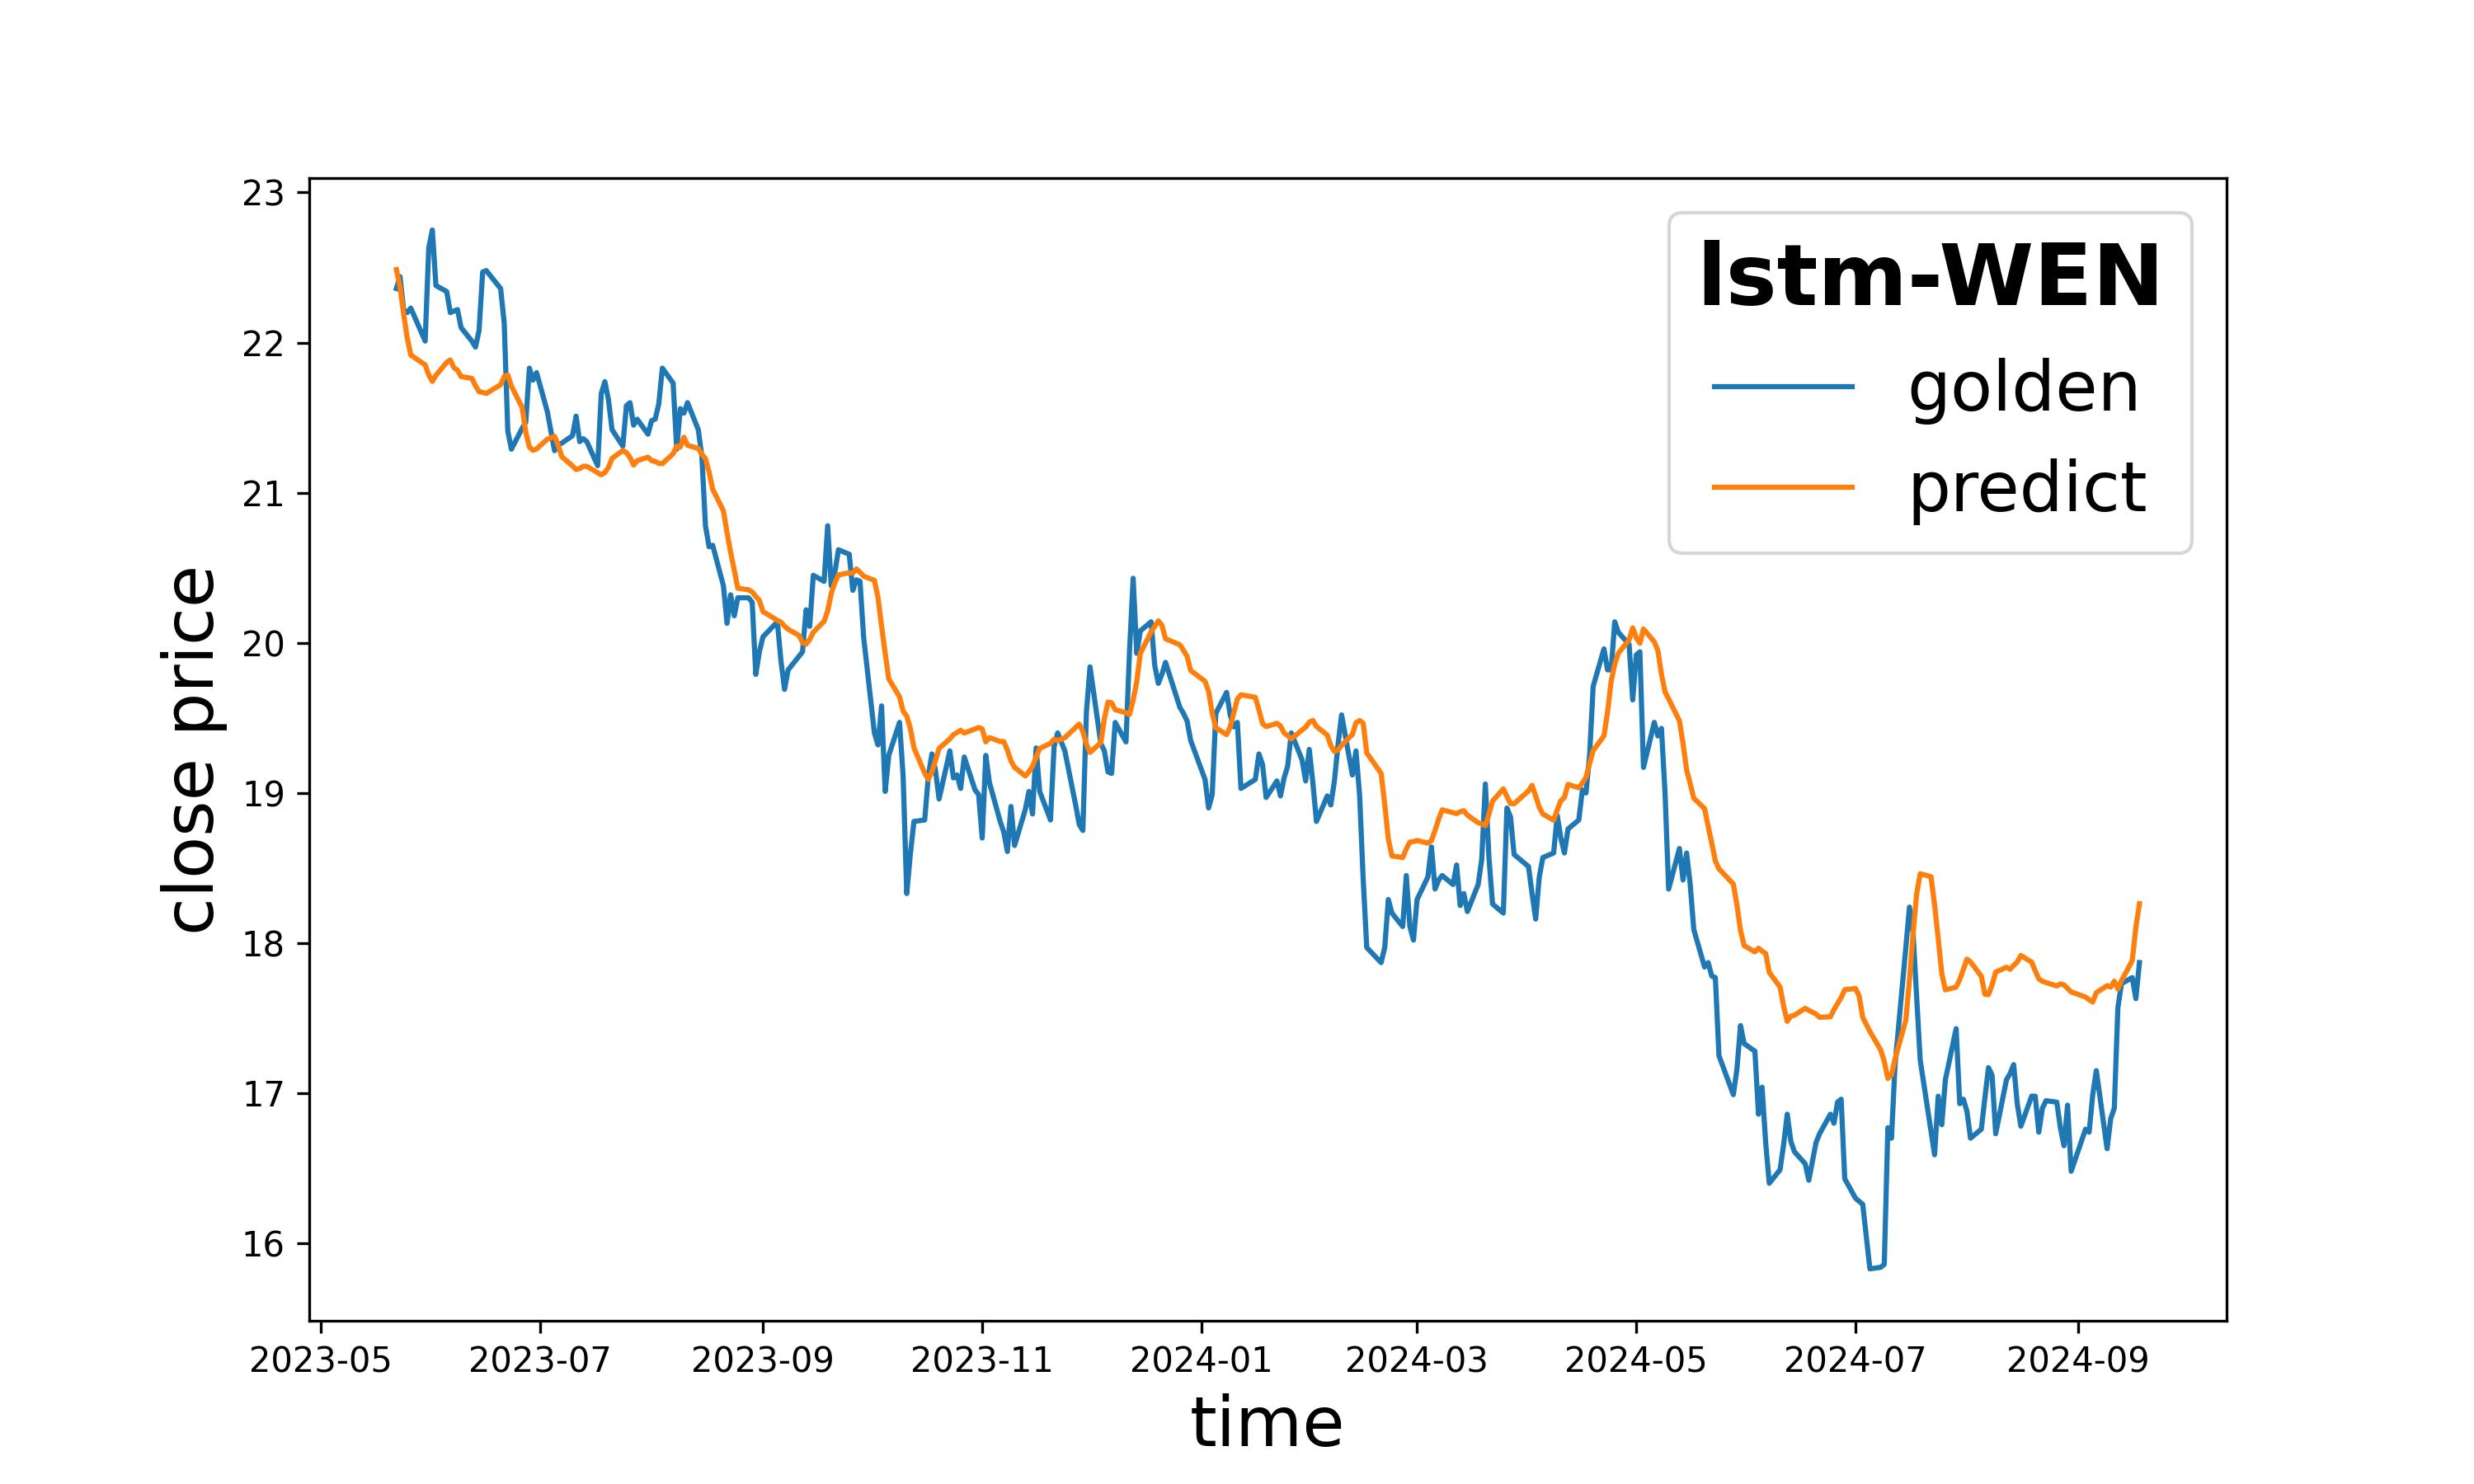
\includegraphics[width=\textwidth]{Result-Image/Result-Image3/05.WEN/lstm-WEN.jpg}
        \caption{LSTM}
        \label{fig:image3}
    \end{subfigure}
    \hfill
    \begin{subfigure}[b]{0.49\textwidth}
        \centering
        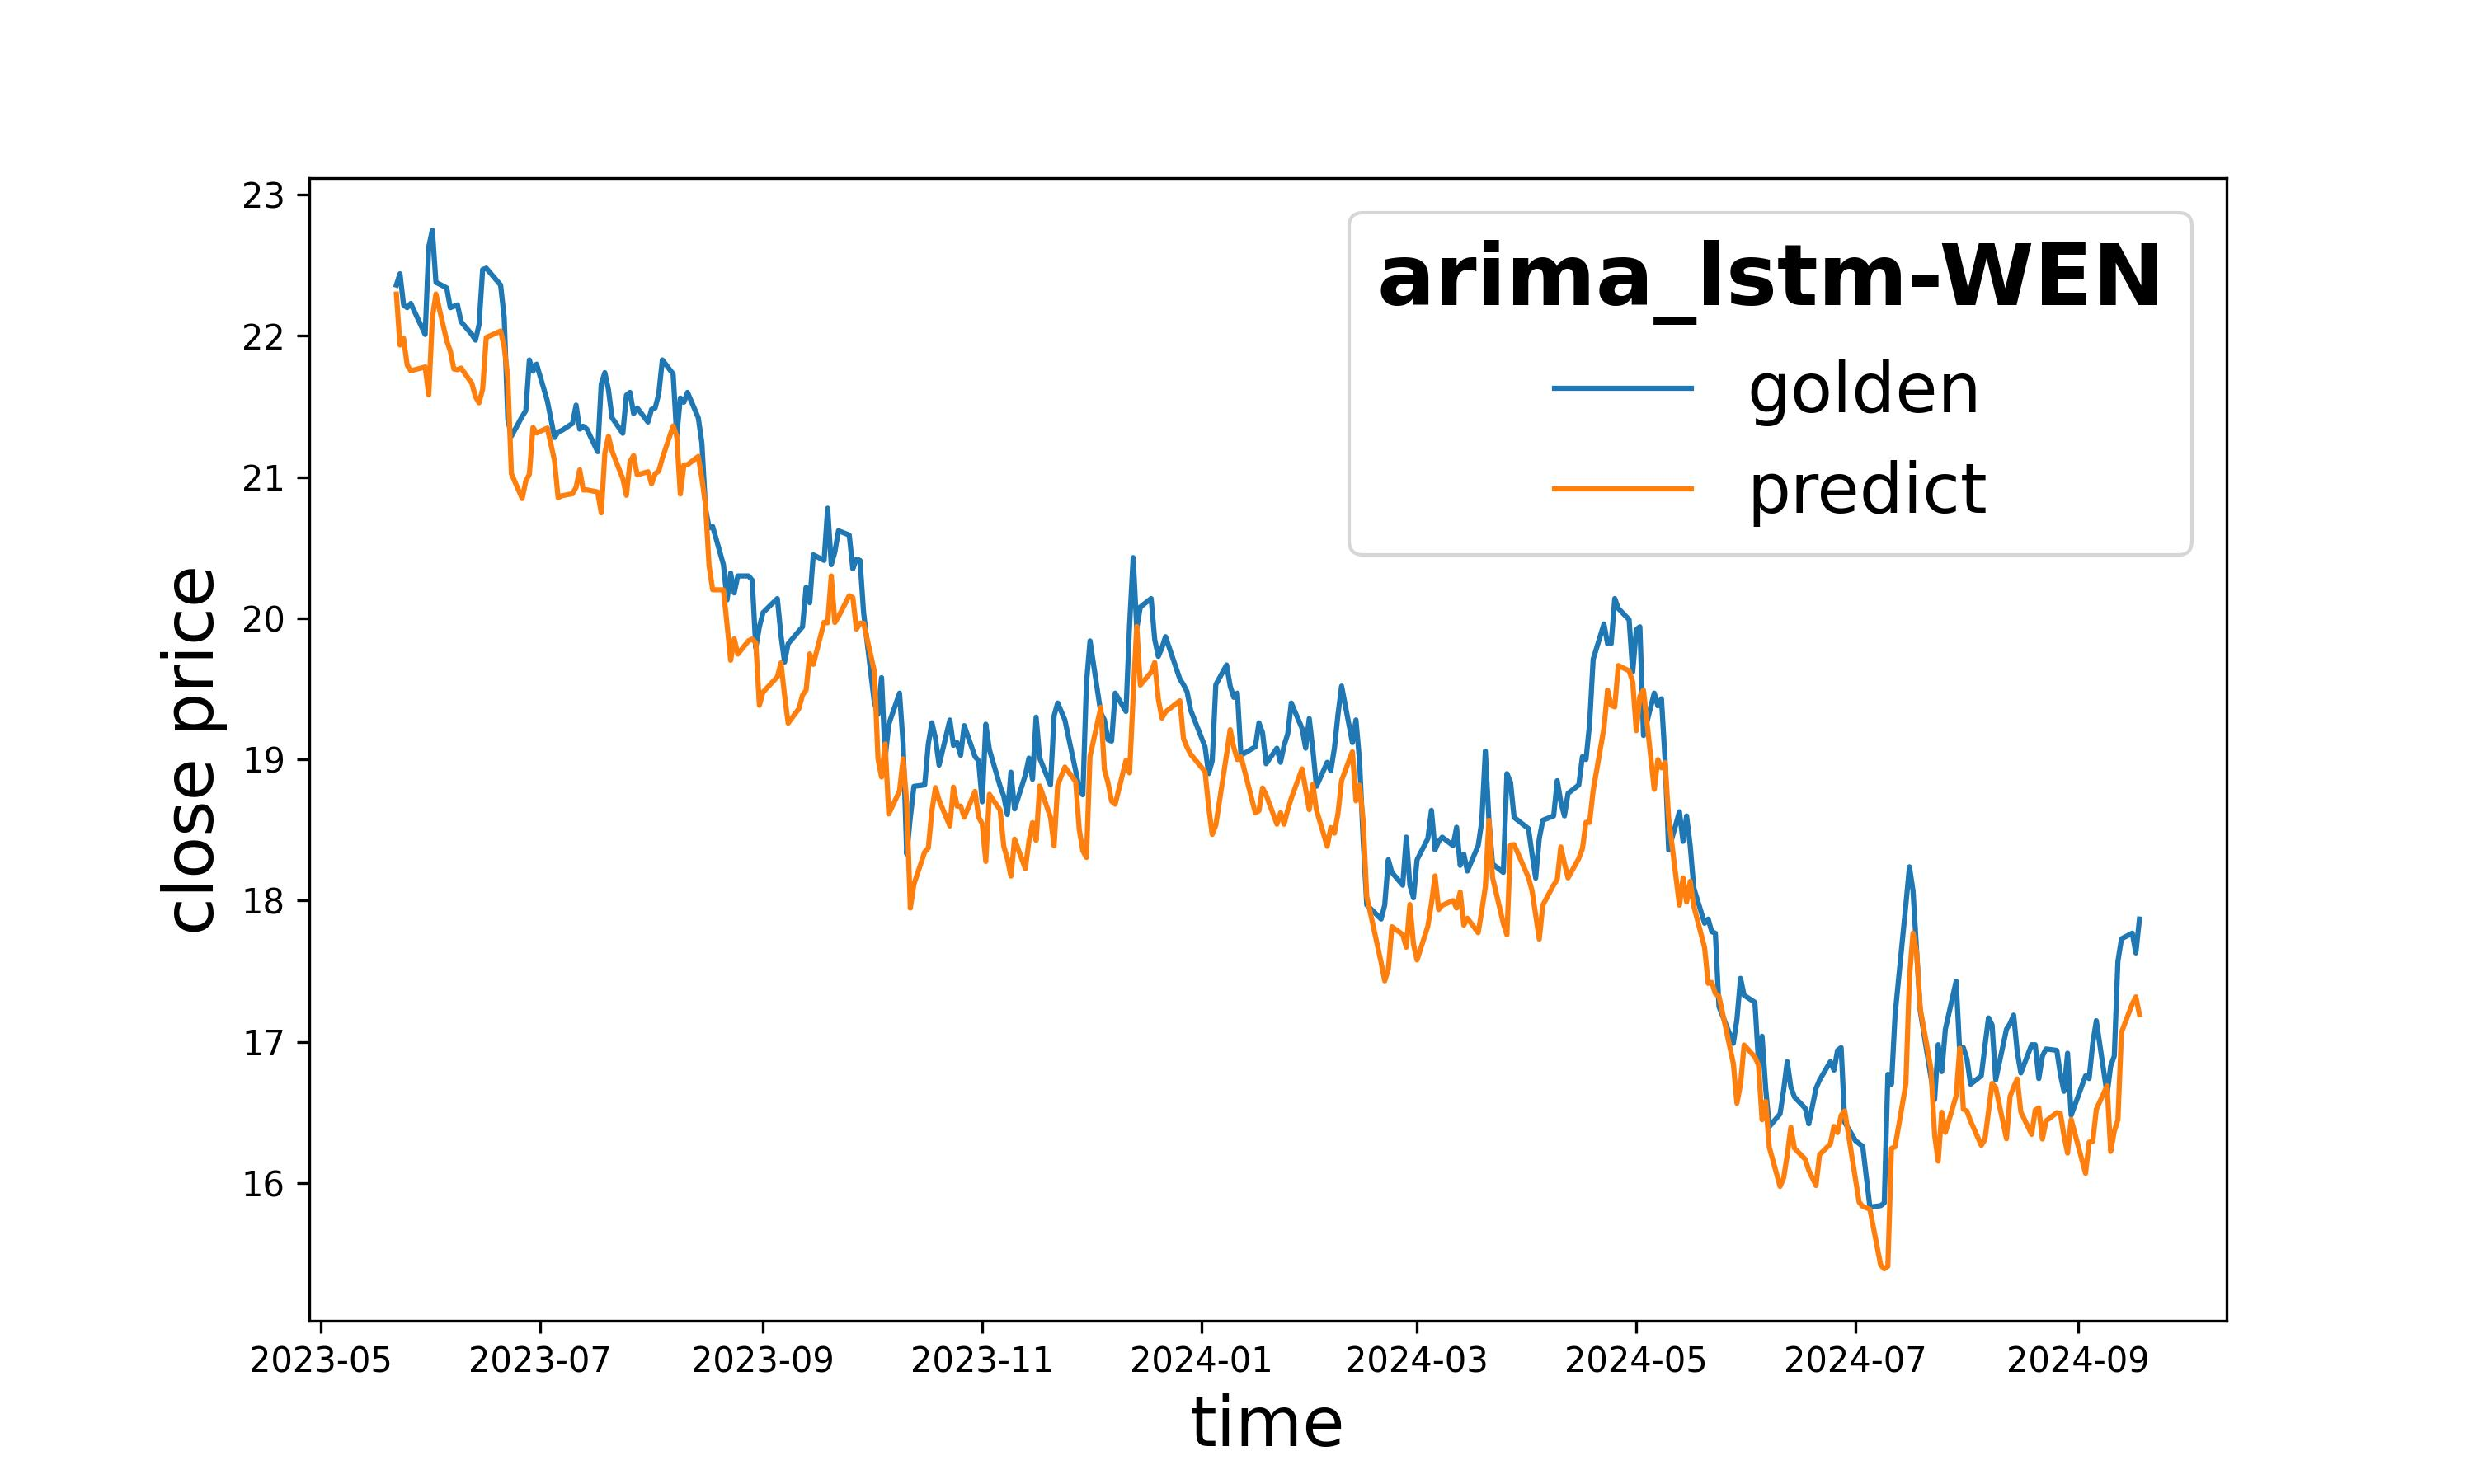
\includegraphics[width=\textwidth]{Result-Image/Result-Image3/05.WEN/arima_lstm-WEN.jpg}
        \caption{ARIMA-LSTM}
        \label{fig:image4}
    \end{subfigure}
    
    \caption{WEN}
    \label{fig:2x2grid}
\end{figure}


%\subsection{DNUT}
\begin{figure}[ht]
    \centering
    \begin{subfigure}[b]{0.49\textwidth}
        \centering
        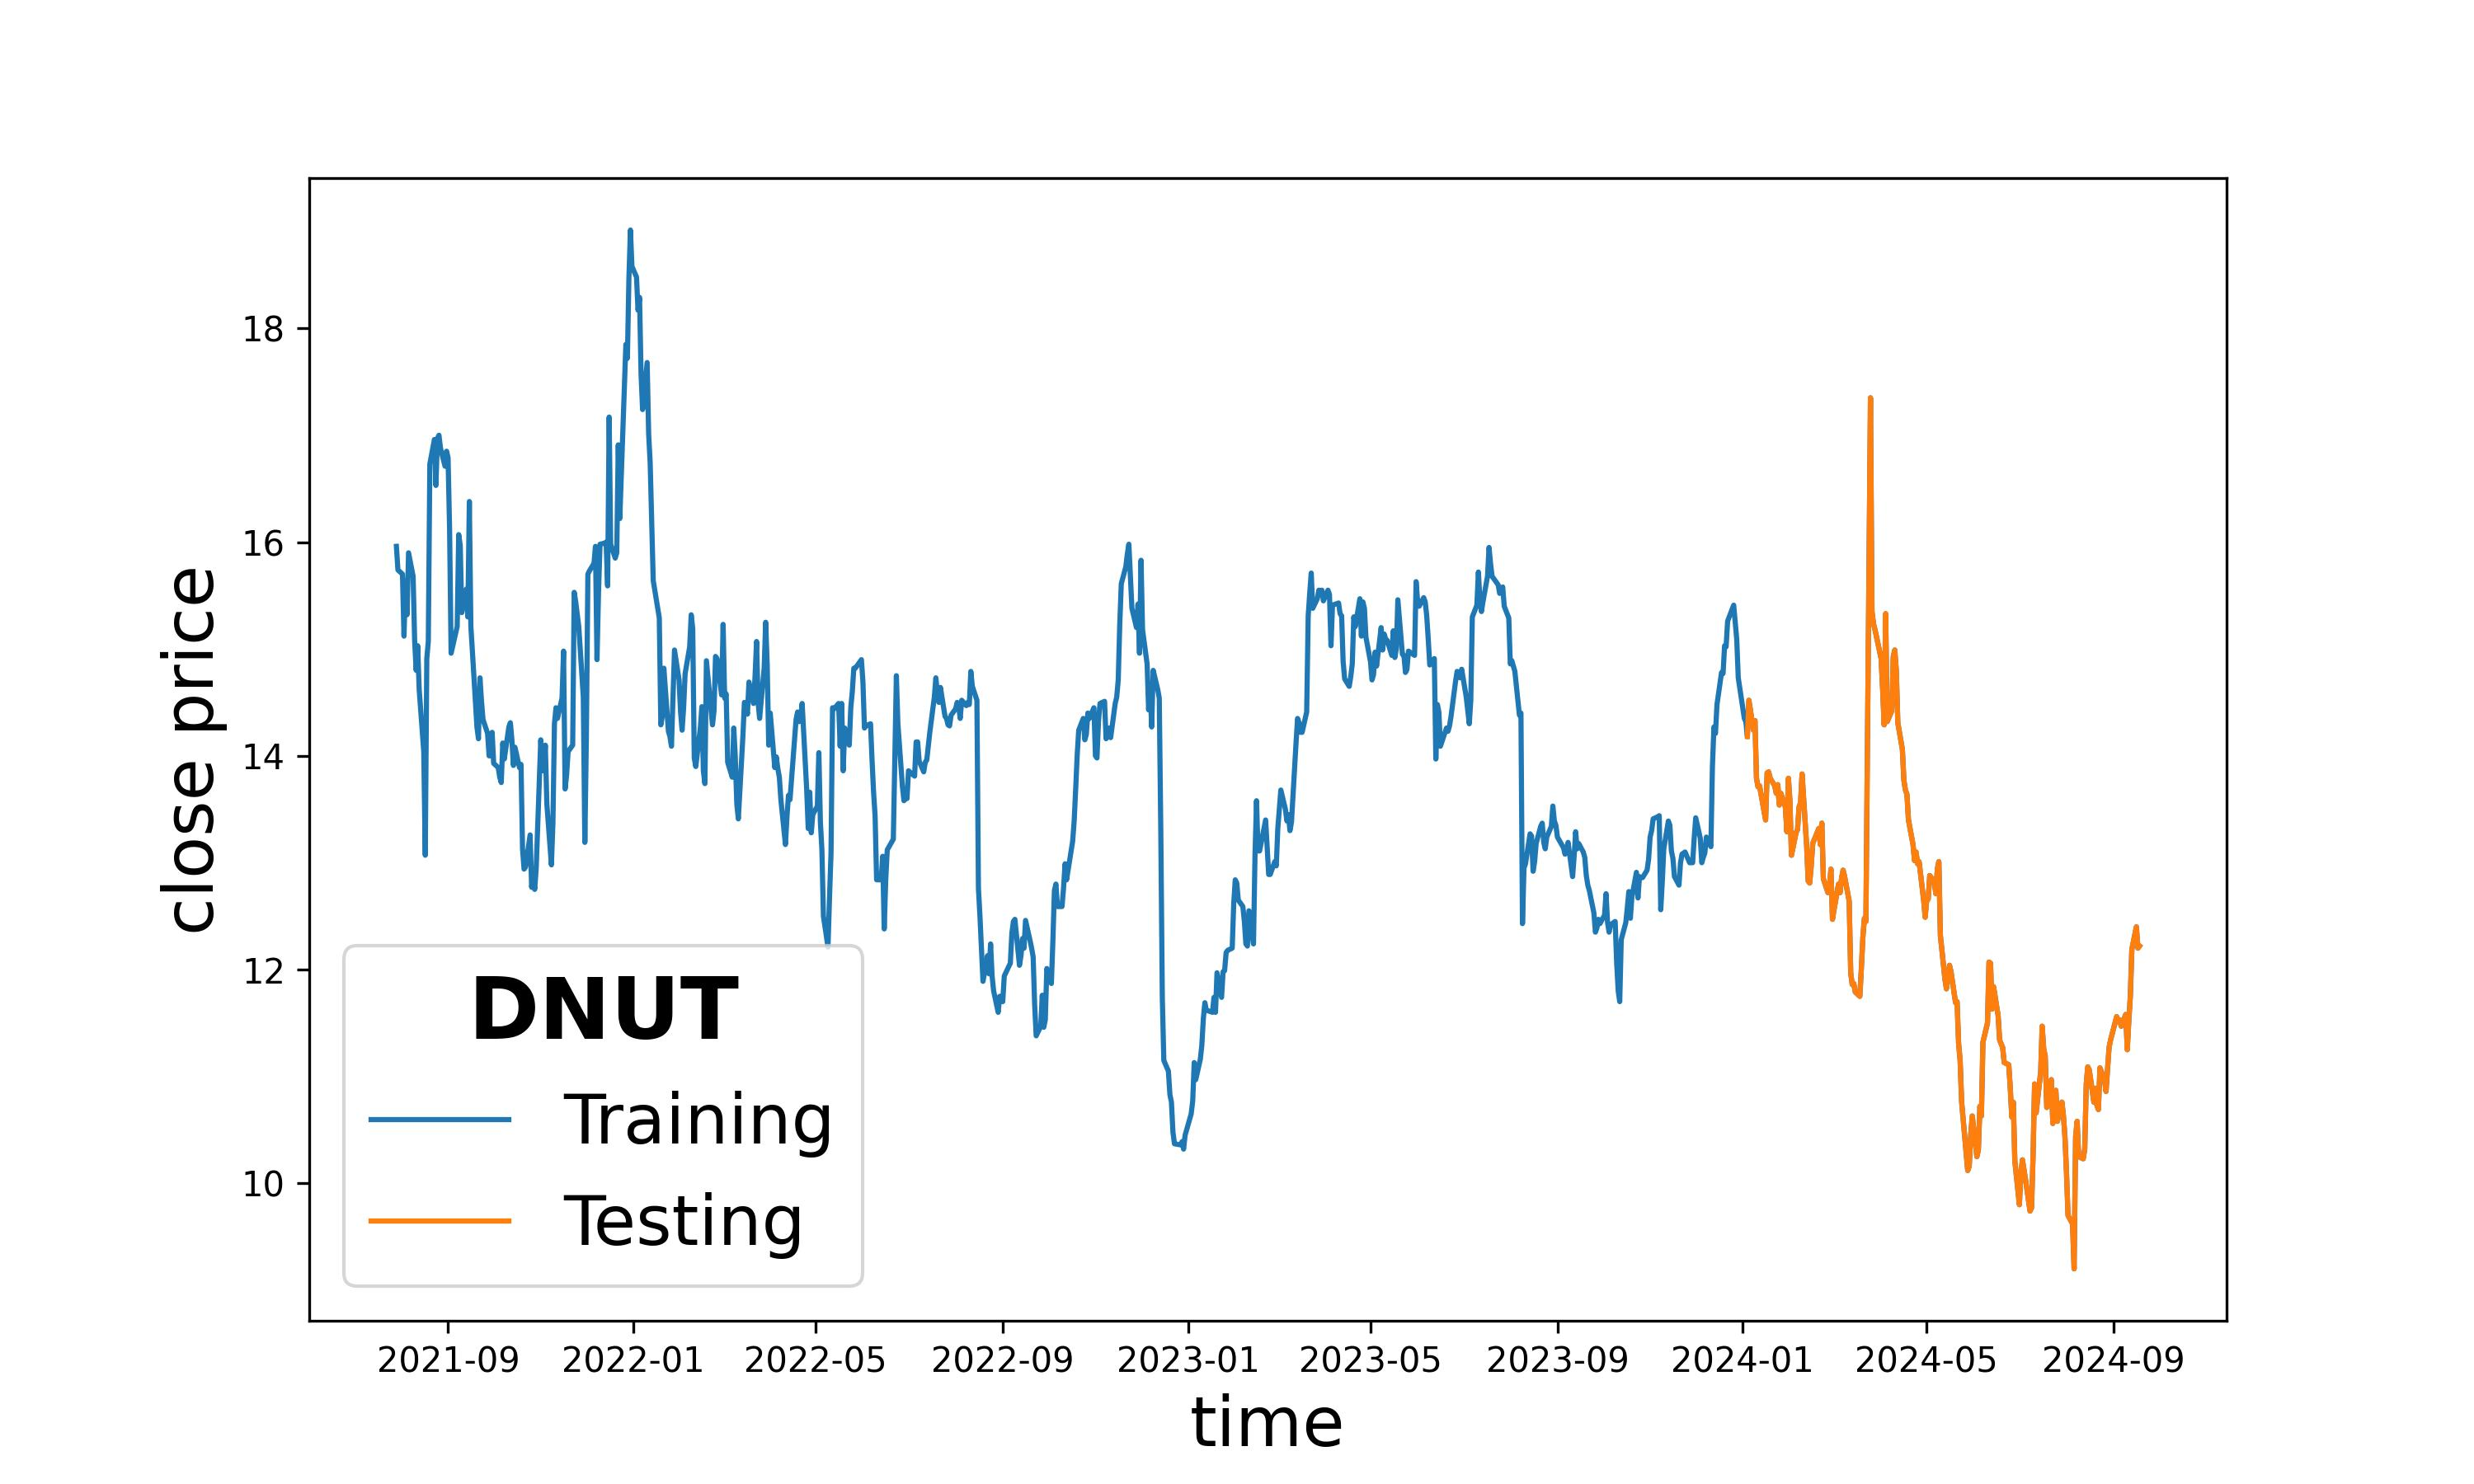
\includegraphics[width=\textwidth]{Result-Image/Result-Image3/06.DNUT/DNUT.jpg}
        \caption{Training/Testing}
        \label{fig:image1}
    \end{subfigure}
    
    % 첫 번째 행
    \begin{subfigure}[b]{0.49\textwidth}
        \centering
        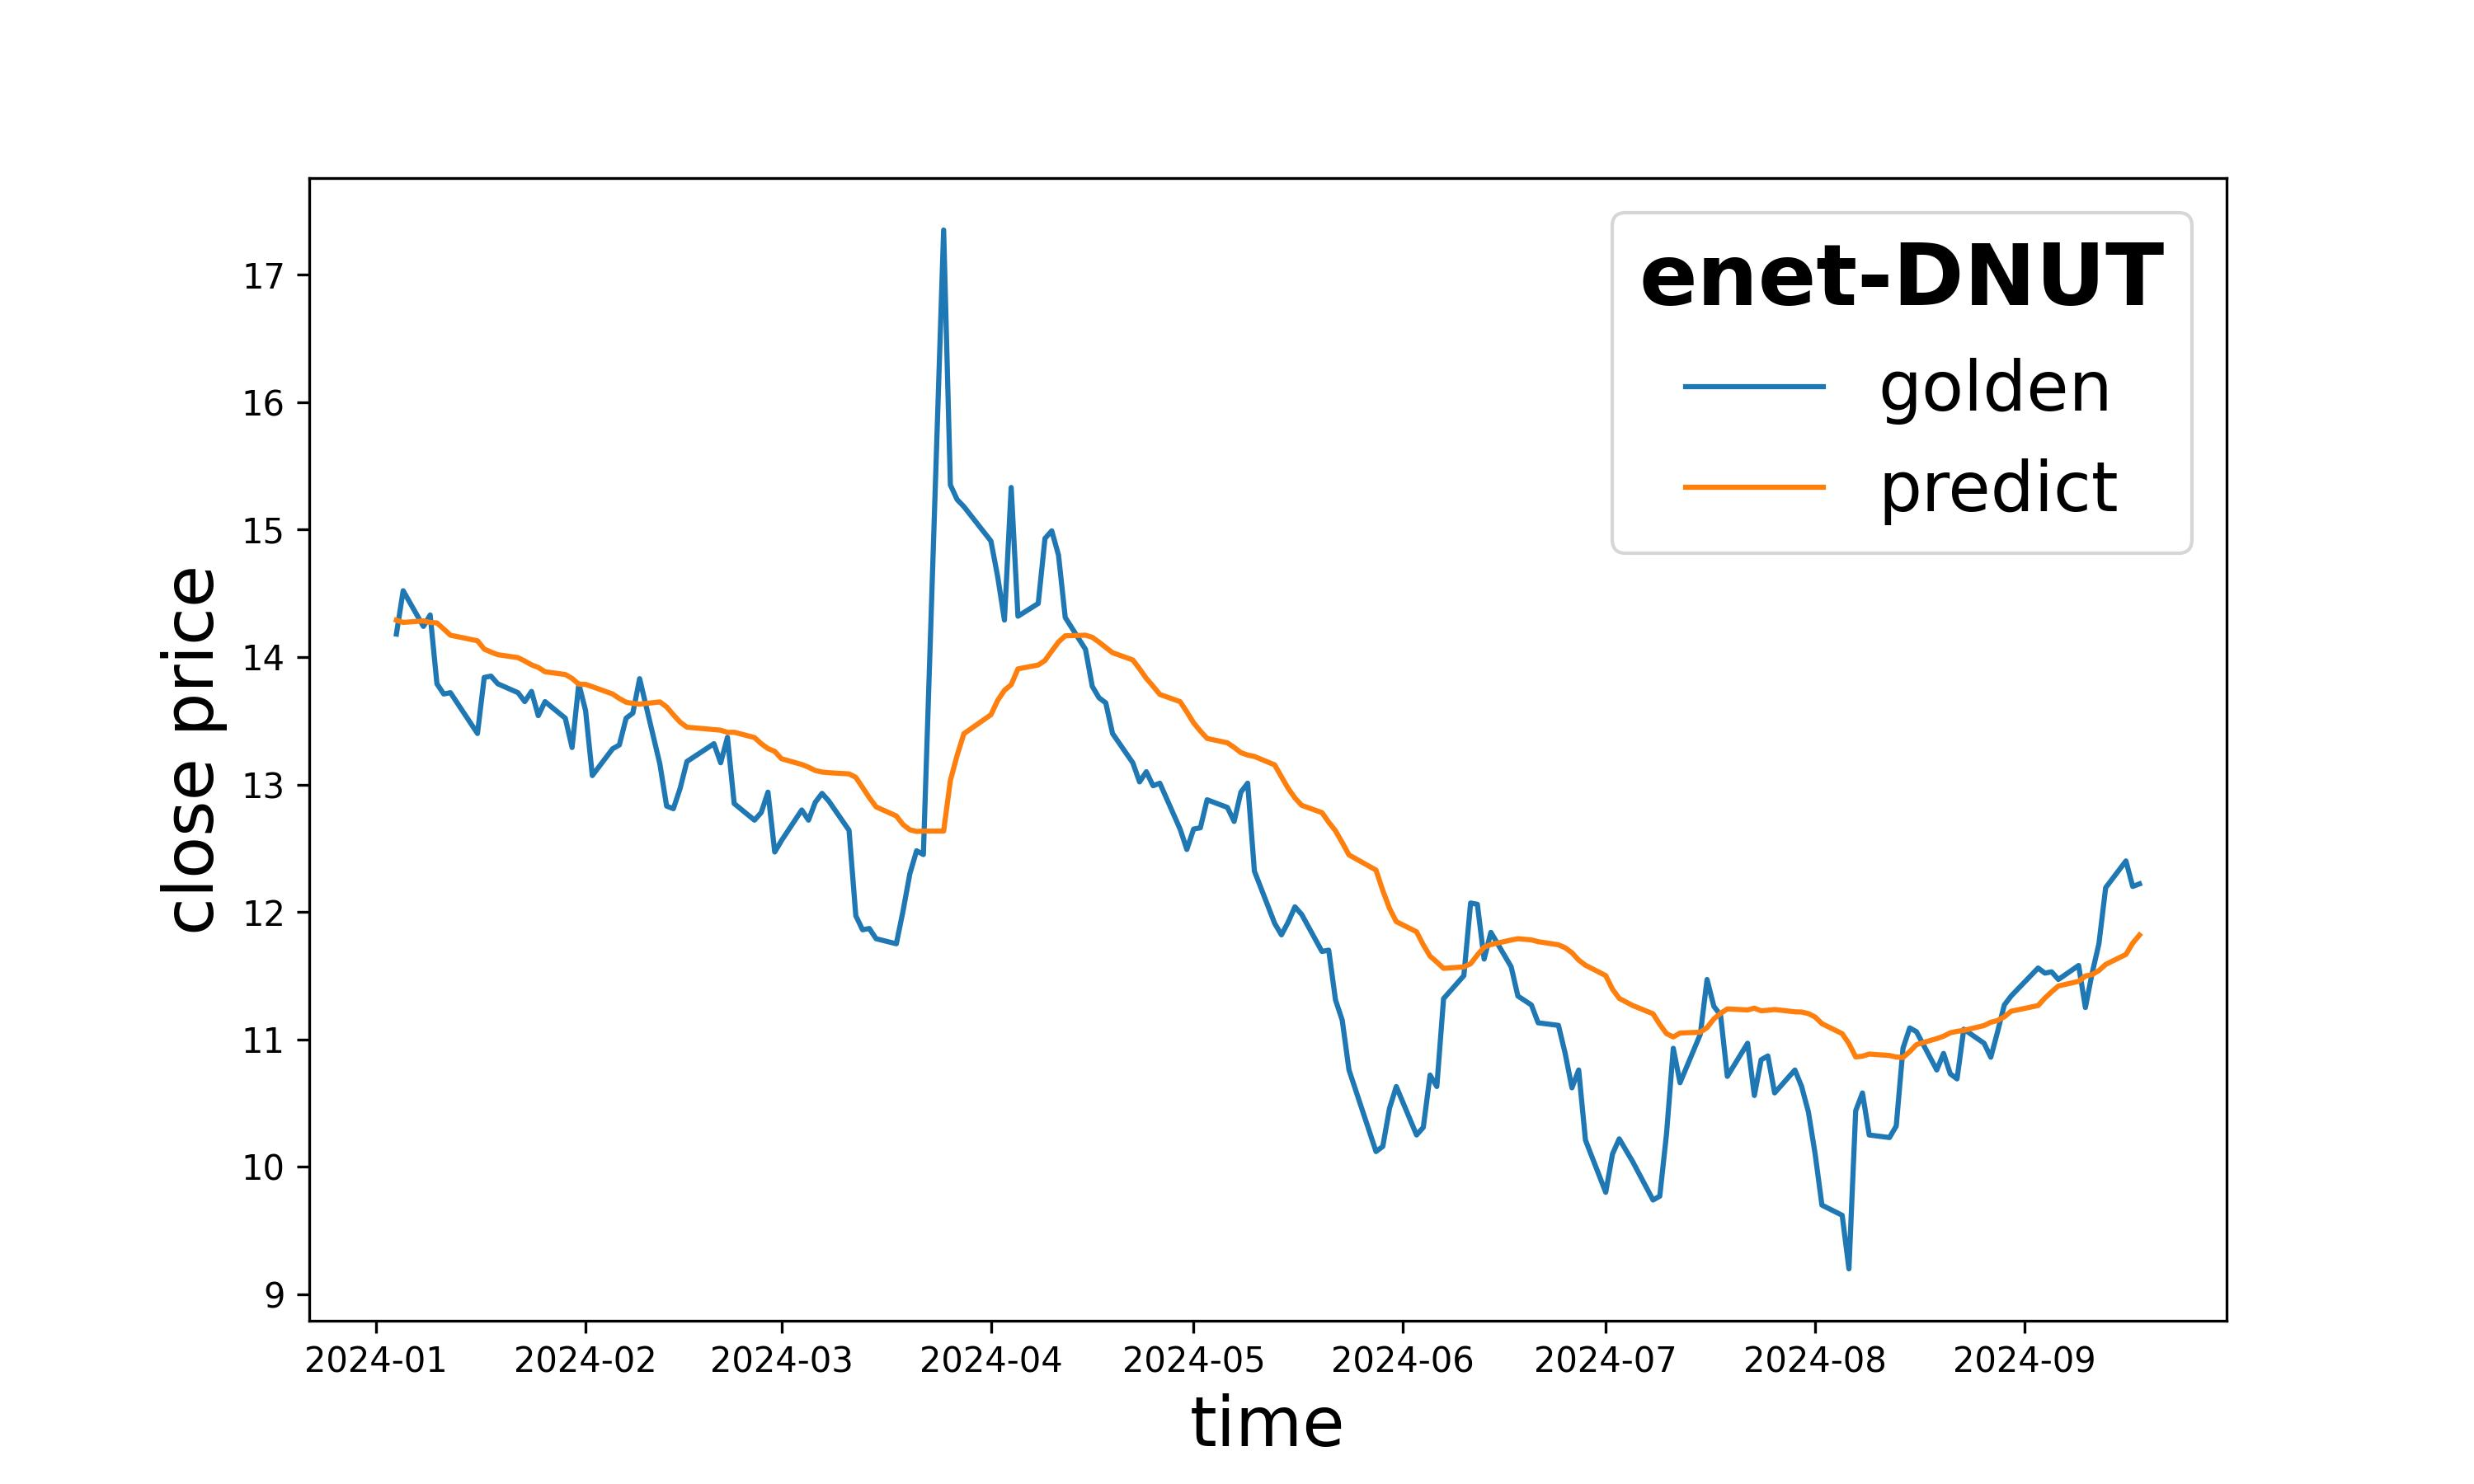
\includegraphics[width=\textwidth]{Result-Image/Result-Image3/06.DNUT/enet-DNUT.jpg}
        \caption{Enet}
        \label{fig:image1}
    \end{subfigure}
    \hfill
    \begin{subfigure}[b]{0.49\textwidth}
        \centering
        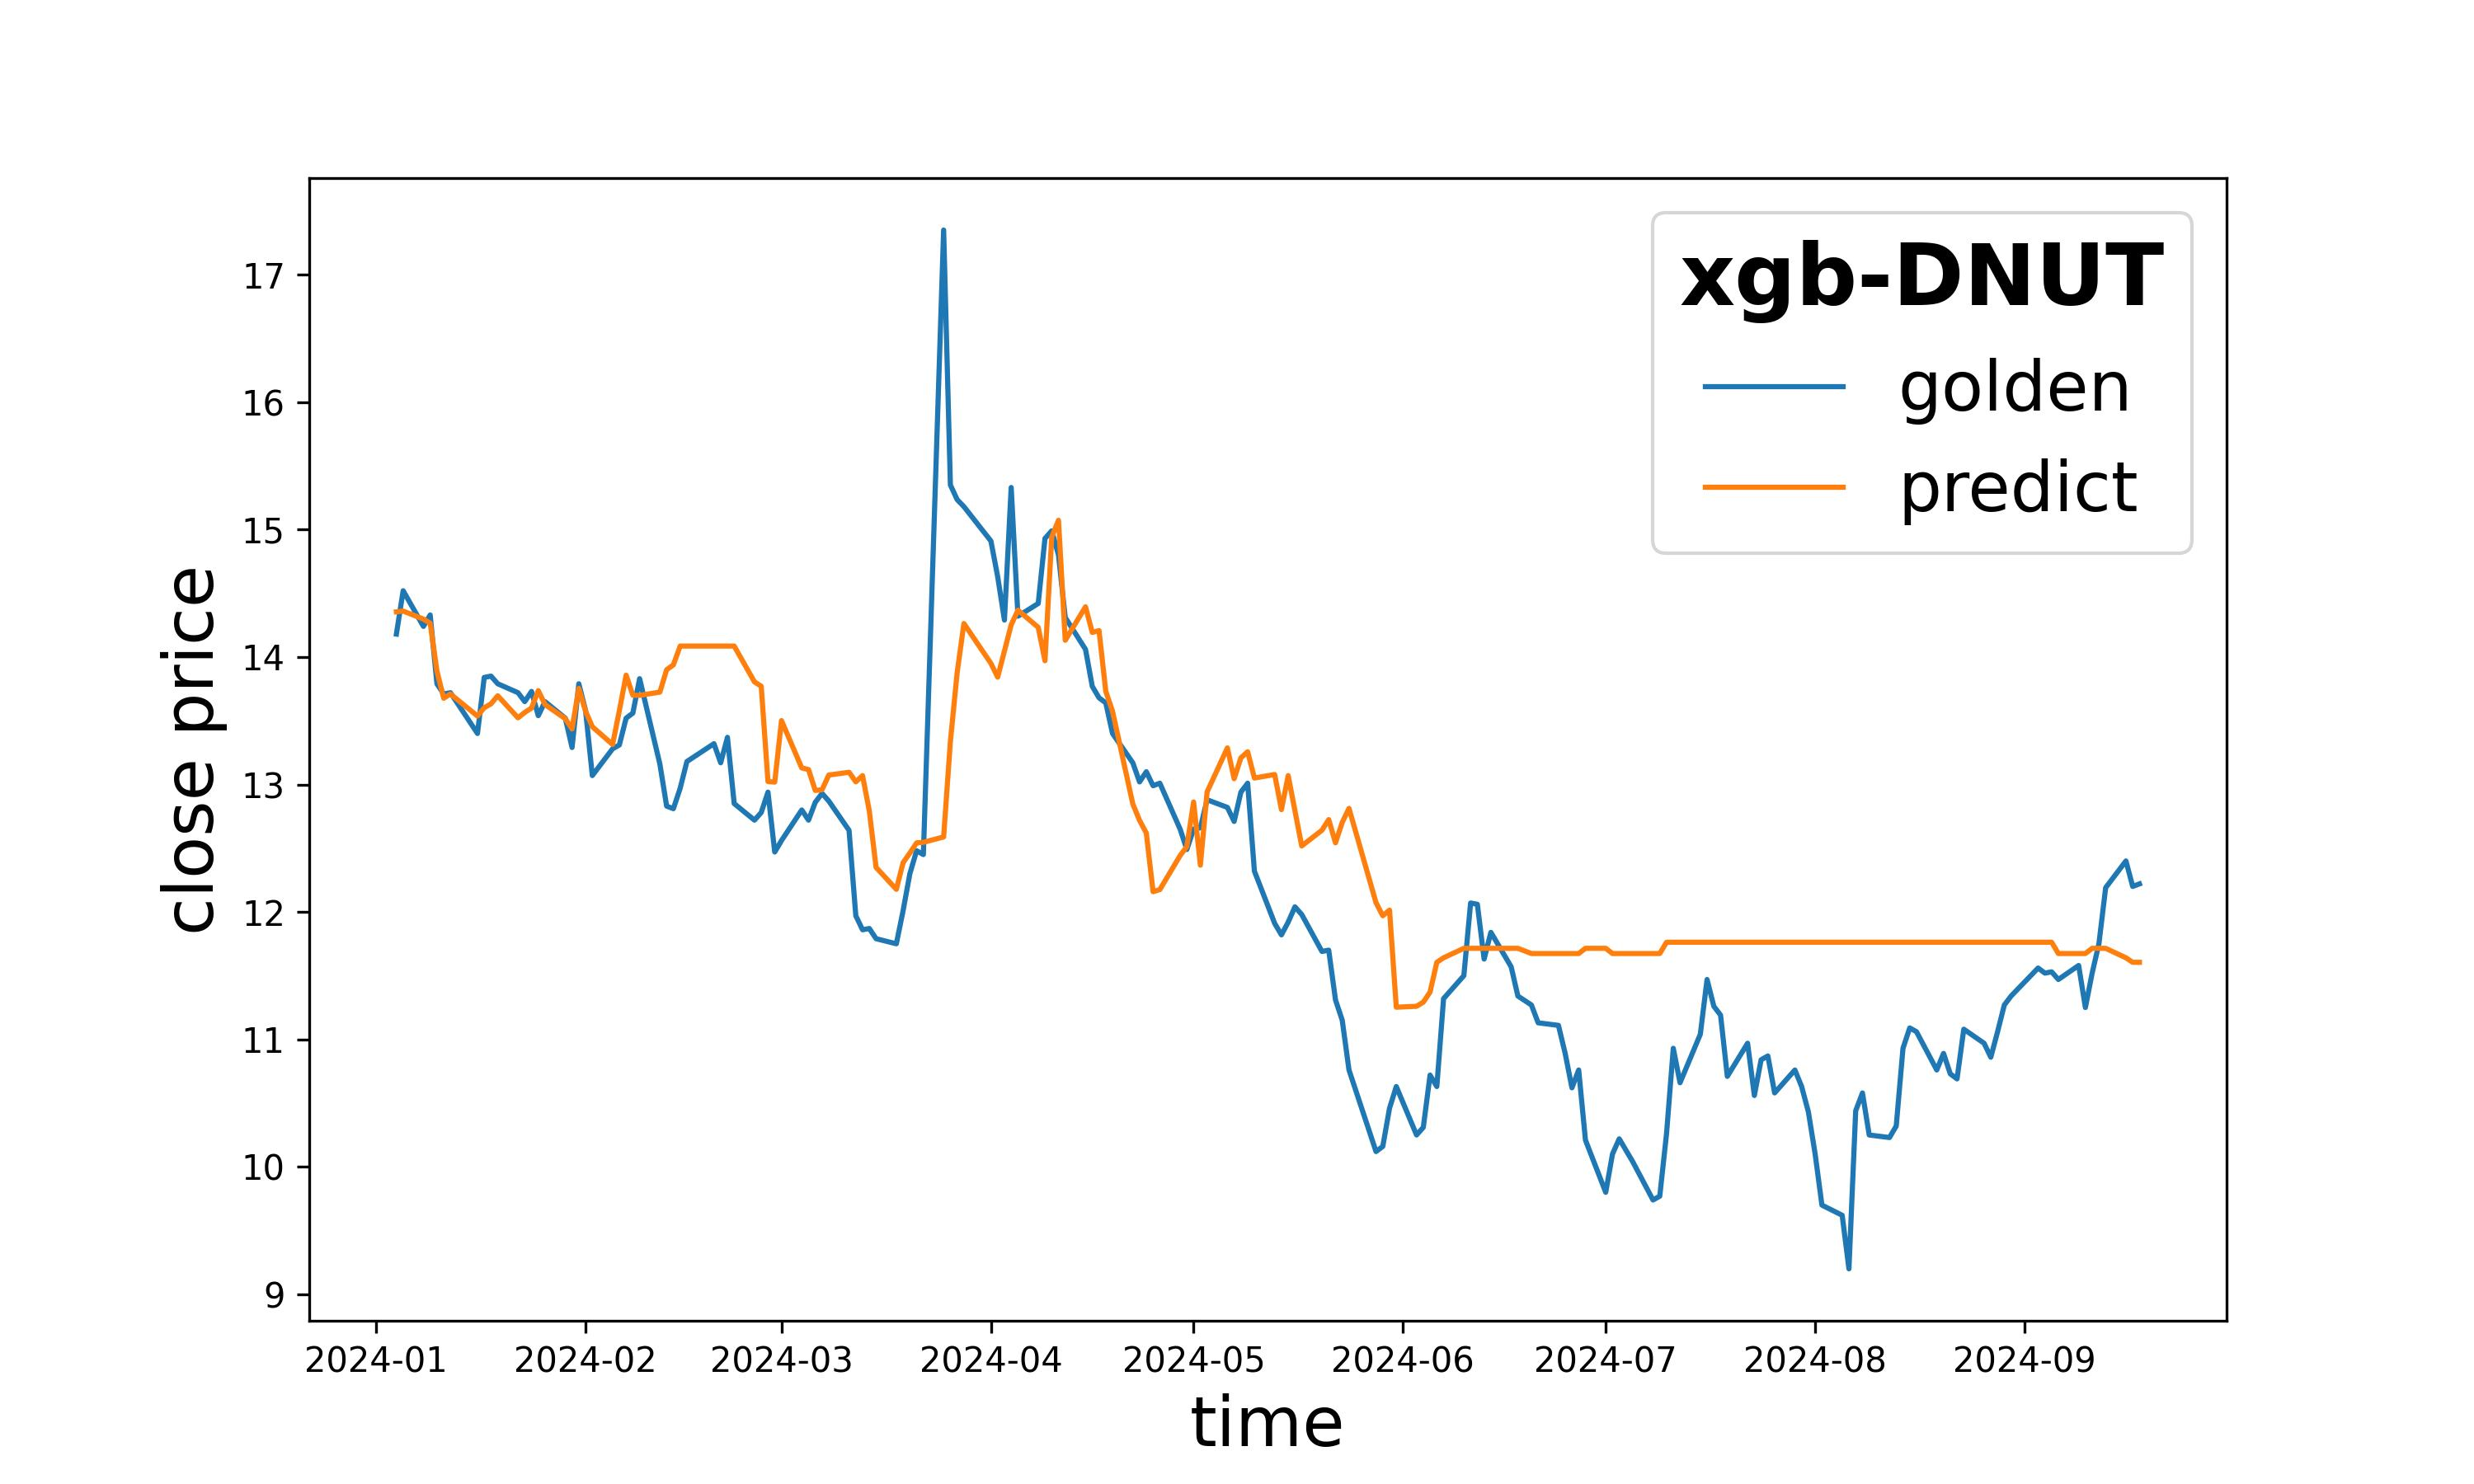
\includegraphics[width=\textwidth]{Result-Image/Result-Image3/06.DNUT/xgb-DNUT.jpg}
        \caption{XGBoost}
        \label{fig:image2}
    \end{subfigure}
    
    % 두 번째 행
    \vskip\baselineskip
    \begin{subfigure}[b]{0.49\textwidth}
        \centering
        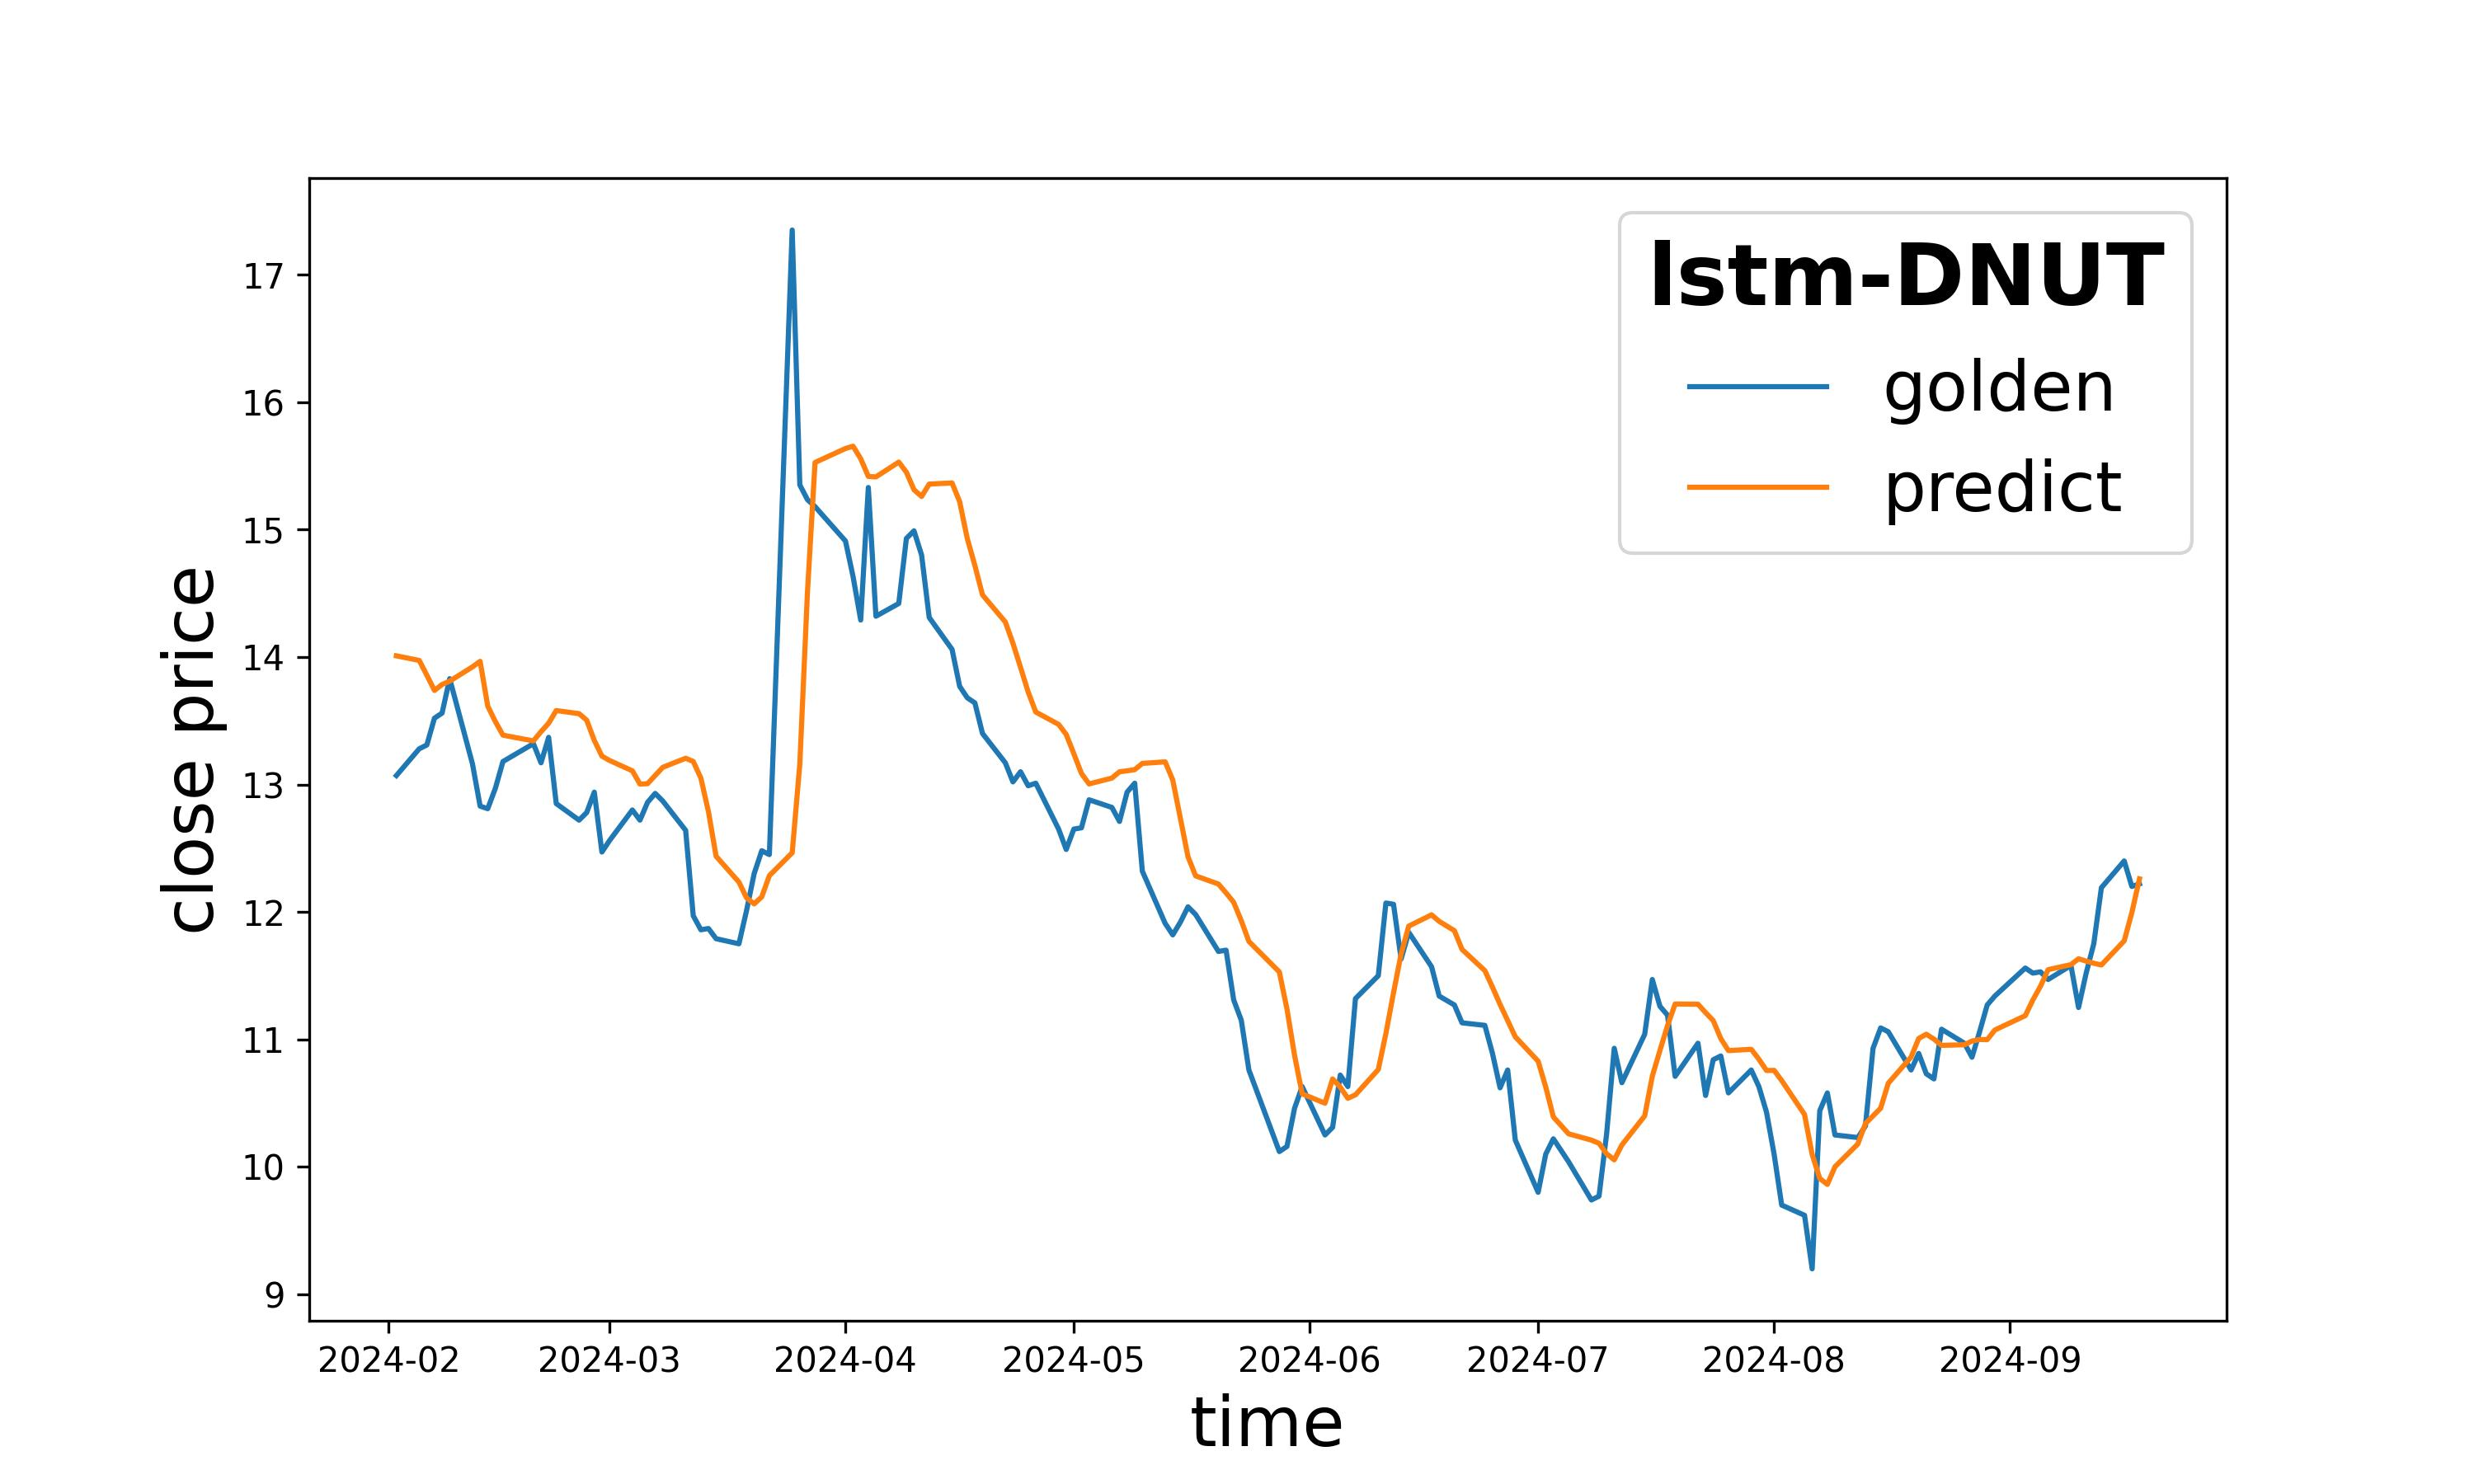
\includegraphics[width=\textwidth]{Result-Image/Result-Image3/06.DNUT/lstm-DNUT.jpg}
        \caption{LSTM}
        \label{fig:image3}
    \end{subfigure}
    \hfill
    \begin{subfigure}[b]{0.49\textwidth}
        \centering
        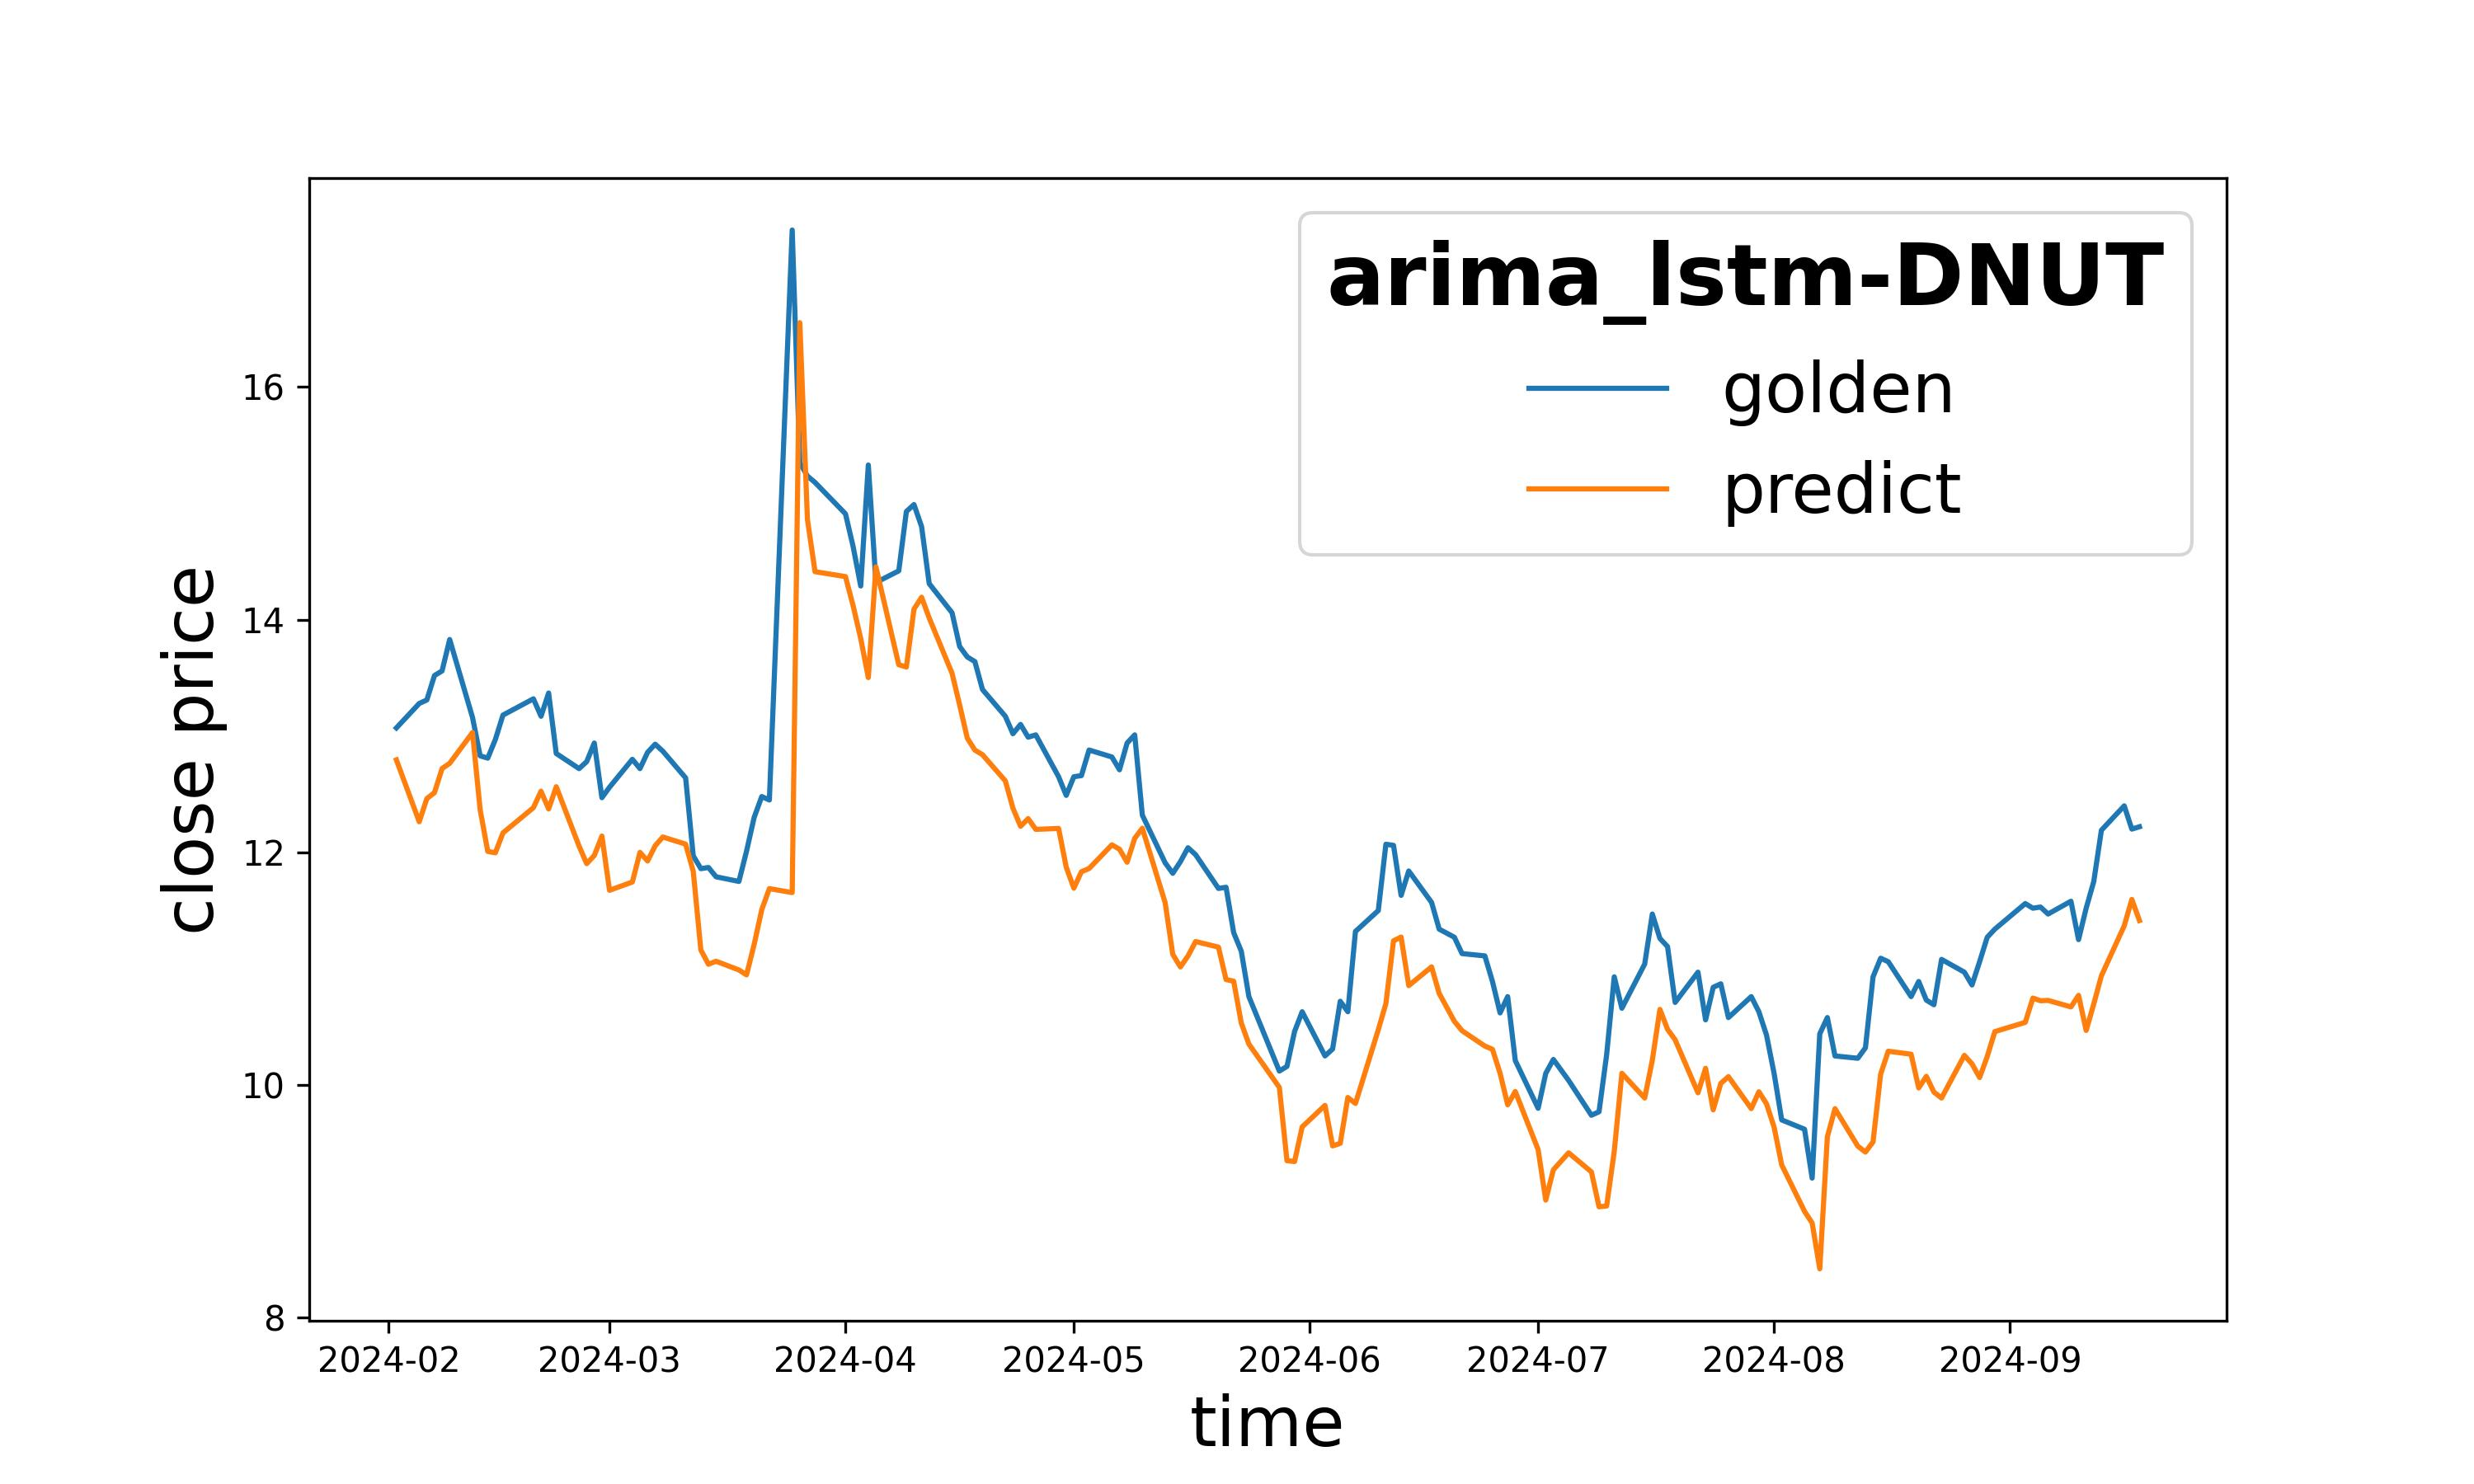
\includegraphics[width=\textwidth]{Result-Image/Result-Image3/06.DNUT/arima_lstm-DNUT.jpg}
        \caption{ARIMA-LSTM}
        \label{fig:image4}
    \end{subfigure}
    
    \caption{DNUT}
    \label{fig:2x2grid}
\end{figure}

%\subsection{LKNCY}
\begin{figure}[ht]
    \centering
    \begin{subfigure}[b]{0.49\textwidth}
        \centering
        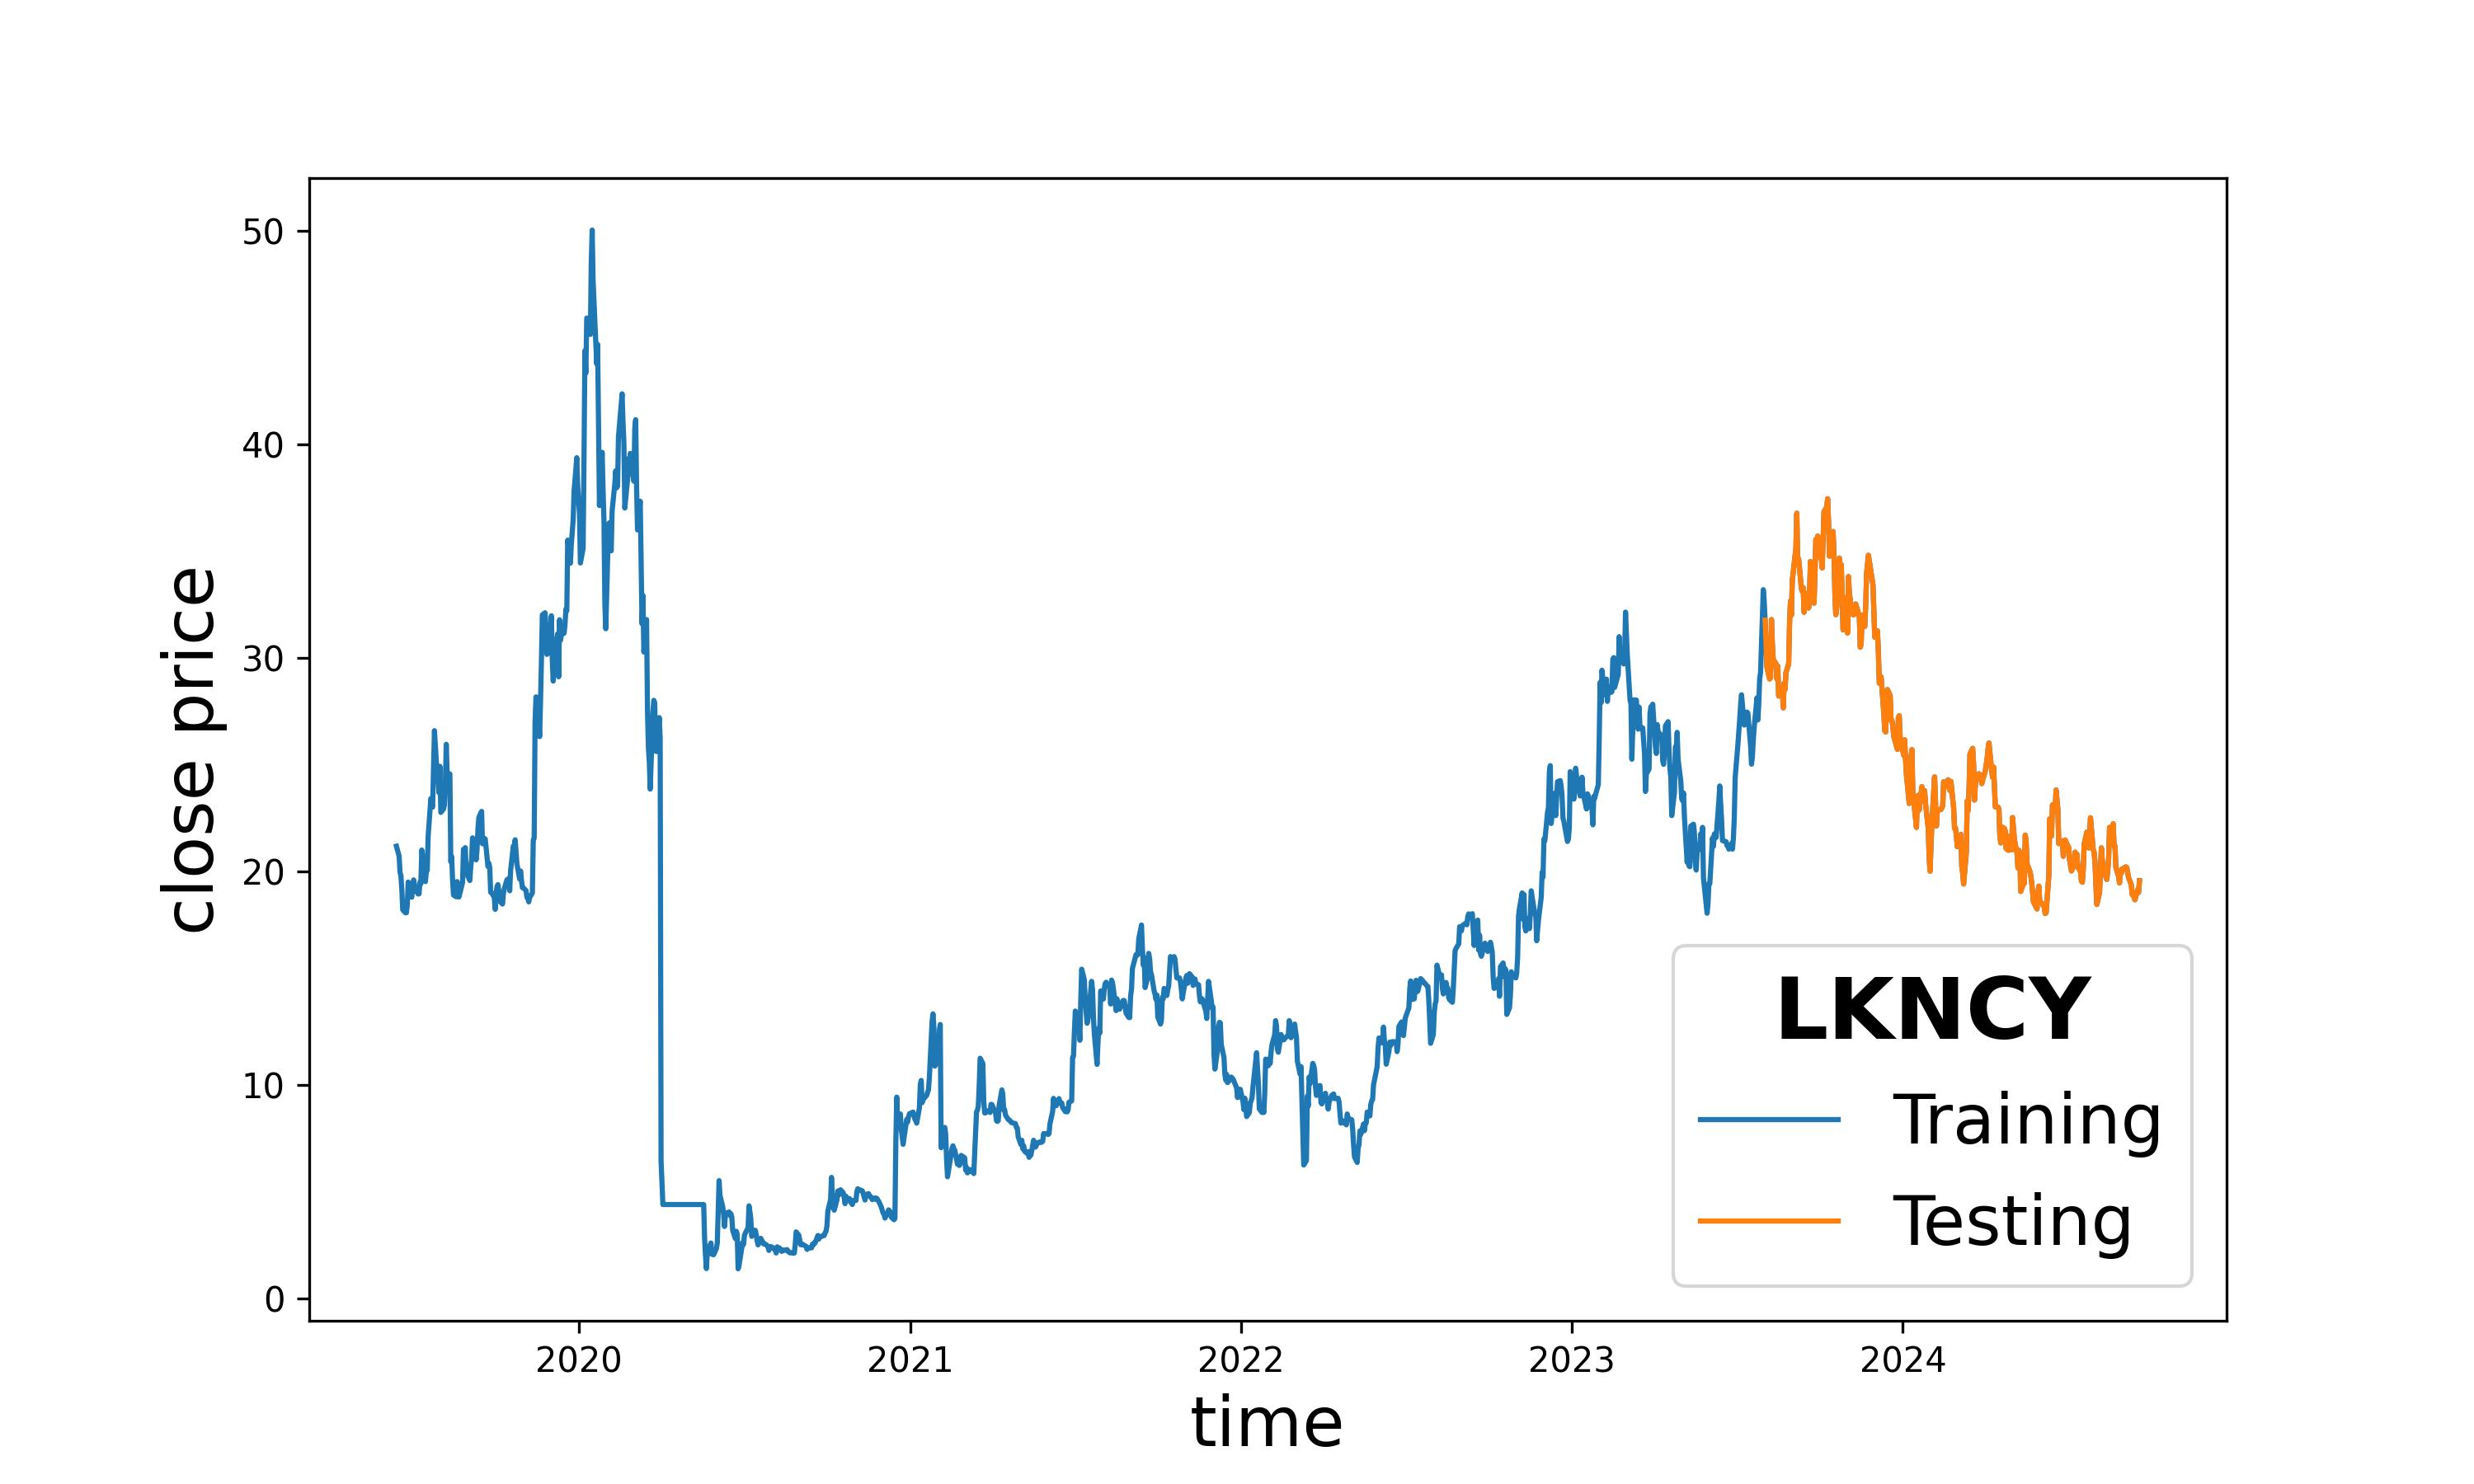
\includegraphics[width=\textwidth]{Result-Image/Result-Image3/07.LKNCY/LKNCY.jpg}
        \caption{Training/Testing}
        \label{fig:image1}
    \end{subfigure}
    
    % 첫 번째 행
    \begin{subfigure}[b]{0.49\textwidth}
        \centering
        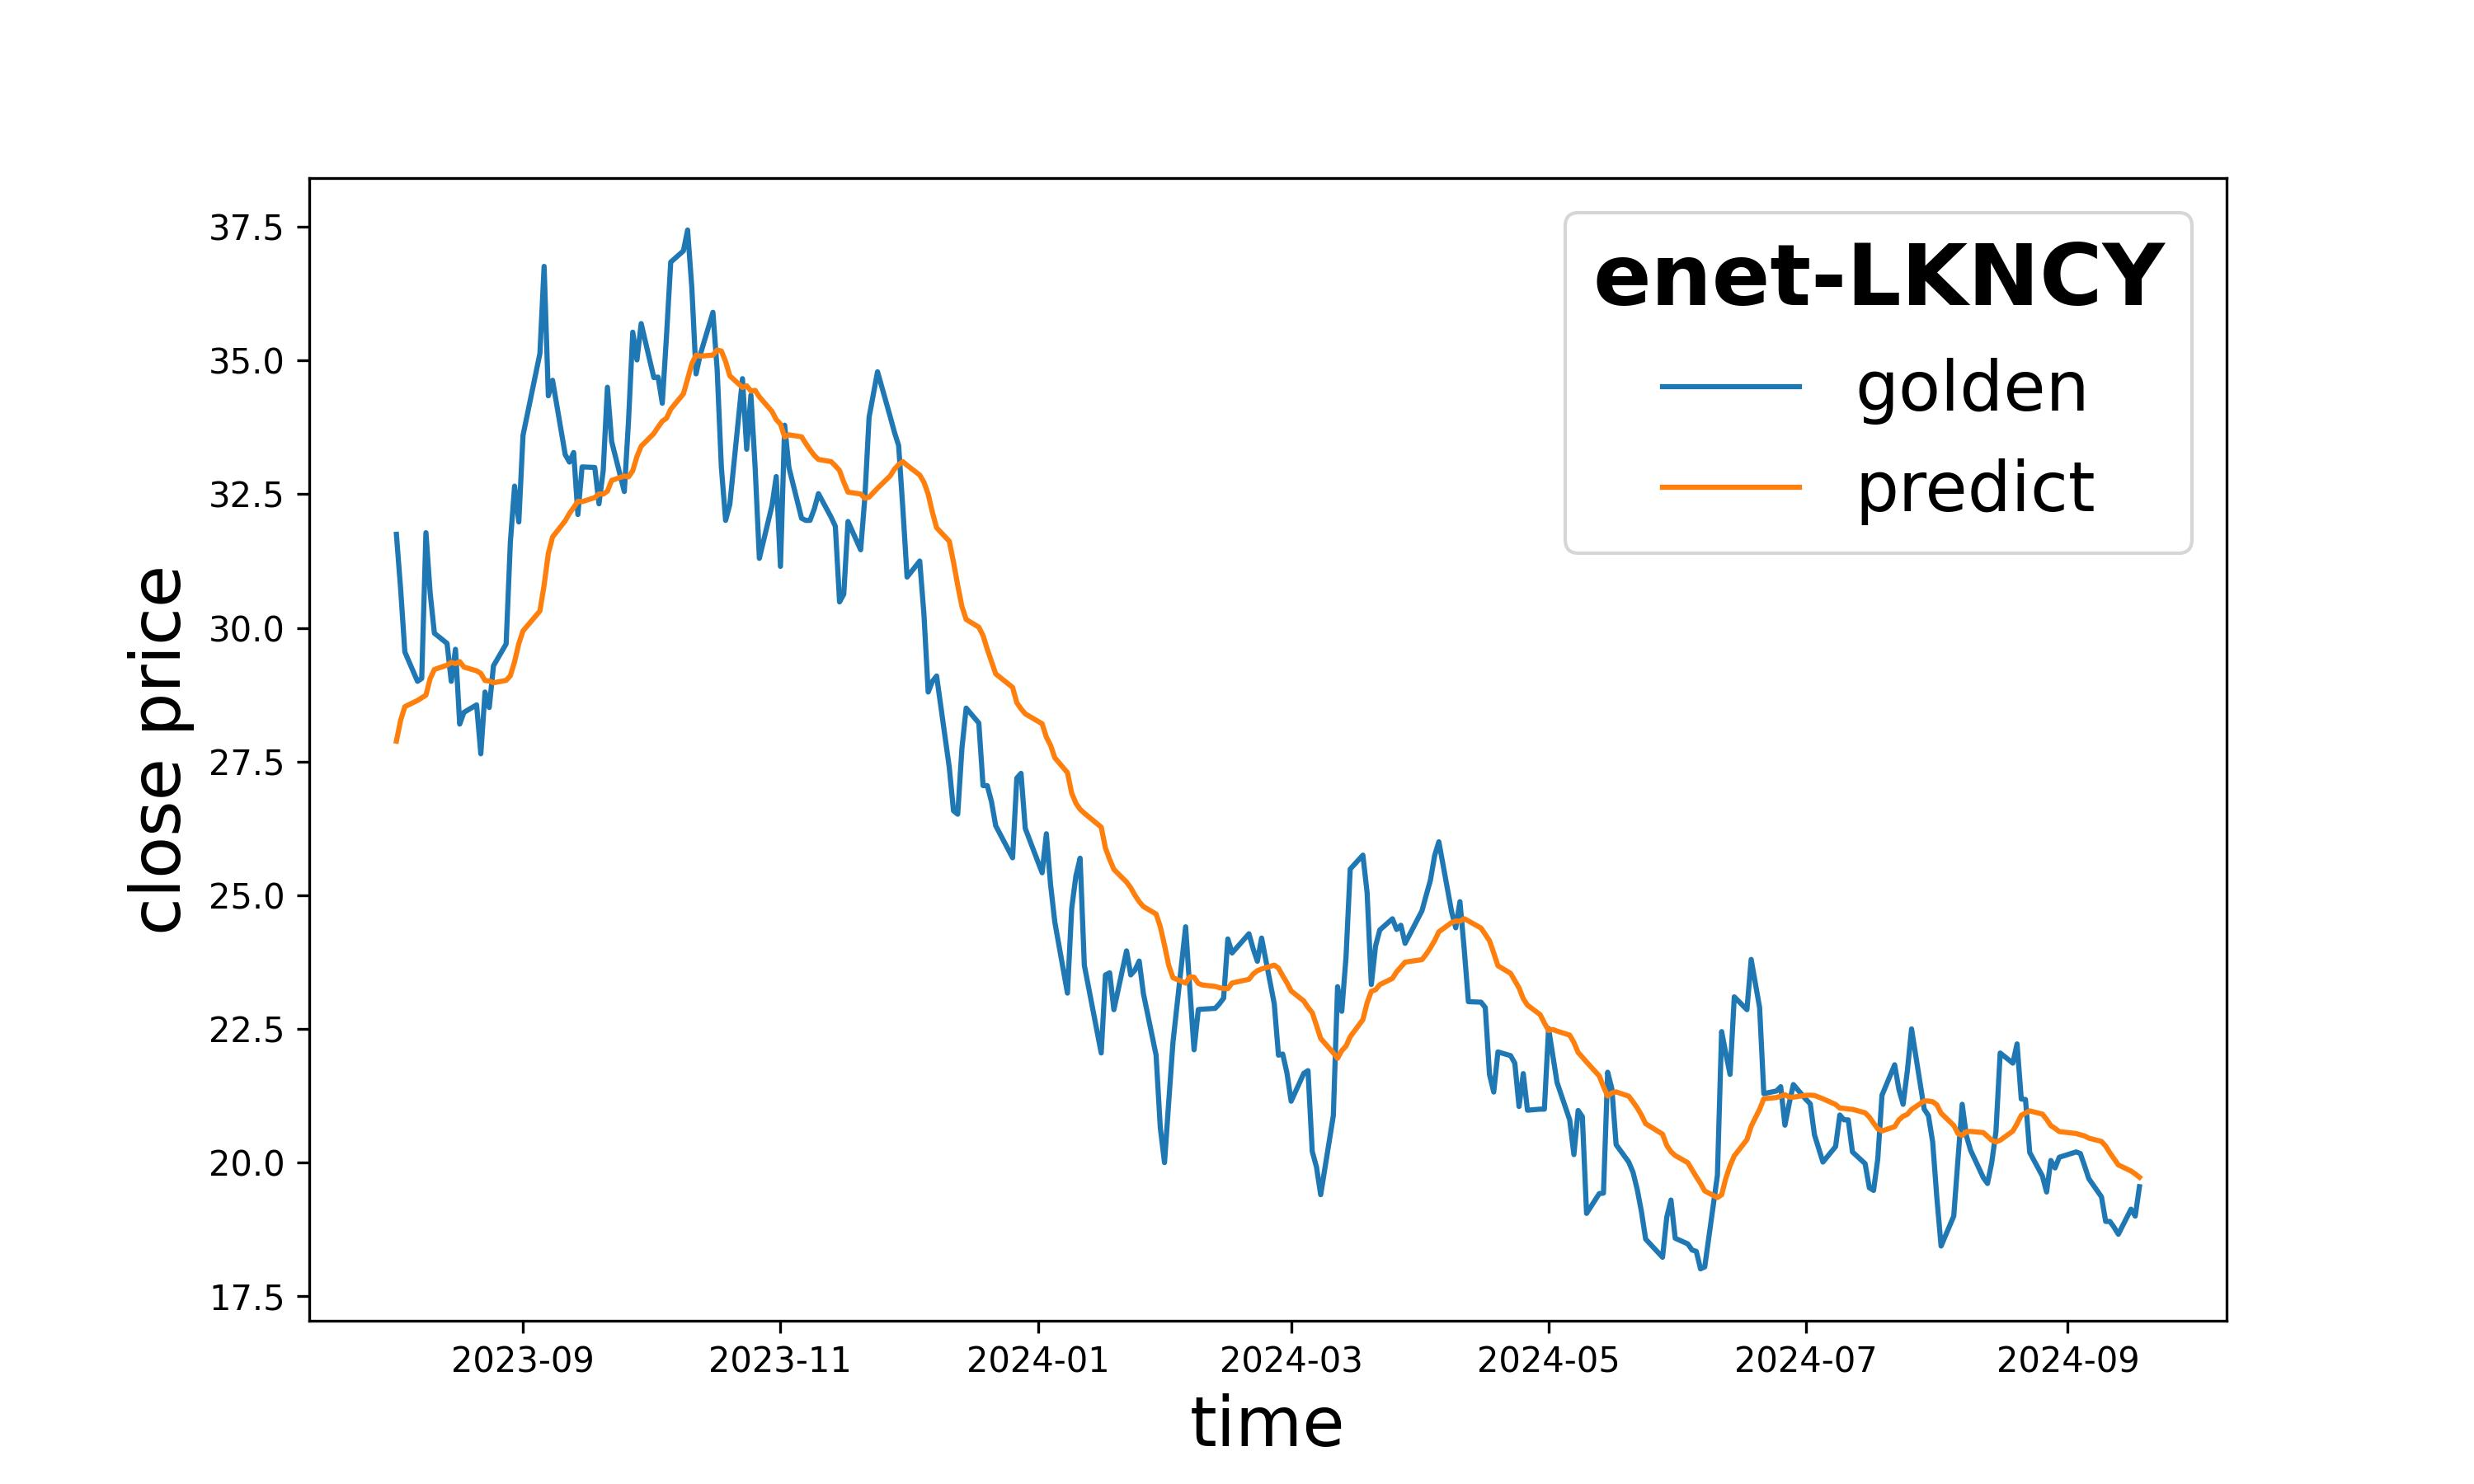
\includegraphics[width=\textwidth]{Result-Image/Result-Image3/07.LKNCY/enet-LKNCY.jpg}
        \caption{Enet}
        \label{fig:image1}
    \end{subfigure}
    \hfill
    \begin{subfigure}[b]{0.49\textwidth}
        \centering
        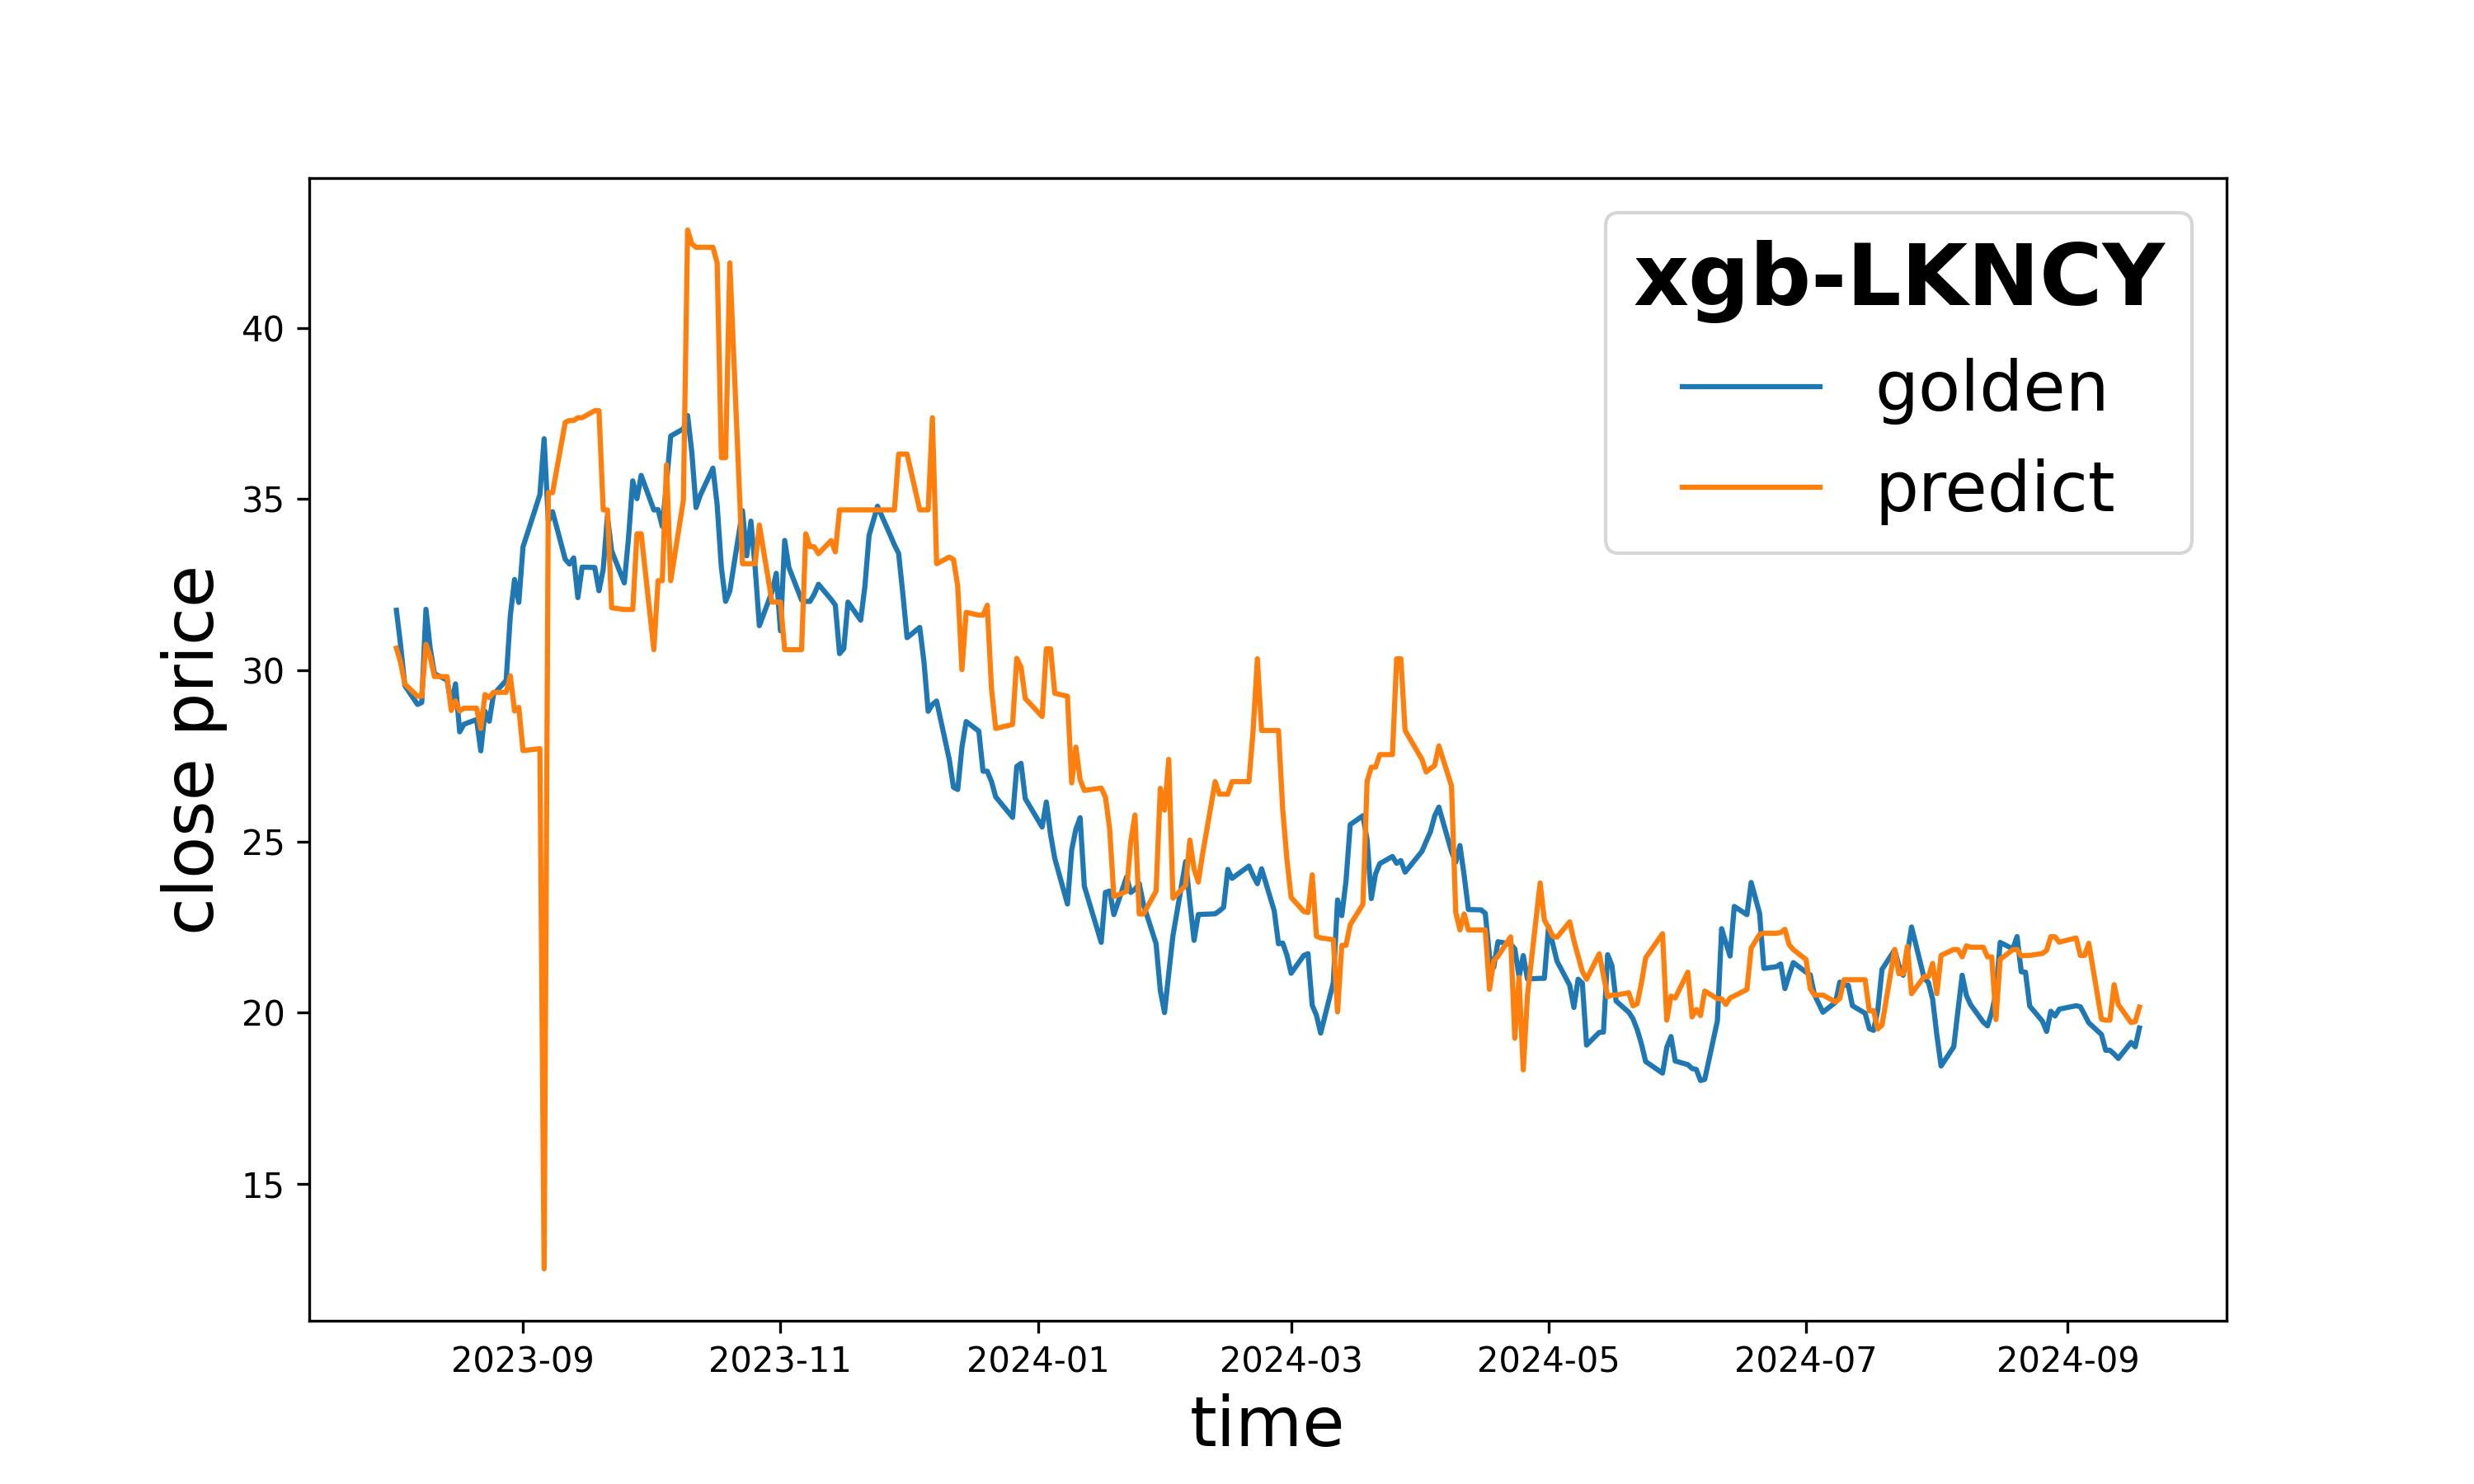
\includegraphics[width=\textwidth]{Result-Image/Result-Image3/07.LKNCY/xgb-LKNCY.jpg}
        \caption{XGBoost}
        \label{fig:image2}
    \end{subfigure}
    
    % 두 번째 행
    \vskip\baselineskip
    \begin{subfigure}[b]{0.49\textwidth}
        \centering
        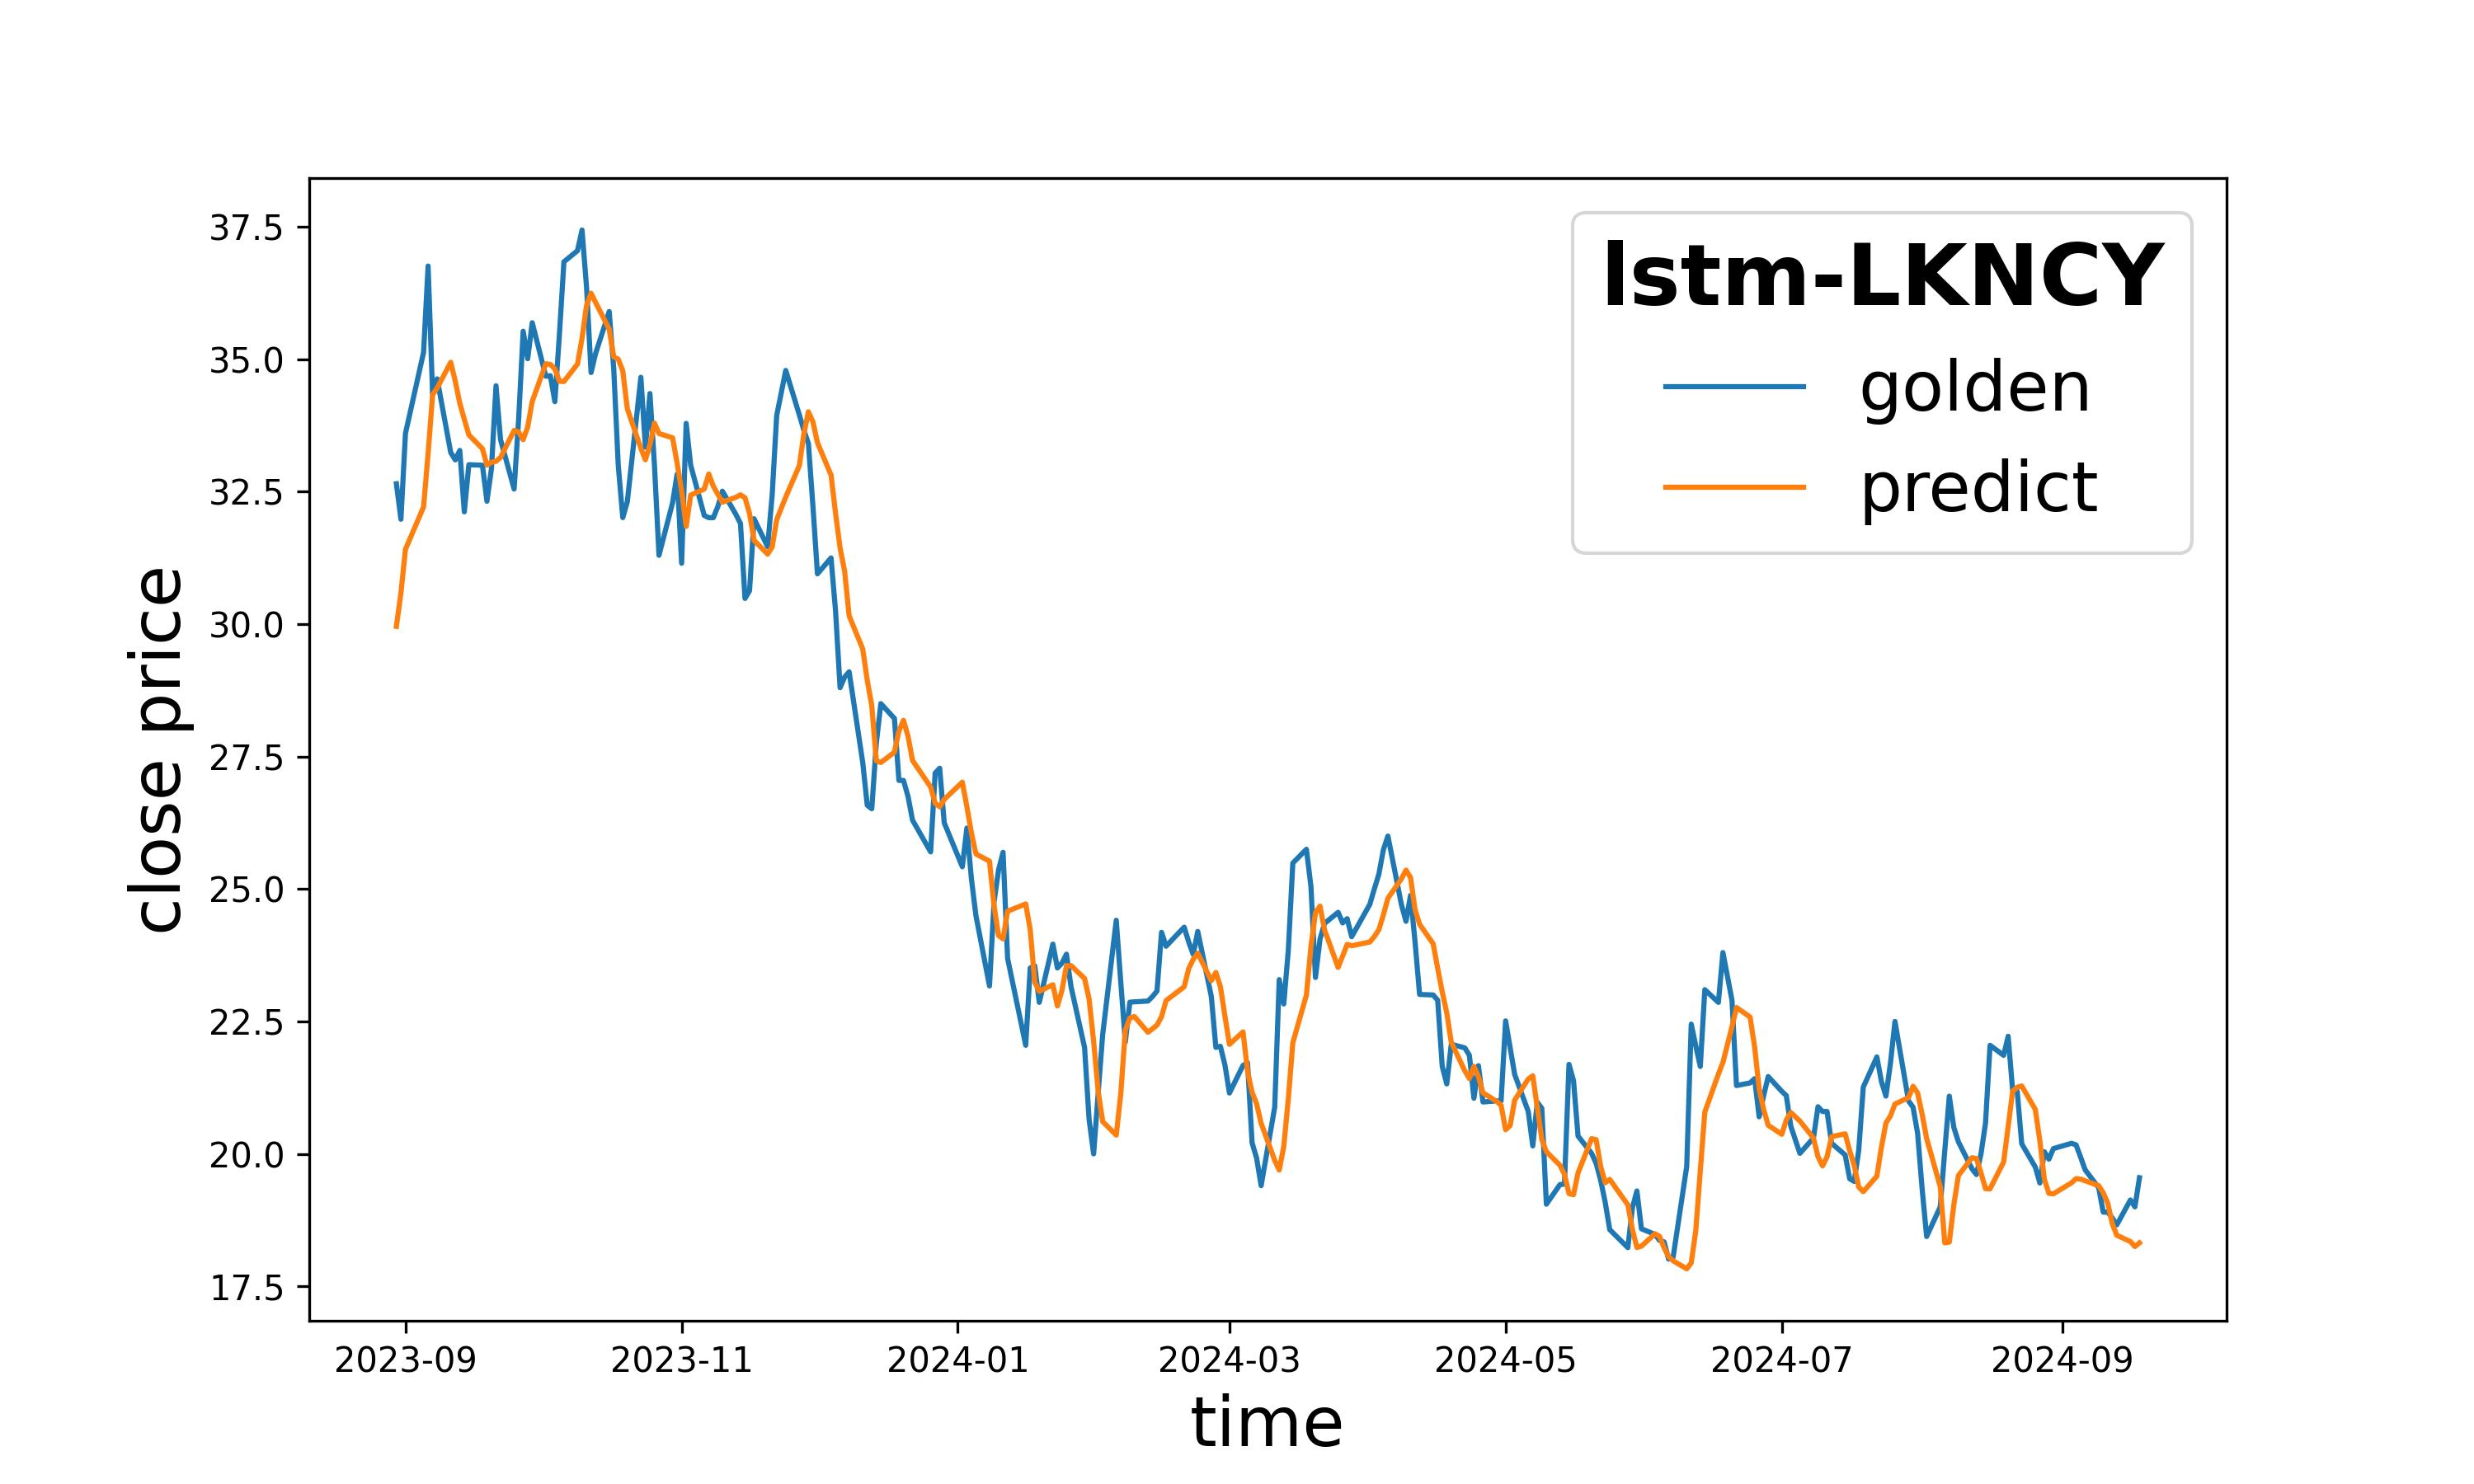
\includegraphics[width=\textwidth]{Result-Image/Result-Image3/07.LKNCY/lstm-LKNCY.jpg}
        \caption{LSTM}
        \label{fig:image3}
    \end{subfigure}
    \hfill
    \begin{subfigure}[b]{0.49\textwidth}
        \centering
        \includegraphics[width=\textwidth]{Result-Image/Result-Image3/07.LKNCY/arima_lstm-LKNCY.jpg}
        \caption{ARIMA-LSTM}
        \label{fig:image4}
    \end{subfigure}
    
    \caption{LKNCY}
    \label{fig:2x2grid}
\end{figure}



%\subsection{PZZA}
\begin{figure}[ht]
    \centering
    \begin{subfigure}[b]{0.49\textwidth}
        \centering
        \includegraphics[width=\textwidth]{Result-Image/Result-Image3/08.PZZA/PZZA.jpg}
        \caption{Training/Testing}
        \label{fig:image1}
    \end{subfigure}

    
    % 첫 번째 행
    \begin{subfigure}[b]{0.49\textwidth}
        \centering
        \includegraphics[width=\textwidth]{Result-Image/Result-Image3/08.PZZA/enet-PZZA.jpg}
        \caption{Enet}
        \label{fig:image1}
    \end{subfigure}
    \hfill
    \begin{subfigure}[b]{0.49\textwidth}
        \centering
        \includegraphics[width=\textwidth]{Result-Image/Result-Image3/08.PZZA/xgb-PZZA.jpg}
        \caption{XGBoost}
        \label{fig:image2}
    \end{subfigure}
    
    % 두 번째 행
    \vskip\baselineskip
    \begin{subfigure}[b]{0.49\textwidth}
        \centering
        \includegraphics[width=\textwidth]{Result-Image/Result-Image3/08.PZZA/lstm-PZZA.jpg}
        \caption{LSTM}
        \label{fig:image3}
    \end{subfigure}
    \hfill
    \begin{subfigure}[b]{0.49\textwidth}
        \centering
        \includegraphics[width=\textwidth]{Result-Image/Result-Image3/08.PZZA/arima_lstm-PZZA.jpg}
        \caption{ARIMA-LSTM}
        \label{fig:image4}
    \end{subfigure}
    
    \caption{PZZA}
    \label{fig:2x2grid}
\end{figure}

%\subsection{SBUX}
\begin{figure}[ht]
    \centering
    \begin{subfigure}[b]{0.49\textwidth}
        \centering
        \includegraphics[width=\textwidth]{Result-Image/Result-Image3/09.SBUX/SBUX.jpg}
        \caption{Training/Testing}
        \label{fig:image1}
    \end{subfigure}
    
    % 첫 번째 행
    \begin{subfigure}[b]{0.49\textwidth}
        \centering
        \includegraphics[width=\textwidth]{Result-Image/Result-Image3/09.SBUX/enet-SBUX.jpg}
        \caption{Enet}
        \label{fig:image1}
    \end{subfigure}
    \hfill
    \begin{subfigure}[b]{0.49\textwidth}
        \centering
        \includegraphics[width=\textwidth]{Result-Image/Result-Image3/09.SBUX/xgb-SBUX.jpg}
        \caption{XGBoost}
        \label{fig:image2}
    \end{subfigure}
    
    % 두 번째 행
    \vskip\baselineskip
    \begin{subfigure}[b]{0.49\textwidth}
        \centering
        \includegraphics[width=\textwidth]{Result-Image/Result-Image3/09.SBUX/lstm-SBUX.jpg}
        \caption{LSTM}
        \label{fig:image3}
    \end{subfigure}
    \hfill
    \begin{subfigure}[b]{0.49\textwidth}
        \centering
        \includegraphics[width=\textwidth]{Result-Image/Result-Image3/09.SBUX/arima_lstm-SBUX.jpg}
        \caption{ARIMA-LSTM}
        \label{fig:image4}
    \end{subfigure}
    
    \caption{SBUX}
    \label{fig:2x2grid}
\end{figure}


%\subsection{YUM}
\begin{figure}[ht]
    \centering
    \begin{subfigure}[b]{0.49\textwidth}
        \centering
        \includegraphics[width=\textwidth]{Result-Image/Result-Image3/10.YUM/YUM.jpg}
        \caption{Training/Testing}
        \label{fig:image1}
    \end{subfigure}
    
    % 첫 번째 행
    \begin{subfigure}[b]{0.49\textwidth}
        \centering
        \includegraphics[width=\textwidth]{Result-Image/Result-Image3/10.YUM/enet-YUM.jpg}
        \caption{Enet}
        \label{fig:image1}
    \end{subfigure}
    \hfill
    \begin{subfigure}[b]{0.49\textwidth}
        \centering
        \includegraphics[width=\textwidth]{Result-Image/Result-Image3/10.YUM/xgb-YUM.jpg}
        \caption{XGBoost}
        \label{fig:image2}
    \end{subfigure}
    
    % 두 번째 행
    \vskip\baselineskip
    \begin{subfigure}[b]{0.49\textwidth}
        \centering
        \includegraphics[width=\textwidth]{Result-Image/Result-Image3/10.YUM/lstm-YUM.jpg}
        \caption{LSTM}
        \label{fig:image3}
    \end{subfigure}
    \hfill
    \begin{subfigure}[b]{0.49\textwidth}
        \centering
        \includegraphics[width=\textwidth]{Result-Image/Result-Image3/10.YUM/arima_lstm-YUM.jpg}
        \caption{ARIMA-LSTM}
        \label{fig:image4}
    \end{subfigure}
    
    \caption{YUM}
    \label{fig:2x2grid}
\end{figure}



{\color{blue}In this section, you will list some experimental results with
some comparisons with some baseline methods.

For example, you choose to use SVM on a new dataset. Possible
baselines would be linear perceptron and logistic regression by
%using the same set of features.

In the final version, this part should
be about 2.5 page.}

\section{Conclusion}


This study showed that the LSTM model outperformed other models, including Enet, XGBoost, and LSTM-ARIMA, with the lowest MSE, RMSE, and MAE, and the highest $R^2$ value. This highlights LSTM as highly suitable for predicting complex time series data like stock market prices. The Enet model was effective in learning simple linear relationships but failed to adequately capture the characteristics of time series data. XGBoost, while a strong model for learning nonlinear patterns, lacked sufficient optimization. ARIMA-LSTM, as a combined time series model, underperformed compared to expectations, indicating a need for further optimization and improvement.\\

In conclusion, this study reaffirms the superiority of the LSTM model in stock market price prediction.  Future research could focus on enhancing the performance of the LSTM model through methods such as data augmentation, hyperparameter tuning, and incorporating additional external variables. Additionally, exploring ways to improve the performance of hybrid models like ARIMA-LSTM offers a promising avenue for further study.



{\color{blue}In this section, briefly discuss your conclusion for this project.
You can also talk about the future plan.

This part should be about 0.5 page.}


\begin{thebibliography}{99}  % '99' is the width of the citation label

\bibitem{Kontopoulou}
Kontopoulou, Vaia I. and Panagopoulos, Athanasios D. and Kakkos, Ioannis and Matsopoulos, George K.,
 \textit{A Review of ARIMA vs. Machine Learning Approaches for Time Series Forecasting in Data Driven Networks},
 MDPI, vol. 15(8), pages 1-31, July.
 
\bibitem{rabbit}
Burak Gülmez,
\textit{Stock price prediction with optimized deep LSTM network with artificial rabbits optimization algorithm},
Expert Systems With Applications 227 (2023) 120346.

\bibitem{hybrid}
R. Zhu, Y. Yang and J. Chen, 
\textit{XGBoost and CNN-LSTM hybrid model with Attention-based stock prediction},
 2023 IEEE 3rd International Conference on Electronic Technology, Communication and Information (ICETCI), Changchun, China, 2023, pp. 359-365.

\bibitem{lstm}
C. Jin, Z. Shi, W. Li, and Y.,
\textit{Bidirectional lstm-crf attention-based model for chinese word segmentation}. arXiv preprint arXiv:2105.09681, 2021.



\end{thebibliography}


\end{document}
